%%\documentclass[%
%% aip,
%% jmp,%
%% amsmath,amssymb,nofootinbib,
%%preprint,%
%%%reprint,%
%%%author-year,%
%%%author-numerical,%
%%]{revtex4-1}

\documentclass[preprint,5p]{elsarticle}

\usepackage{graphicx}% Include figure files
\usepackage{dcolumn}% Align table columns on decimal point
\usepackage{bm}% bold math
\usepackage{pennames}
\usepackage{subfigure}
\usepackage{amsmath}
\usepackage{float,verbatim,hyperref}
\usepackage[mathlines]{lineno}% Enable numbering of text and display math
\modulolinenumbers[5]% https://www.overleaf.com/5788191175jnrbsnhpffds[5]
\linenumbers\relax % Commence numbering lines

\begin{document}

\date{\today}% It is always \today, today,
             %  but any date may be explicitly specified

\begin{frontmatter}
\title{X-ray Scanning Technique For Alignment of Photodetectors}
\author[uci]{William Kyle}
\author[uci]{Terence Libeiro}
\address[uci]{University of California, Irvine}

\begin{abstract}
The X-ray survey technique is designed to systematically survey the position
of photodetectors installed as part of the calorimeter upgrade of the MEG experiment.
The photosensitive surface is scanned in axial (Z) and azimuthal ($\phi$) directions
with a precisely controlled, thin collimated beam of X-ray obtained from \cob X-ray source.
Systematic shifts as well as small deformations are observed 
which result from the assembly of photodetectors and the cryogenic cooling of
of the liquid Xenon scintillator. Analysis of data shows in-situ positions of the photodetectors
deviate from the expectation by 2~mm in Z coordinate and a maximum 5~mm in $\phi$
coordinate. An uncertainty of 0.3~mm is attributed to the calculated positions
well within the resolution goals for photon reconstruction in second run of the MEG experiment.

\end{abstract}
\end{frontmatter}
%\tableofcontents



%\maketitle

\section{\label{intro}Introduction}
The MEG experiment is designed to search for charged flavor violating
\mueg process (cLFV) in muon decays \cite{megexperiment}.  While
exceedingly small branching ratio ($B < 10^{-50}$) postulated by the
Standard Model (SM) prevents the charged flavor exchange process to be
observed directly, it provides a clean background free mode of
searching for beyond the Standard Model physics.  Extensions to the
Standard Model with Supersymmetry (SUSY) have been posited to explain
the apparent lightness of neutrino masses and flavor violation via
oscillations, as well as for the broader goal of unifying all the SM
gauge groups. Searches for new physics with cLFV processes are
underway motivated by the fact that the rates of such processes
enhanced by SUSY are just within the design sensitivities of the
current experiments.  Results from the LHC so far have ruled out the
existence of supersymmetric particles in the mass range 1-2 TeV
\cite{lhcsusy1,lhcsusy2}, and failed to observe charged flavor violating
process\cite{lhcclfv1,lhcclfv2}.  Given the upper limit of
direct detection at the LHC, indirect searches such as MEG provide a
powerful and complimentary probe of investigating cLFV.  To-date no
evidence has been observed, the world’s most sensitive limit was set
by the MEG experiment $B < 4.2 \times 10^{-14}$ at 90\% CL using data
collected in the running period 2009-2013 (Run~I) \cite{meg1result}.
An upgraded detector components and beam conditions in the MEG
experiment aim to improve this measurement by an order of magnitude in
the second run (2019-2022).  The entrance face of the liquid Xe (LXe)
calorimeter of MEG was upgraded with MPPC (Multi-Pixel Photon counter)
photodetectors to provide improved photon detection and
reconstruction.  This paper describes the X-ray survey conducted to
determine absolute in-situ positions of these photodetectors.

\section{\label{motivation}Motivation}
Relative alignment of the photodetectors and the positron
spectrometer is essential in MEG to realize the acceptance
requirements of \mueg topology.  Although an alignment
using external markers on the LXe calorimeter is performed the
relative positions of the markers and the photodetectors is
subject to change. The photodetectors are enclosed in a
cryostat and the volume of the inner 
calorimeter is filled with liquid Xenon and cooled to 170~K. 
The in-situ position of the
detectors is affected by thermal contraction and buoyant
forces which cannot be easily modeled or predicted. In the
previous MEG run a linear deformation model was used to
correct for these effects which is no longer applicable due
to stringent resolution goals\cite{megdesign,megproposal}
(u$_\gamma$/v$_\gamma$ 5/5~mm (Run I) vs 2.6/2.2 mm (Run II))
of this run for photon reconstruction.  An increased photosensitive
area in the upgraded calorimeter requires a systematic survey
that can scan with higher precision than possible with the
studies using charge exchange reaction \cex in an stationary
liquid hydrogen target, conducted in Run~I.  An X-ray survey of
the detector is conceived to determine the absolute position
of the photodetectors inside the LXe calorimeter. The design,
operation and data analysis with the X-ray technique is
documented in the following sections.




\section{Calorimeter}\label{sec:calorimeter}

The LXe calorimeter is a homogenous calorimeter using liquid Xenon scintillator
enclosed in a semi-cylindrical (C-shaped) volume placed around the COBRA magent
\cite{megdesign}.  It is designed to detect prompt scintialltion light from
photons originating in \muon decays, interacting at LXe temperature 170~K in the
VUV range ($\lambda = 175 \pm 5$ nm).  The surface of the enclosed volume is
covered with two different photodetectors, the inner face  with MPPC and the
rest of the surfaces with 2-inch PMT.  The axis of the cylindrical calorimeter
is nominally aligned with the Z axis in MEG coordinate system.

The inner face of the LXe calorimeter consists of 4092 MPPCs arranged in a grid
structure containing 93 rows in the $\phi$ direction.  A row consists of 44
MPPCs placed along $\hat{z}$ direction, divided equally in two PCB\footnote{Printed
Circuit Board} strips, placed on the upstream ($Z<0$ mm) and downstream ($Z>0$
mm) sides of the calorimeter.  The PCB strips are mounted with spacer materials
on four CFRP\footnote{Carbon Fiber Reinforced Polymer} plates, each containing
23-24 strips and attached to the inner face of the cryostat at different $\phi$
locations.  
\begin{figure}
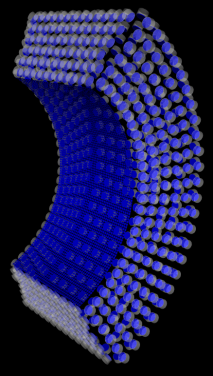
\includegraphics[height=4cm]{plots/LXeMEGUpgrade.png}
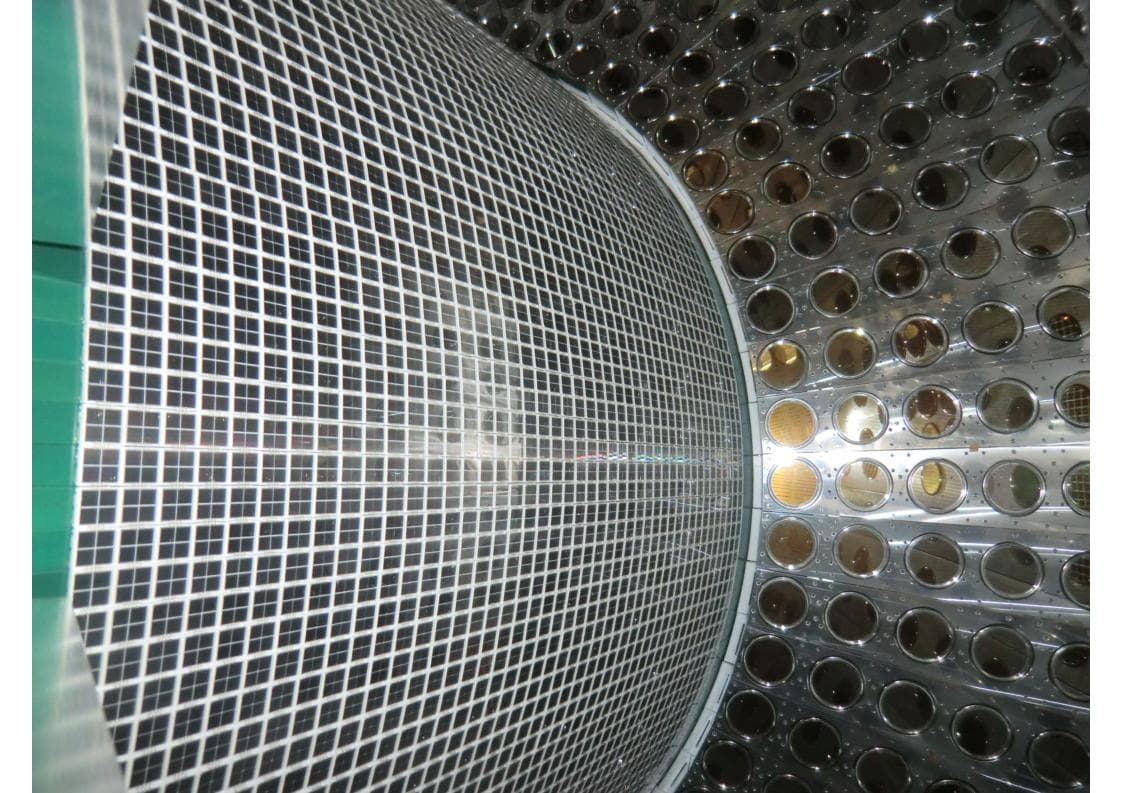
\includegraphics[height=4cm]{plots/CIMG5301}
\label{fig:calorimeter}
\caption{Liquid Xe calorimeter in the MEG experiment.}
\end{figure}
The MPPC photodetectors are developed according to the experimental
requirements with large photosensitive area 12 $\times$ 12 mm$^2$,
comprised of four  smaller pixels 6 $\times$ 6 mm$^2$ connected in
series.  The photodetectors are placed in a ceramic case (15 mm) and
mounted on a PCB strip, each containing 22 photodetectors.  Two
identically produced strips aligned along $\hat{z}$ direction, and
rotated by 180\degree with respect to each other to allow for
electronics readout at each end, make up a single row (fig 
\ref{fig:mppc}).
\begin{figure}
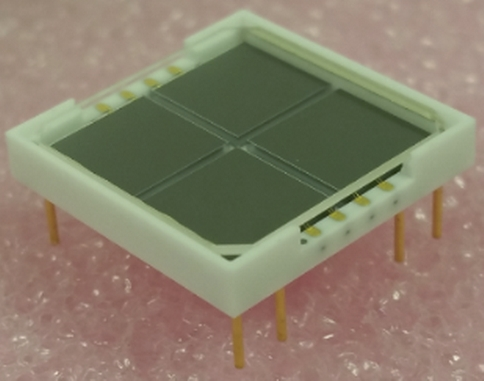
\includegraphics[width=3cm]{plots/single_mppc.jpg}
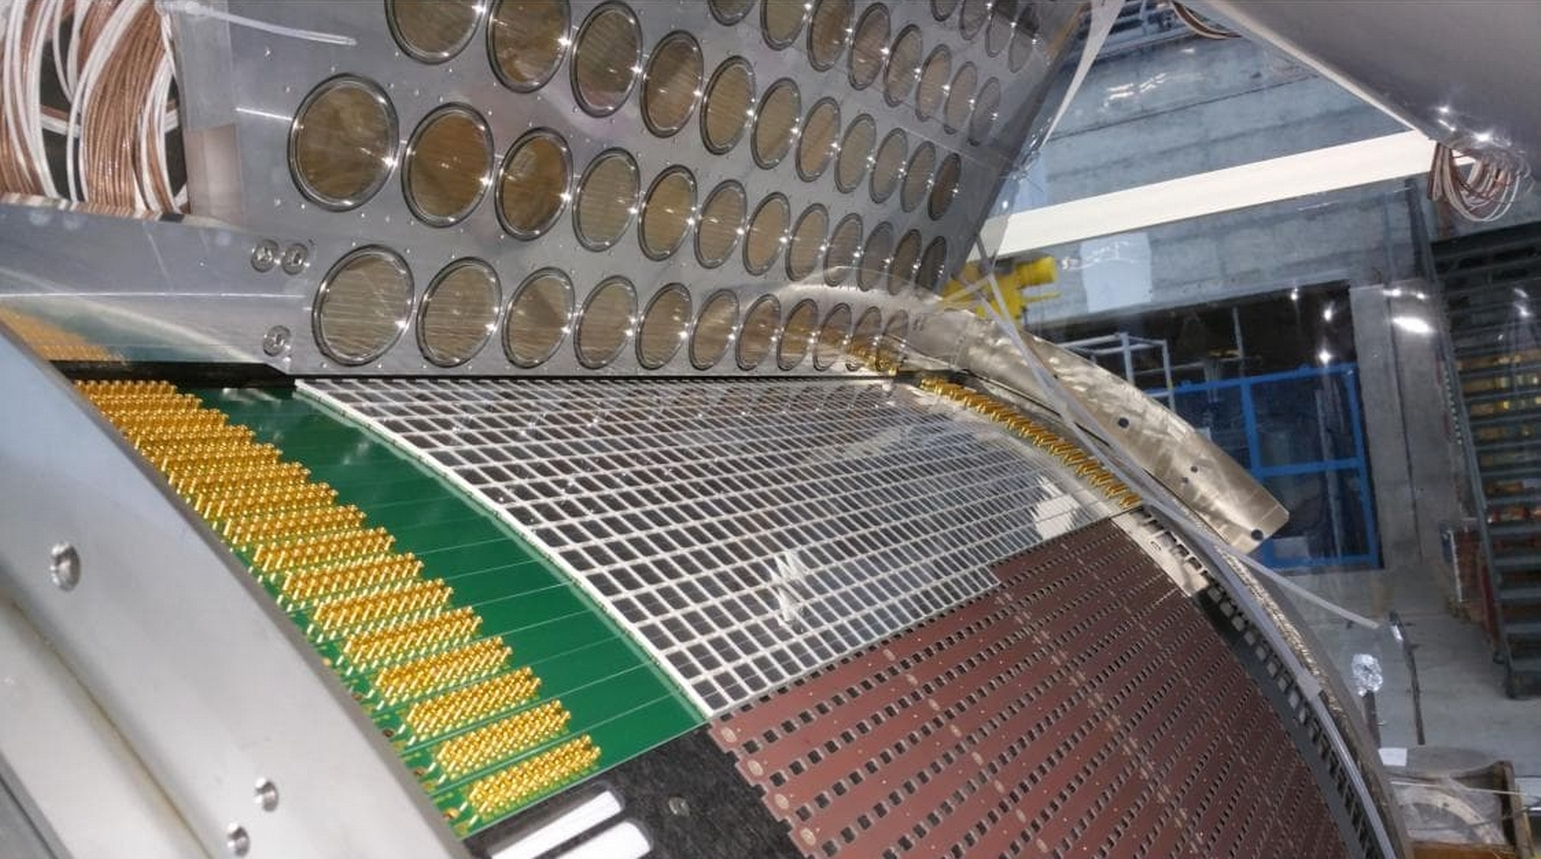
\includegraphics[width=5cm]{plots/CFRP_spacer_MPPC.jpg}
\caption{Single MPPC and installed MPPCs in the LXe calorimeter.}
\label{fig:mppc} 
\end{figure}



\section{\label{sec4}Alignment of apparatus}
\subsection{Optical alignment}

An optical survey was performed for securing a good alignment of the
X-ray survey apparatus with respect to the calorimeter.  Following
this procedure X-ray coordintes from the motion controllers 
can be simply translated in to standard MEG coordinates.
The motion stages allow the X-ray to be moved in axial (Z) and
azimuthal ($\phi$) directions.  Using  an optical survey the axial
motion of the collimator is aligned to coincide with the MEG Z~axis.
Additionally, the rotational plane of the collimator is also aligned
to the vertical plane.  This procedure is performed by measuring the
exact coordinates (x,y,z) and the rotation plane vectors (rx,ry,rz) of
the X-ray at multiple reference axial locations.  Minor
deviatons from the expected positions are recorded and subsequently
used in the correction procedure (next section).  The precision of the
alignment X-ray postion at the calorimeter is calculated to be 0.1~mm
(0.15~mrad) in Z ($\phi$).

\subsection{Degrees of freedom of the X-ray beam}
\label{sec:corrections}
    Small displacements in the linear stage during its motion
    introduces rotations in the X-ray beam. The changes in
    the X-ray position are monitored using a laser attached to the
    linear stage projected at a quadrant photodiode, and a bubble
    level. The laser system detects difference in intensity of the
    laser in horizontal and vertical directions which are translated
    into angular deviations about X and Y axes. Figure \ref{fig:dxdy}
    shows axial position dependent relative intensities in horizontal
    ($\frac{\mathrm{left-right}}{\mathrm{total}}$, blue) and vertical
    ($\frac{\mathrm{down-up}}{\mathrm{total}}$, red) directions and the
    corresponding angular deviations $<\pm$0.8~mrad.
    \begin{figure}[]
      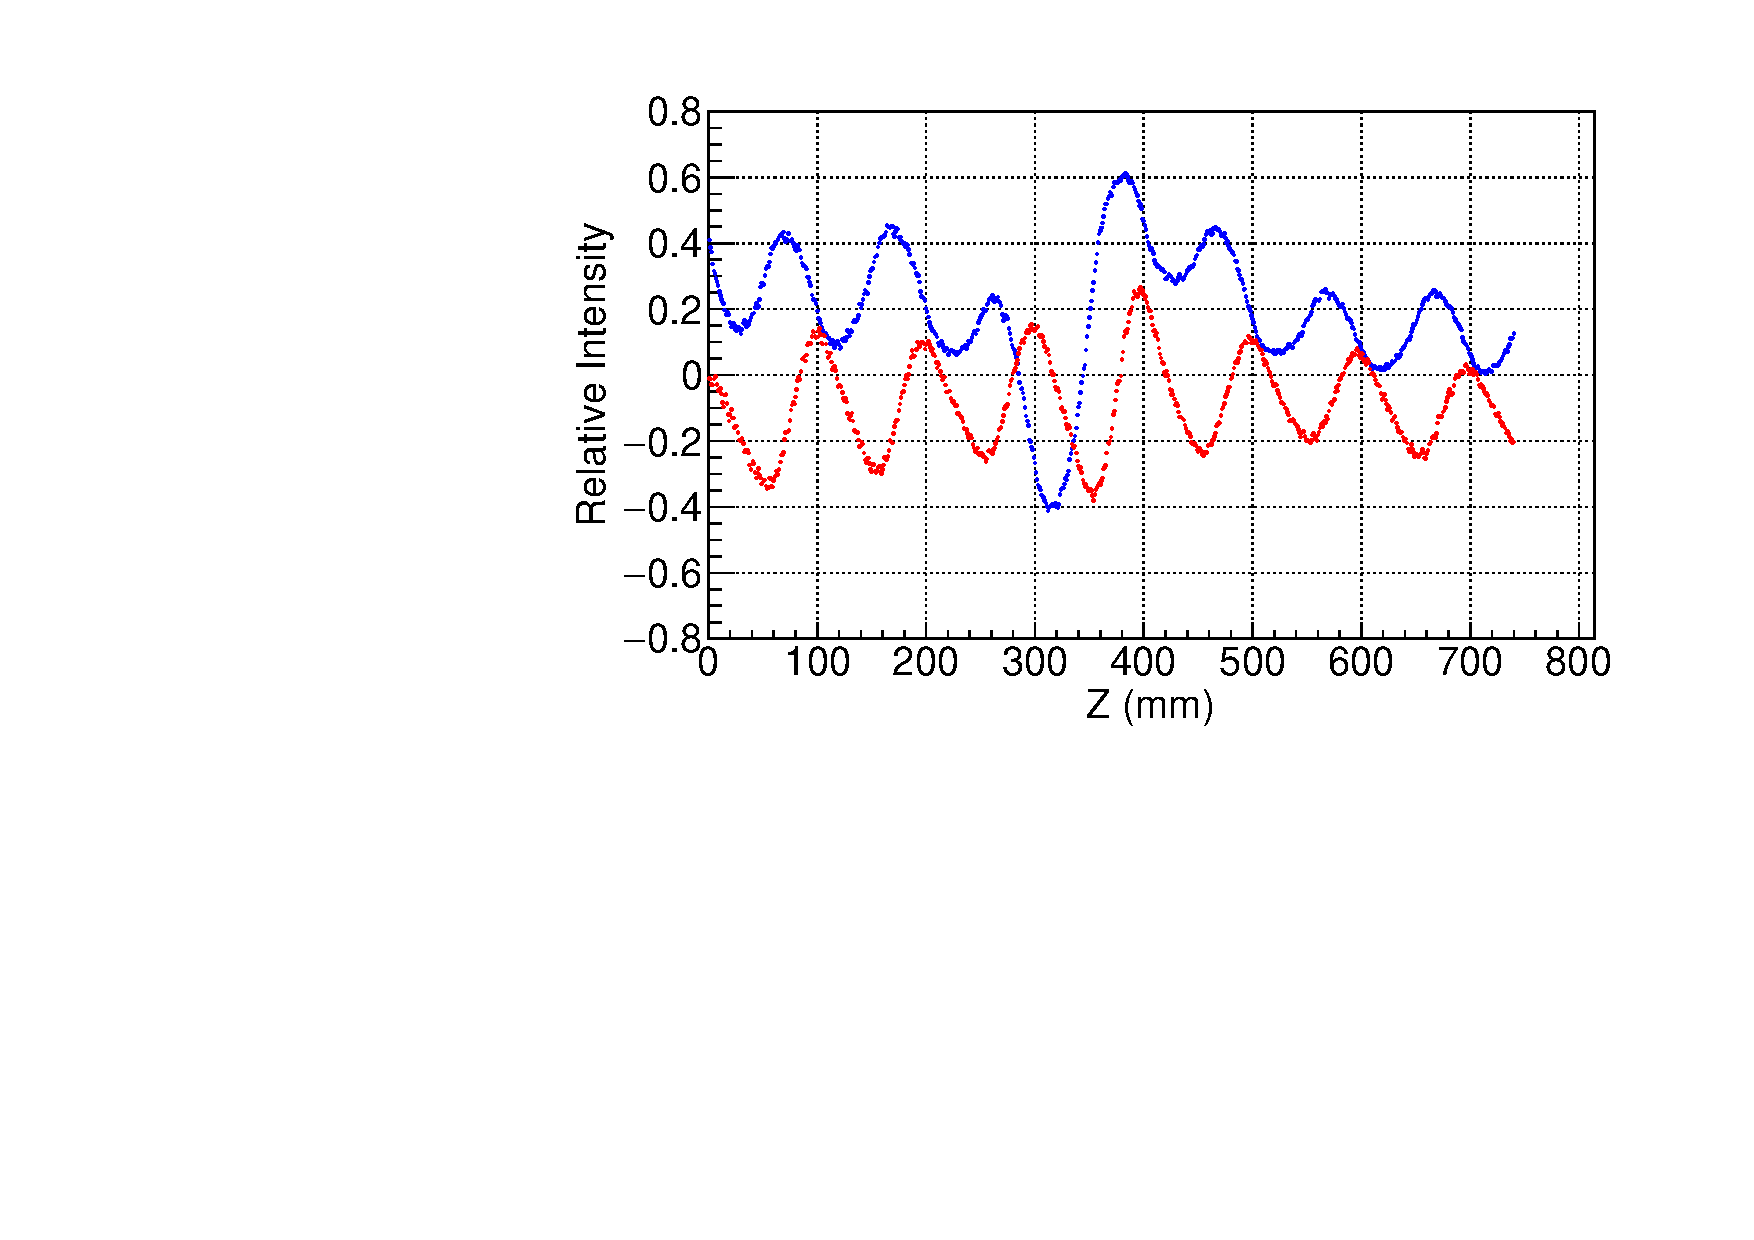
\includegraphics[width=4cm]{plots/rel_intensity}
      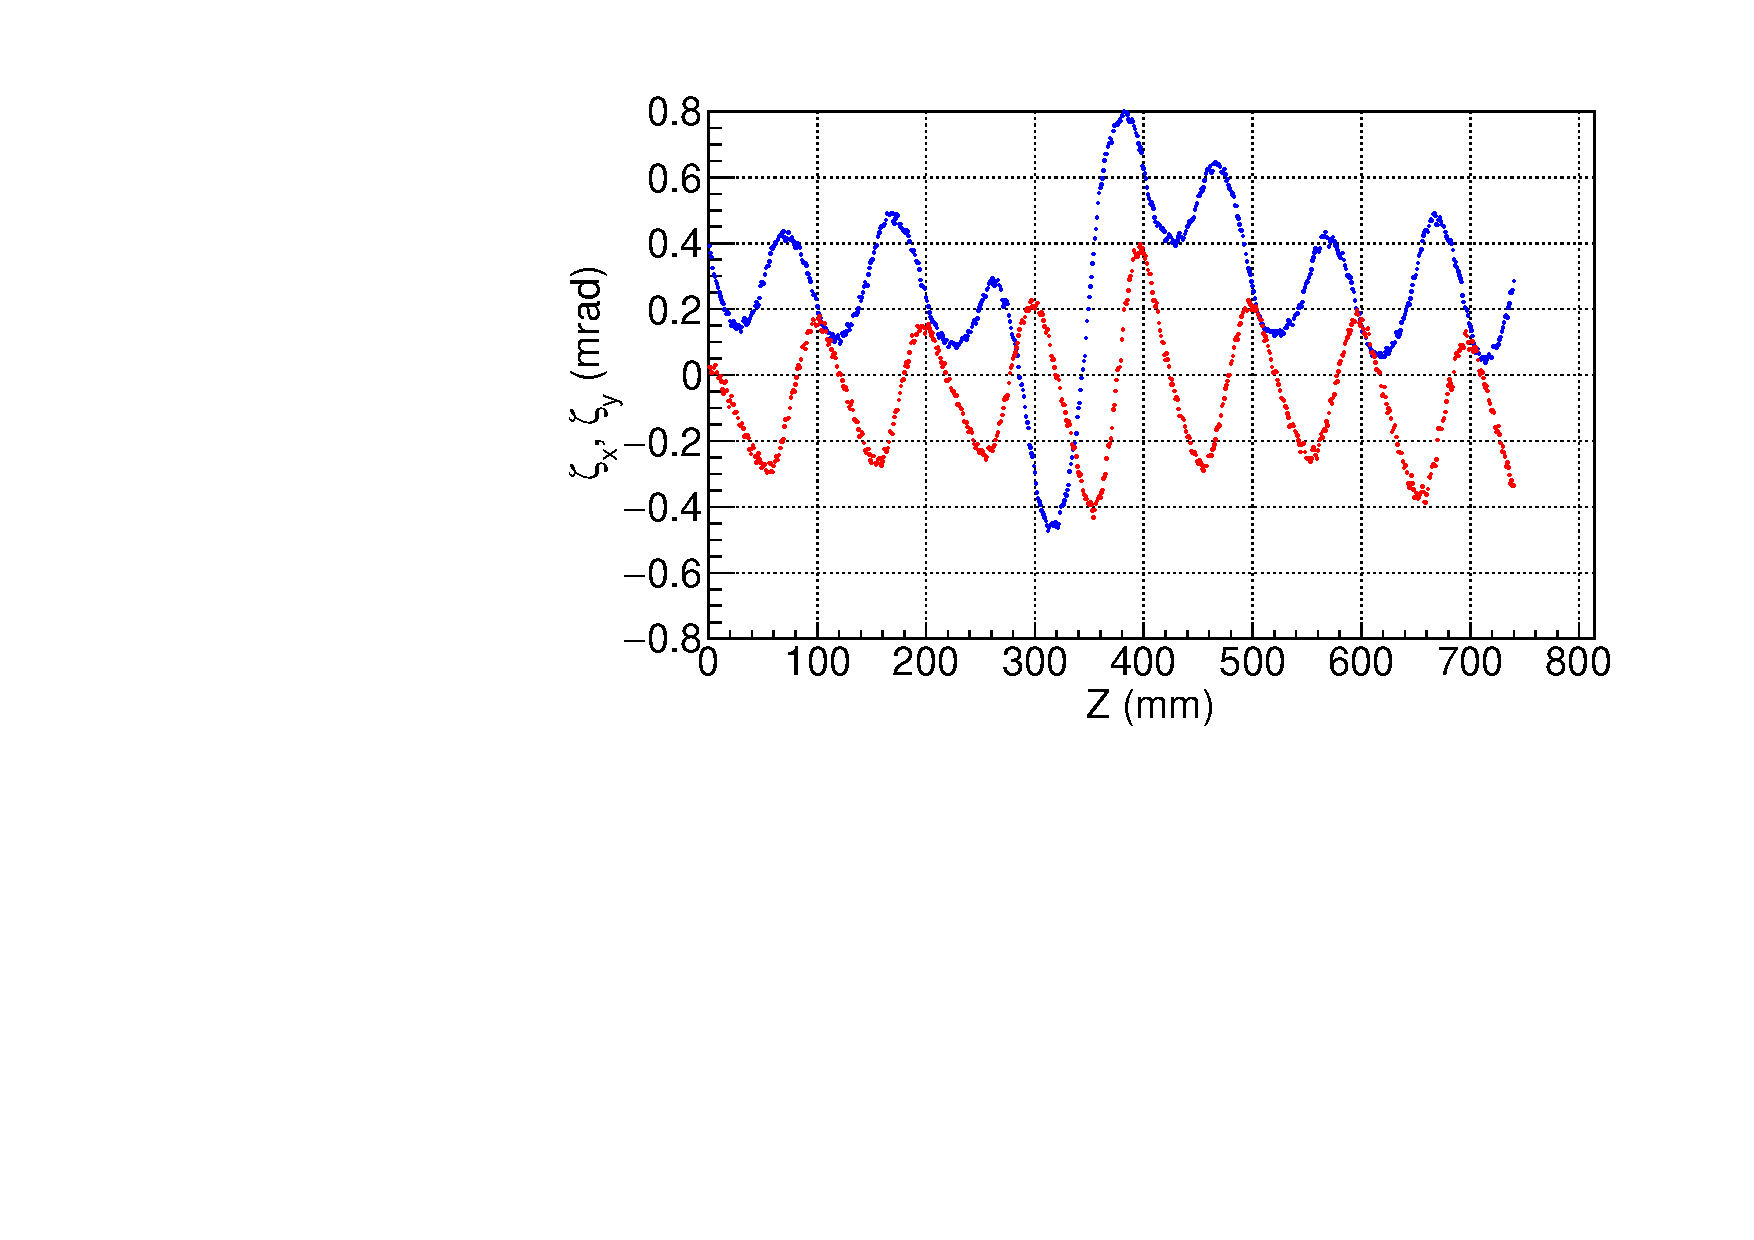
\includegraphics[width=4cm]{plots/angle_dx_dy}
      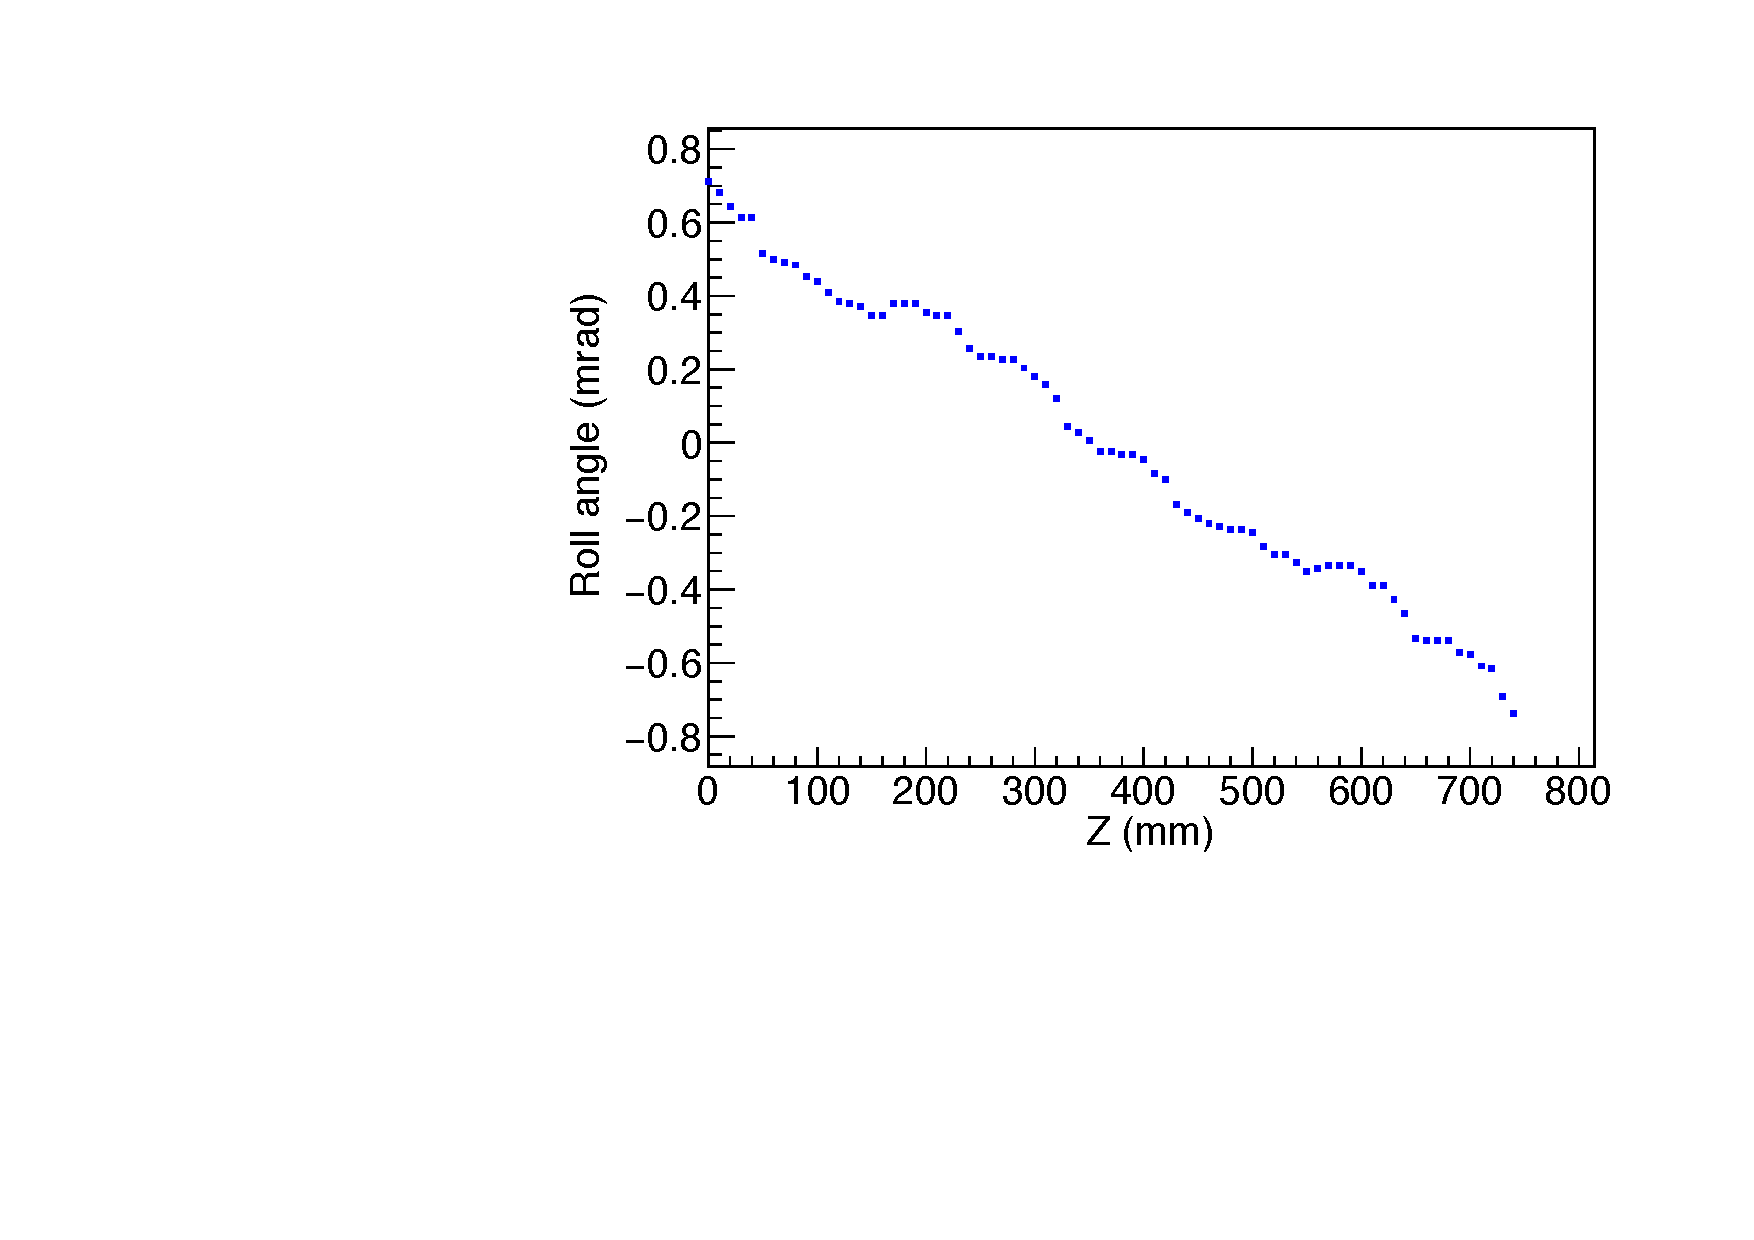
\includegraphics[width=4cm]{plots/BubbleLevel_June042017}
      \caption{Relative intensities in horizontal and vertical planes
      recorded by the laser monitoring system (left) and the calculated angular
      rotation (right).}

      \label{fig:dxdy}
    \end{figure}  
    The X-ray is projected in an orthogonal direction to the axis of the
    magnet. Working in the MEG coordinate system, the rotations of the
    X-ray about X and Y axes lead to a displacement in the Z coordinate of
    the X-ray at the calorimeter. For given angular rotations,
    $\zeta_x,\zeta_y$ about X and Y axes respectively, the correction in Z
    ($\Delta$Z) is proportional to the distance to the calorimeter (R) and
    the azimuthal angle ($\phi$) calculated as following

    \begin{align}
      \Delta Z(Z,\phi)_x &= -\zeta_x(Z)\,R\,cos(\phi)     \\
      \Delta Z(Z,\phi)_y &= \quad \zeta_y(Z)\,R\,sin(\phi) \\
      \Delta Z(Z,\phi)\  &= \quad \Delta Z_x + \Delta Z_y
    \end{align}

  A bubble level is used to detect the rotation of the X-ray
  collimator about Z~axis.  The position of the bubble is recorded
  with a 2~MP camera connected to Raspberry Pi device over the entire
  range of the linear stage.  A photograph is taken every 10~mm and
  the position of the bubble is interpolated at all intermediate
  locations. The photographs provide raw data which is converted into
  relative position of the bubble using pixel tracking
  software\cite{imagej} and calibrated to absolute rotation angle
  using the optical survey data(Figure~\ref{fig:bubblelevel}).  A
  correction is equal to the rotation angle about Z~axis, is added to
  the nominal $\phi$ value. Nominally, the X-ray collimator is fixed
  to the rotation stage    such that the centers of collimator and the
  rotational motion     coincide. However, optical surveys performed
  in the running period     show slight misalignment between the two
  in the vertical plane     ($\sim$100$\micron$).  This induces a
  $\phi$ dependent shift in the     $\phi$ coordinate of the X-ray;
  the effect on the Z coordinate is     found to be negligible. The
  correction to $\phi$ coordinates are calculated analtically
  considering the change in nominal and     displaced X-ray vectors at
  the calorimeter. Given the angular     rotation $\zeta_z$ about
  Z-axis, and the angular offset $d\phi_{coll}$     due to displaced
  collimator center, the $\phi$ correction      ($\Delta\phi$) is
  calculated as 

  \begin{align} 
  \Delta \phi (Z,\phi) = \zeta_z(Z)+d\phi_{coll}(Z,\phi) 
  \end{align}

  %%Z axis in plots must be converted to MEG coordinates, axis labels.
    \begin{figure}[]
        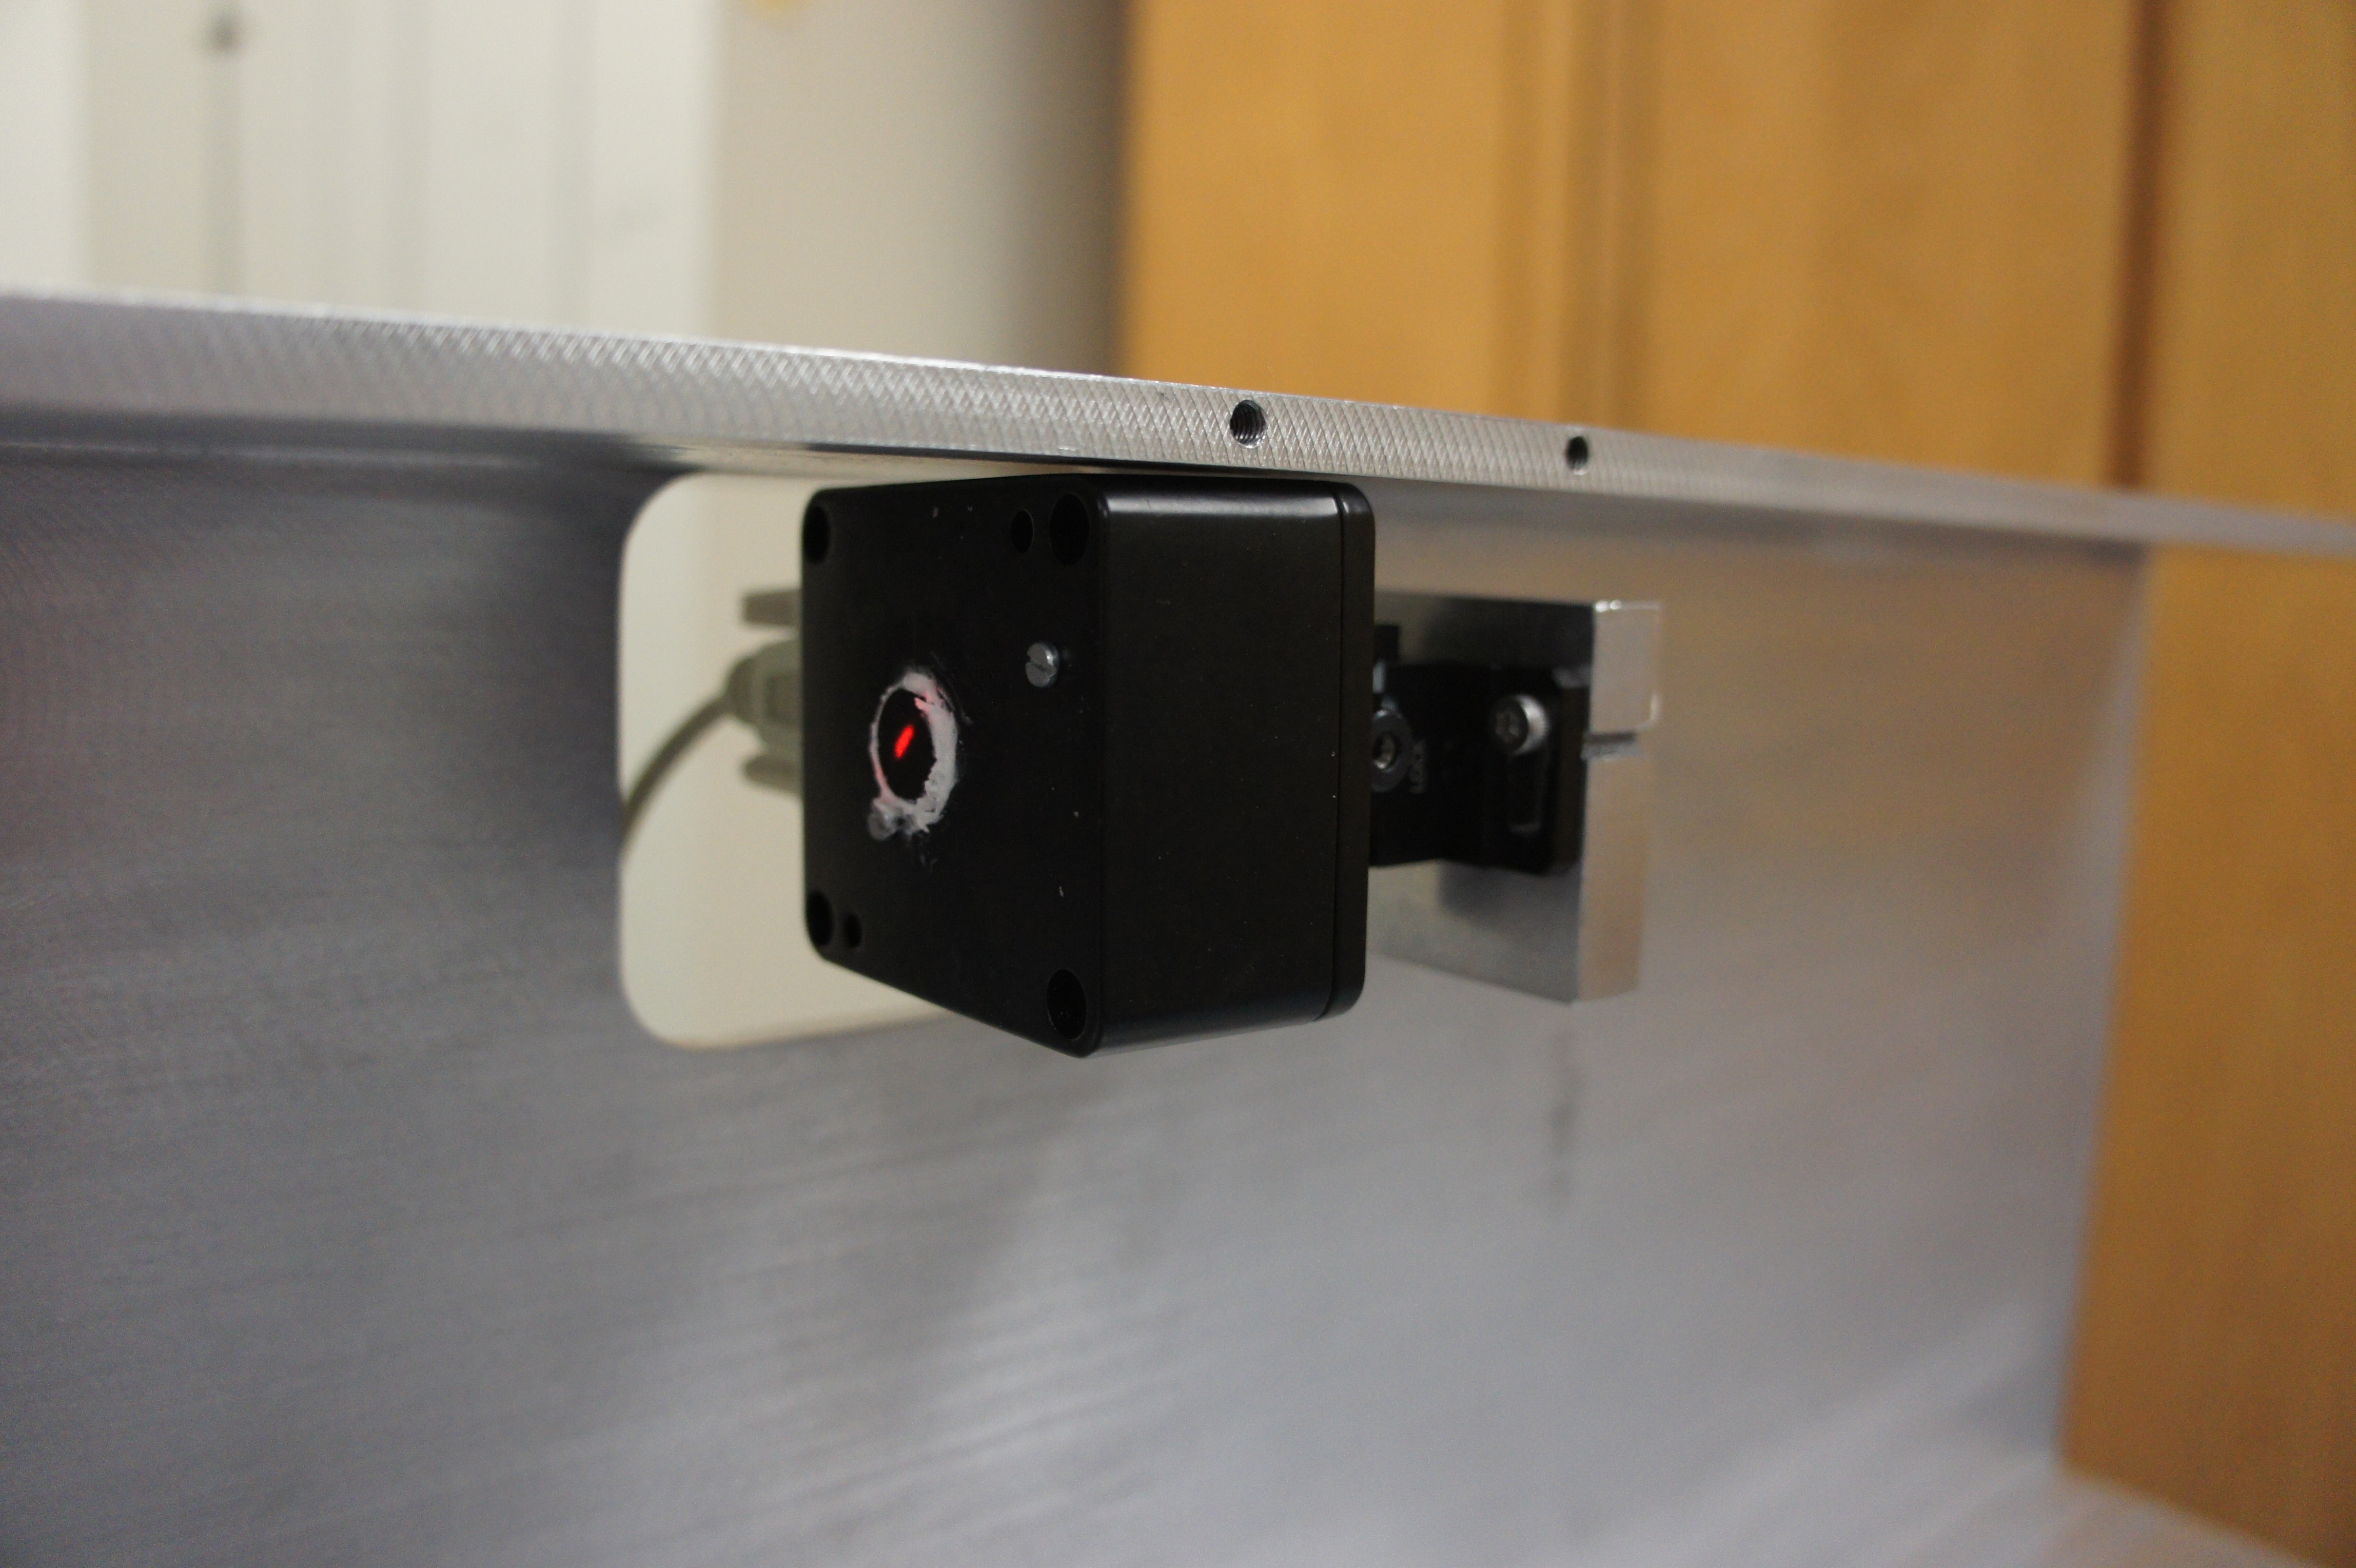
\includegraphics[width=4cm]{plots/qpd.jpg}
        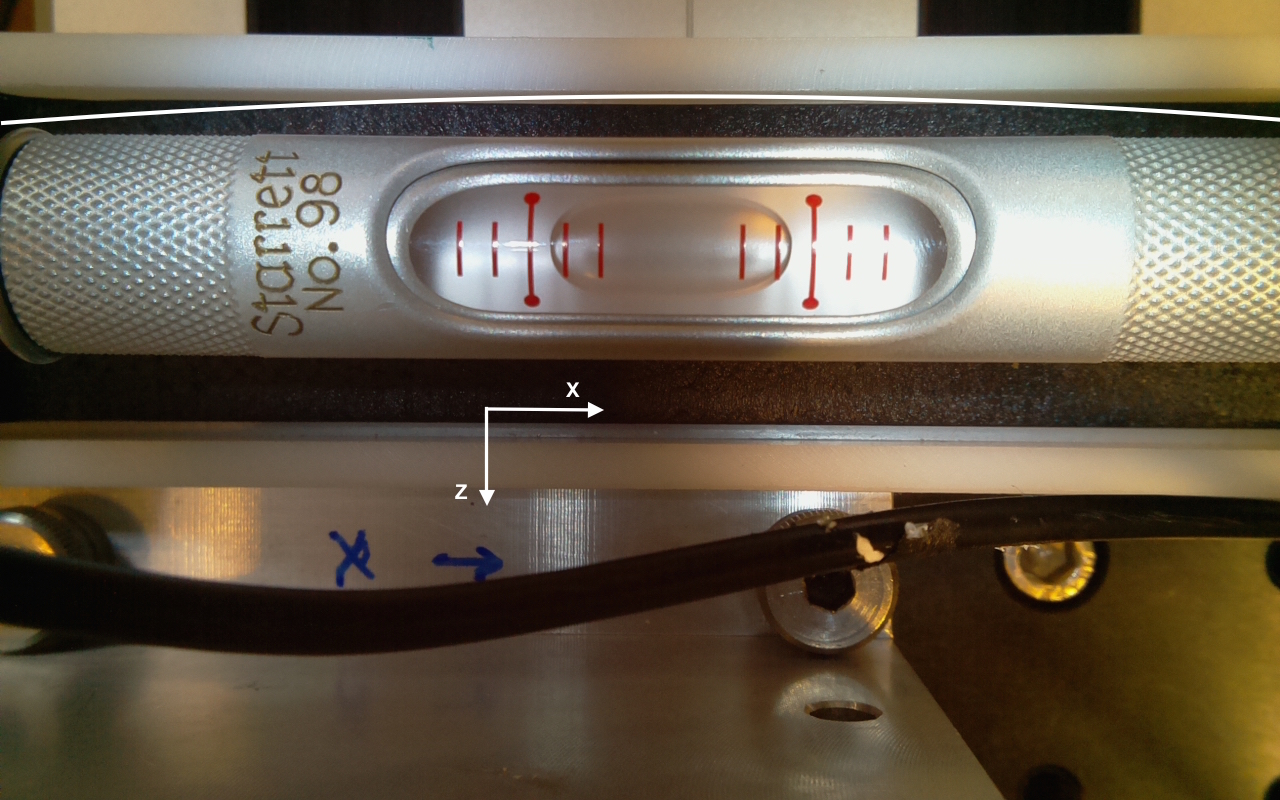
\includegraphics[width=4cm]{plots/whitetray.jpg}
      \caption{The quadrant photodiode (left) and the bubble level
                (right) for measuring rotations about the primary
                axes.}
      \label{fig:bubblelevel}
    \end{figure}  


      %%\subsection{Corrections to the beam position}
      %%
      %%%Relative angles measured by the bubble level are normalized to the
      %%%reference measurement made by the optical survey at the axial center
      %%%Z = 0 mm.
      %%Secondly, the rotation of the X-ray collimator about Z~axis 
      %%to the $\phi$ coordinate of the X-ray equal to the angle  of 
      %%rotation. 
      %%
      %%The $\phi$ correction ($\Delta \phi$) The rotation of the X-ray about
      %%Z-axis introduces a correction to the phi coordinate of the X-ray
      %%equal to the rotation angle.  The rotation about Z axis displaces the
      %%X-ray $\phi$ equal to the angle of rotation. Hence, angular
      %%measurement from the bubble level, calculated in the right-handed
      %%reference frame, is added to the nominal $\phi$. 
      %%
      %%Another correction to the X-ray $\phi$ is required due to radial offset between the center
      %%of rotation and the Another correction to the $\phi$ coordinate is required due based on
      %%the 
      %%The $\phi$ correction is given by the measured Z rotation and the phi offset 



      %A radial offset between the
      %center of rotation and the collimator requires a $\phi$ dependent
      %correction, maximally calculated to 0.38~mrad.


      %%\subsection{Uncertainties}
      %%\label{sec:corruncertainties}
      %%Variation in the relative intensities of the laser leads to
      %%uncertainty on the angular rotations about X and Y axes. The
      %%uncertainty on the Z correction is calculated as maximum
      %%deviation allowed by the variation of the rotation angles in their
      %%uncertainty ranges. 
      %%
      %%The Z correction varies as a function of Z and
      %%$\phi$ between $\pm$0.6~mm with an average uncertainty of 0.03 mm
      %%(10\%).  The uncertainty in the rotation angle about Z axis ($\zeta_z$) is
      %%determined as the change in the angle calculated from two consecutive
      %%runs. The $\phi$ correction due to a rotation about Z axis ranges
      %%from -0.3 to 0.3 mrad and average uncertainty 0.12 mrad (40\%).
      %%Figure~\ref{fig:unc} shows the correction to the nominal coordinates
      %%of X-ray beam with uncertainties.
      %%
      %%
      %%\begin{figure}[]
      %%  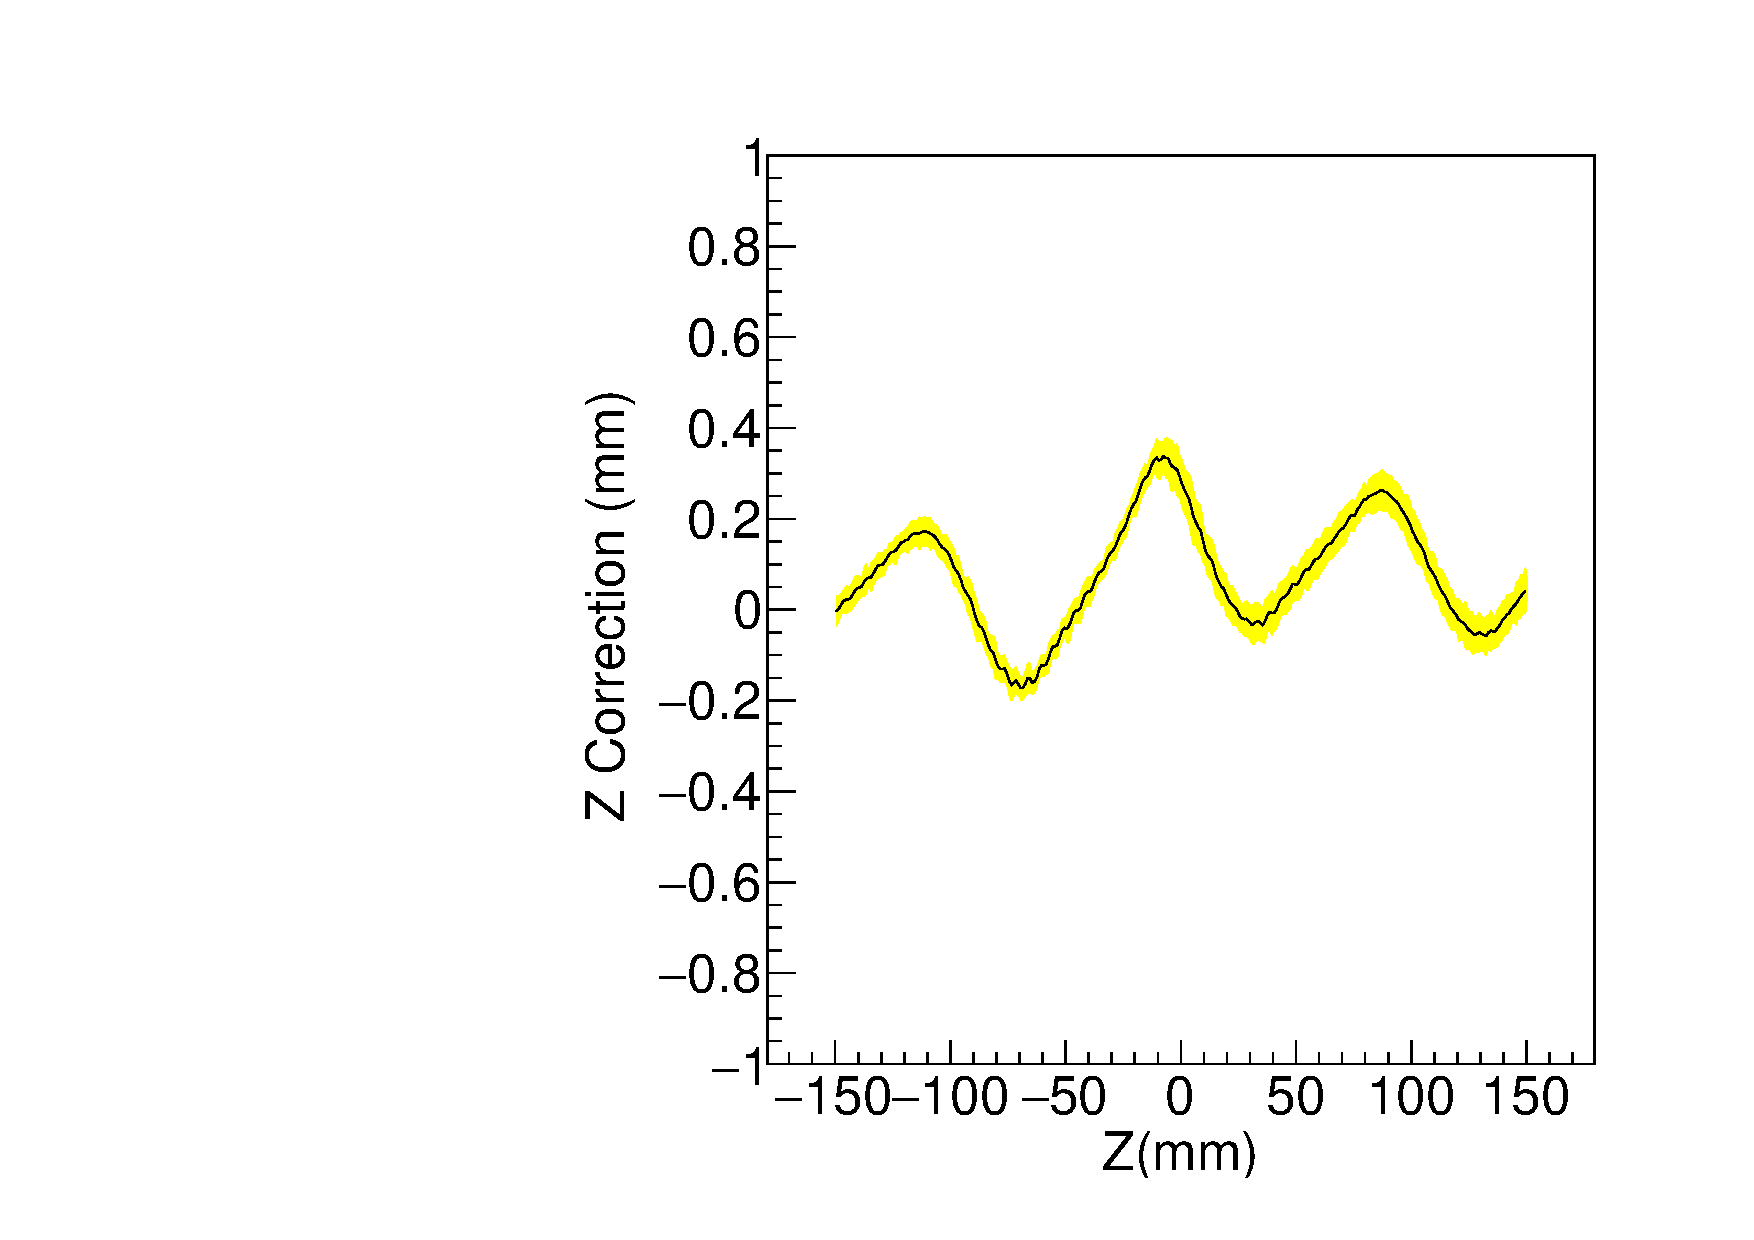
\includegraphics[width=7cm]{plots/cerr1}
      %%  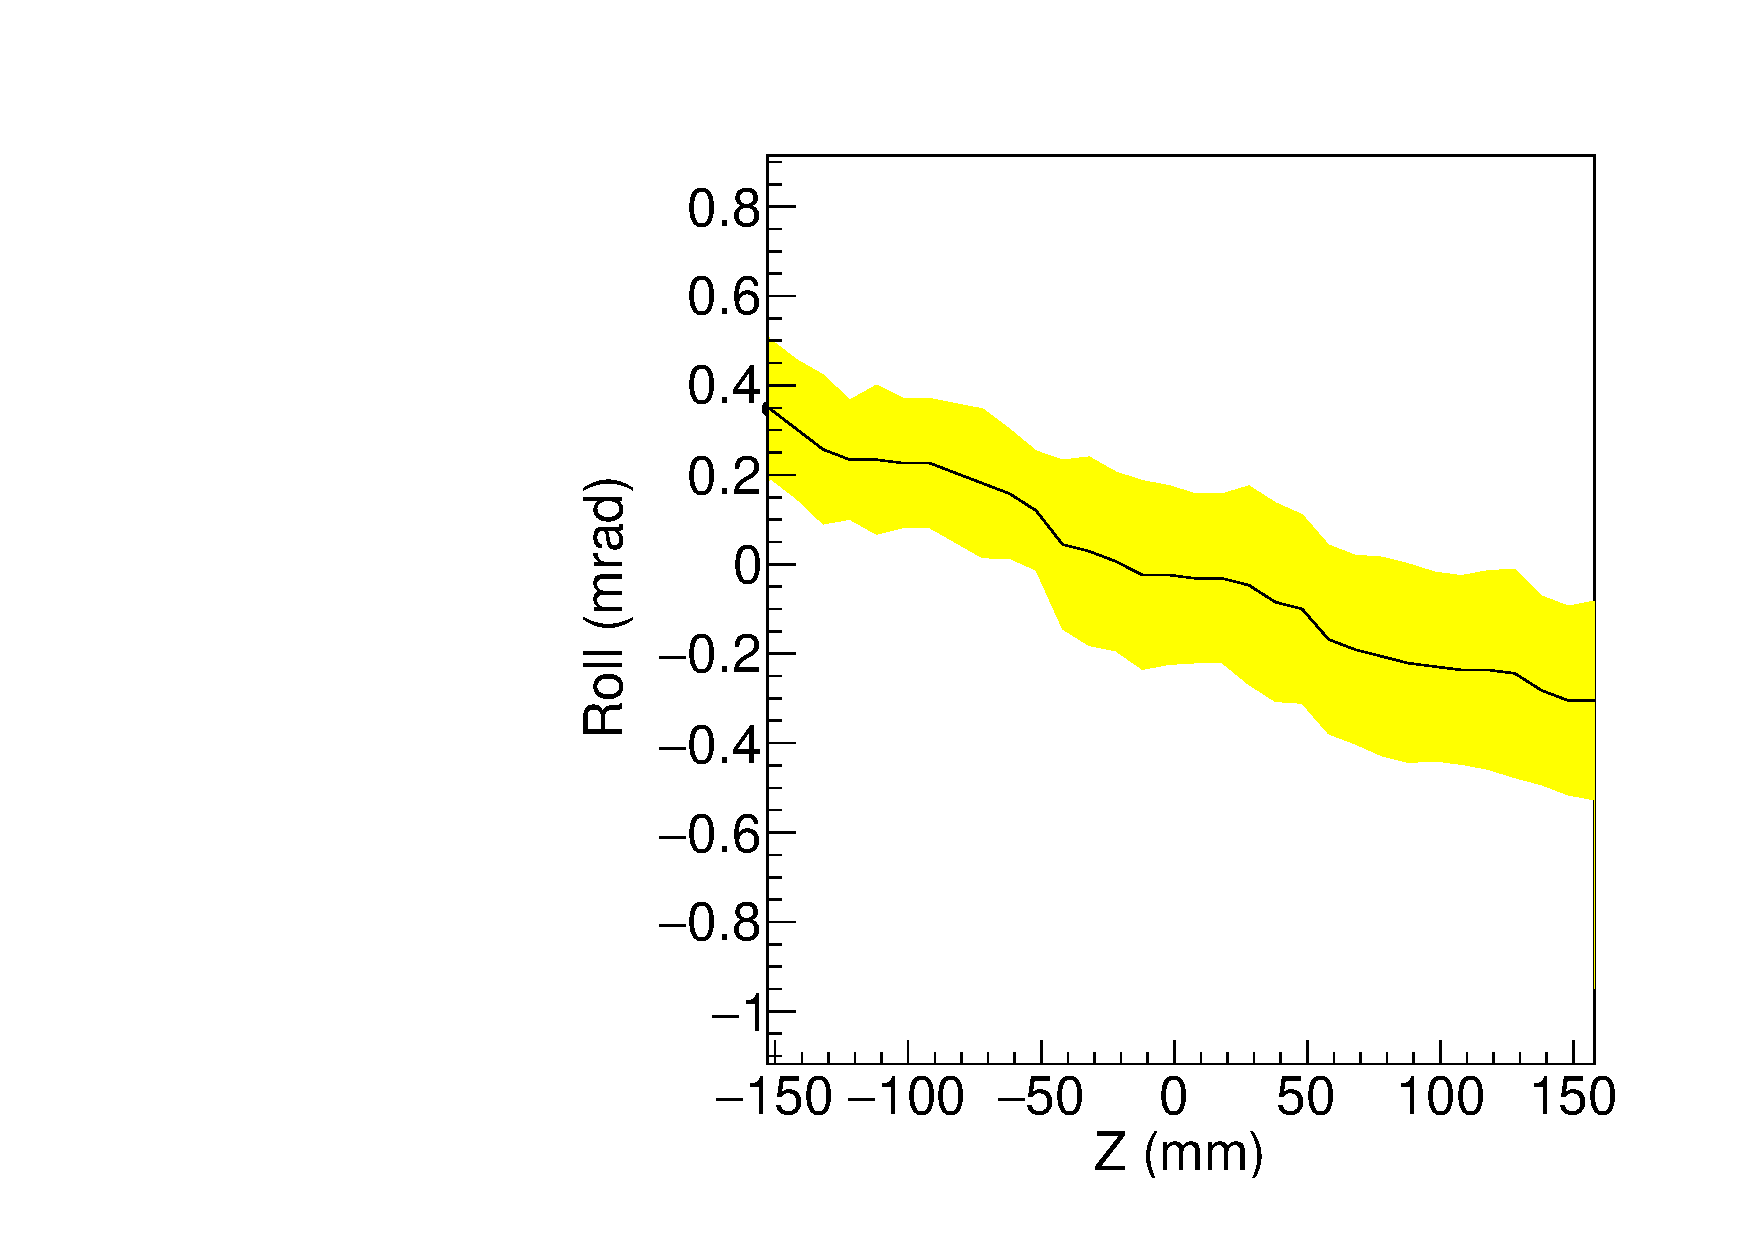
\includegraphics[width=7cm]{plots/rollUnc1}
      %%  \caption{Correction applied to X-ray coordinates Z and $\phi$ with
      %%  uncertainties.}
      %%  \label{fig:unc}
      %%\end{figure}  


\section{\label{sec5}Dataset}
The X-ray survey was performed twice, in 2017 and 2018.  In 2017,
single channel trigger used due to limited readout capacity of
DAQ was susceptible to coherent noise and cosmic backgrounds. As a
result, signal to background ratio of $\sim$1 was attained.  The
following year an upgraded DAQ with full waveform data facilitated a
more complex trigger capable of identifying
cosmic rays and noise events, which improved the signal to backgorund ratio
to 12.

The X-rays are absorbed by the magnetic coils (in COBRA) and the
liquid Xe scintillator.  Monte Carlo simulation of the magnet
estimated the absorption of 70\% and was confirmed by LYSO
scintillator crystals placed inside and outside the magnet in the path
of the X-rays (Figure~\ref{fig:absorption}). The absorption in the
calorimeter due to liquid Xe is dependent on the X-ray absorption
length in Xe ($\lambda_{\mathrm{Xe}}$ = 2.9 mm) and the radial
thickness of Xe column traversed by the X-ray before showering.  The
installation of the MPPCs on the cryostat wall makes it unlikely that
any liquid Xe can accumulate behind the MPPCs\cite{megdesign}.
Therefore, loss in signal due to such interactions is expected to be
small.  The normalized rate of X-ray decays observed as a function of
radial distance is shown in figure~\ref{fig:absorption}.

\begin{figure}[]
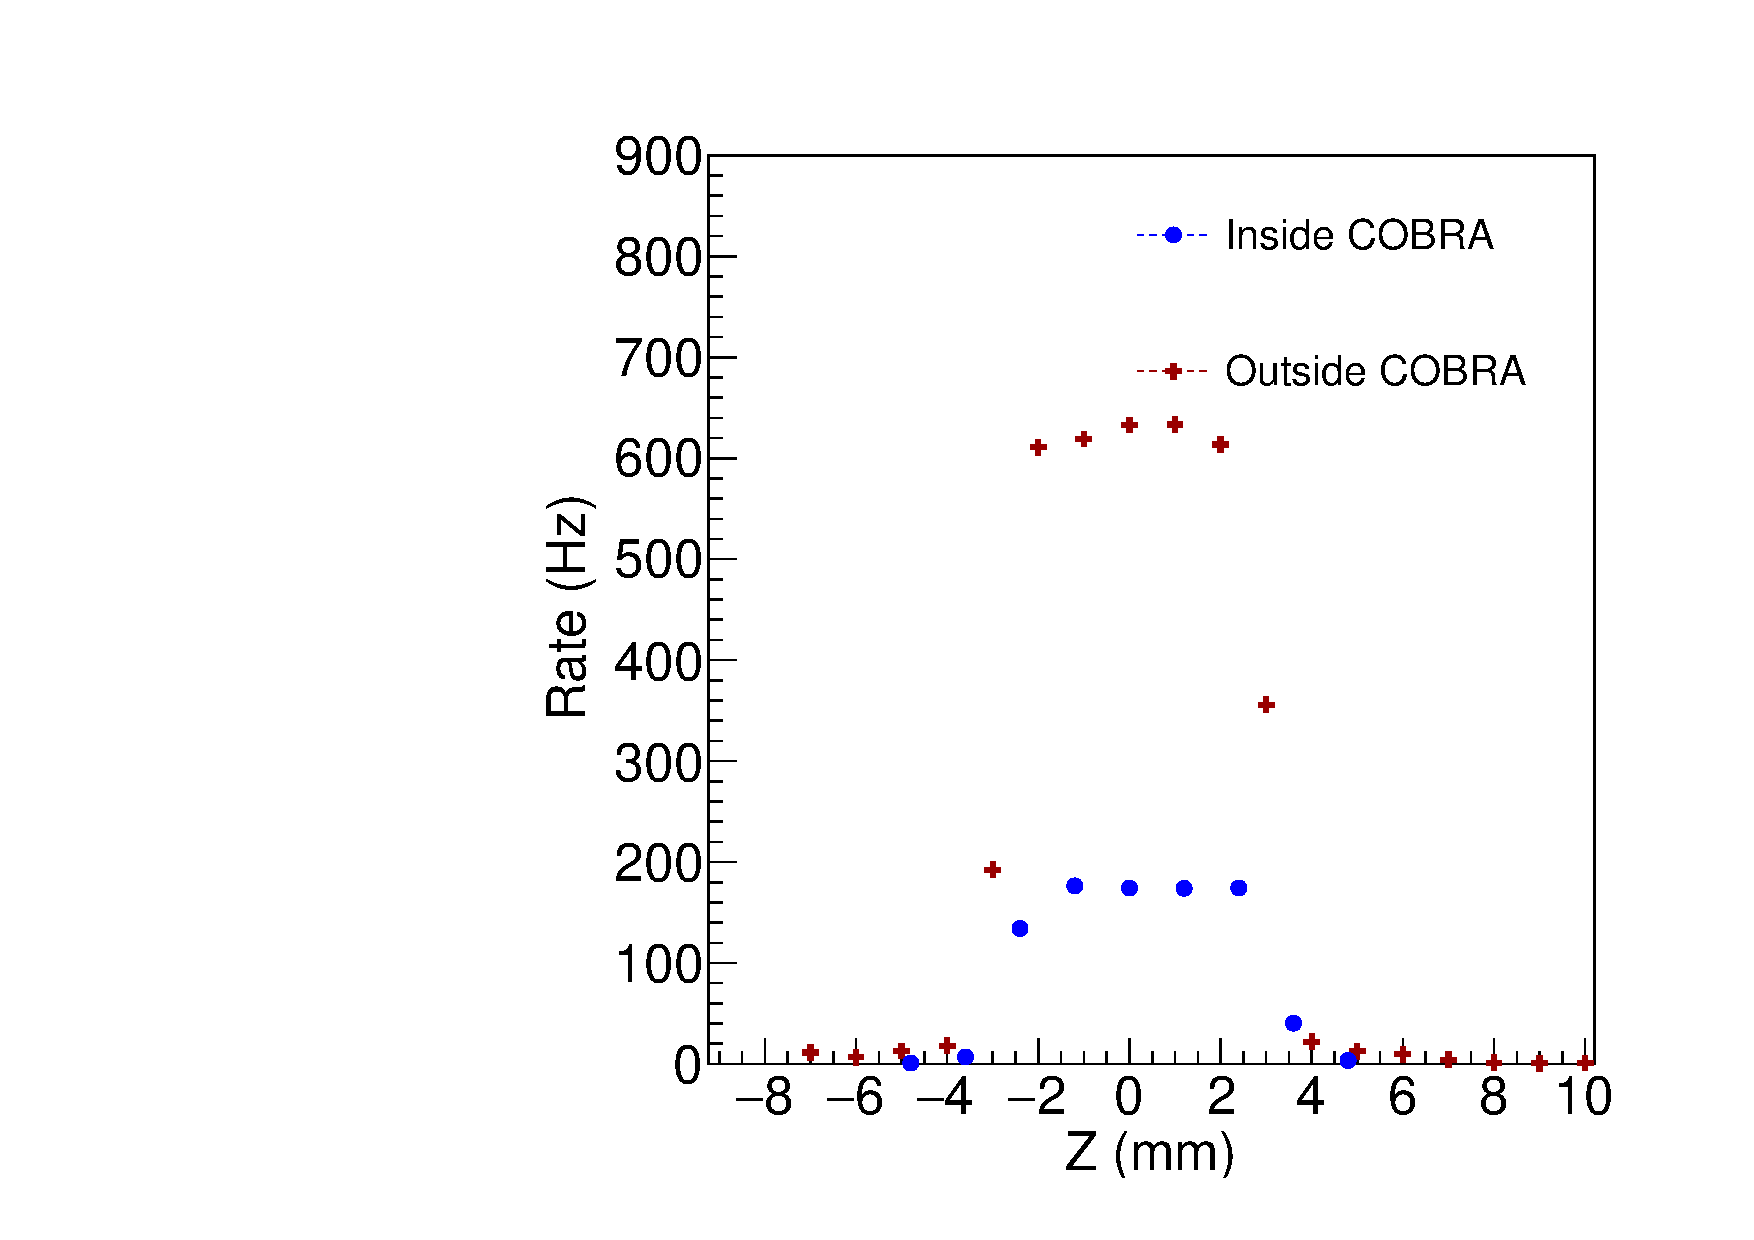
\includegraphics[width=4cm]{plots/xray_cobra_absorption}
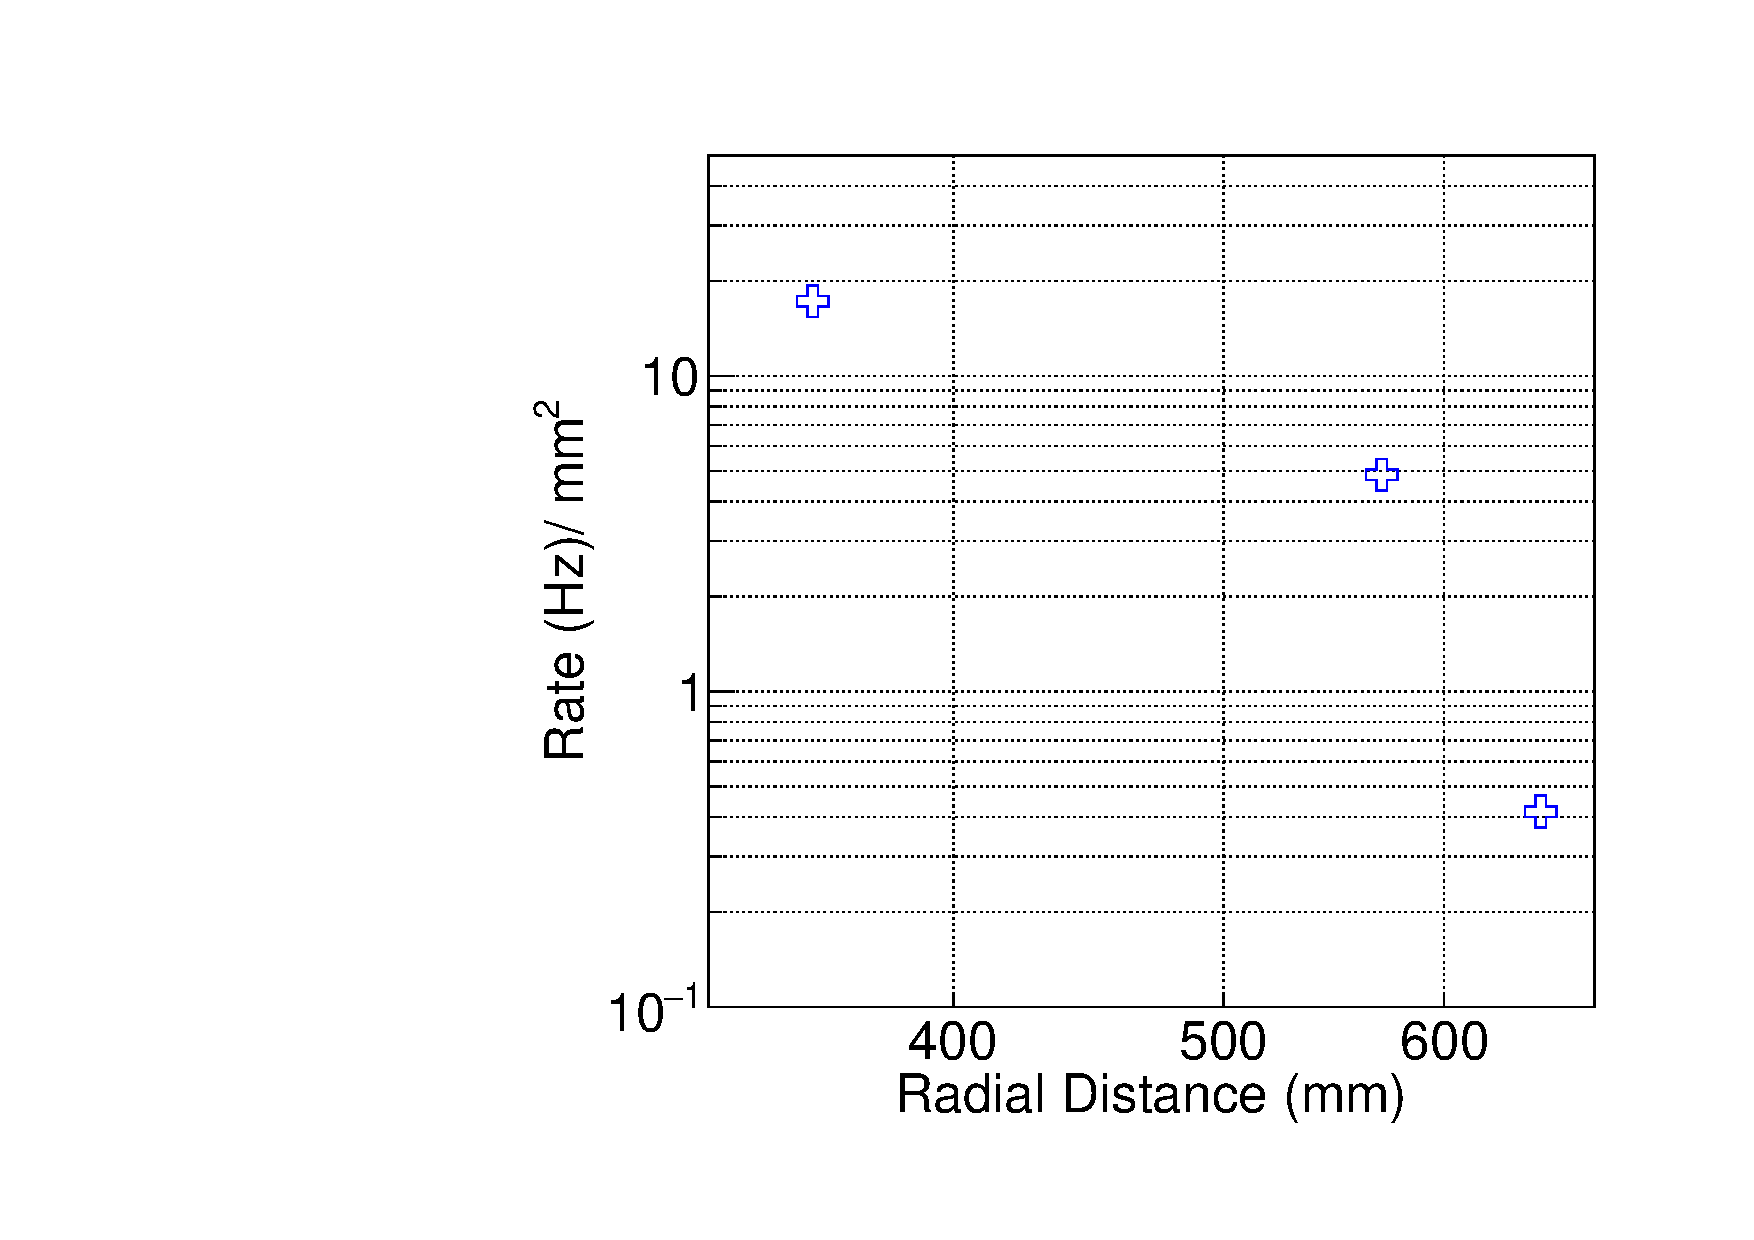
\includegraphics[width=4cm]{plots/rate_vs_radius} 
\caption{X-ray
interaction rates in LYSO scintillator inside and outside COBRA magnet
(left) and normalized interaction rate as a function of radial
distance (right).} \label{fig:absorption} 
\end{figure}  


%\subsection{Scan Summmary}
The collimator projects a thin beam on the inner face of the cryostat
fully covering two MPPCs simultaneously in the long direction.  The Z
and $\phi$ coordinates of the MPPCs are scanned separately, each using
the long-edge of the collimated beam in the vertical and horizontal
orientations respectively.
Collection from a non-scanned span of two MPPCs, adjacent in the long direction, is used for rejection of background events.
Data is collected with the scanning step of
1~mm (0.08~deg) in Z ($\phi$) direction.  Increase in the material
cross-section outside the axially central region ($|$Z$|>$120 mm)
causes enhanced absorption of the X-rays making the calorimeter nearly
opaque to the X-ray scan (Figure~\ref{fig:ratevsz}).  Hence, the scanning
region is restricted in $|$Z$|<$120~mm and covers the entire range in
$\phi$, $120\degree<\phi<\,240\degree$.  In 2017, the full set of the
accessible MPPCs about 46\% (1900 of 4092) were scanned; a subset of
these, about 700, were scanned again in 2018.

\begin{figure}[] 
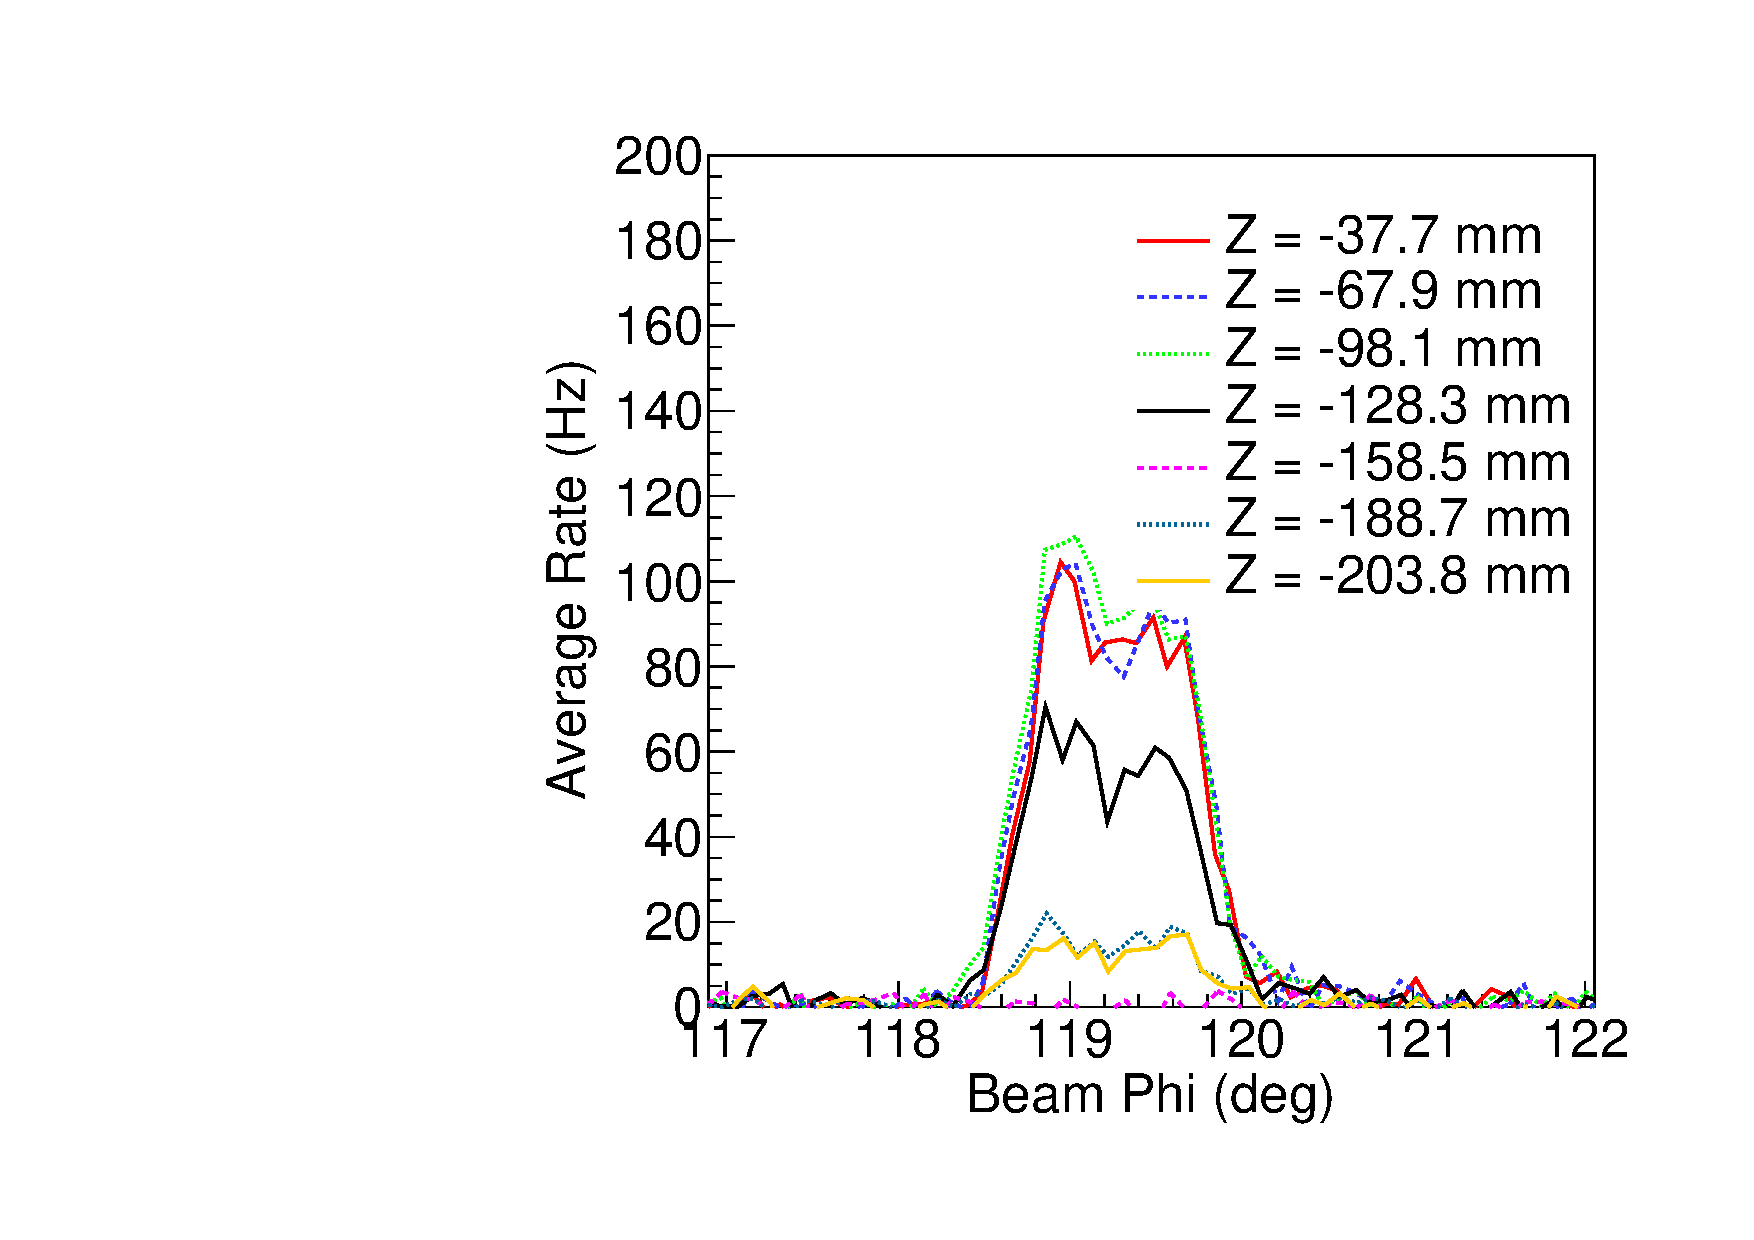
\includegraphics[width=4cm]{plots/xray_vs_Z}
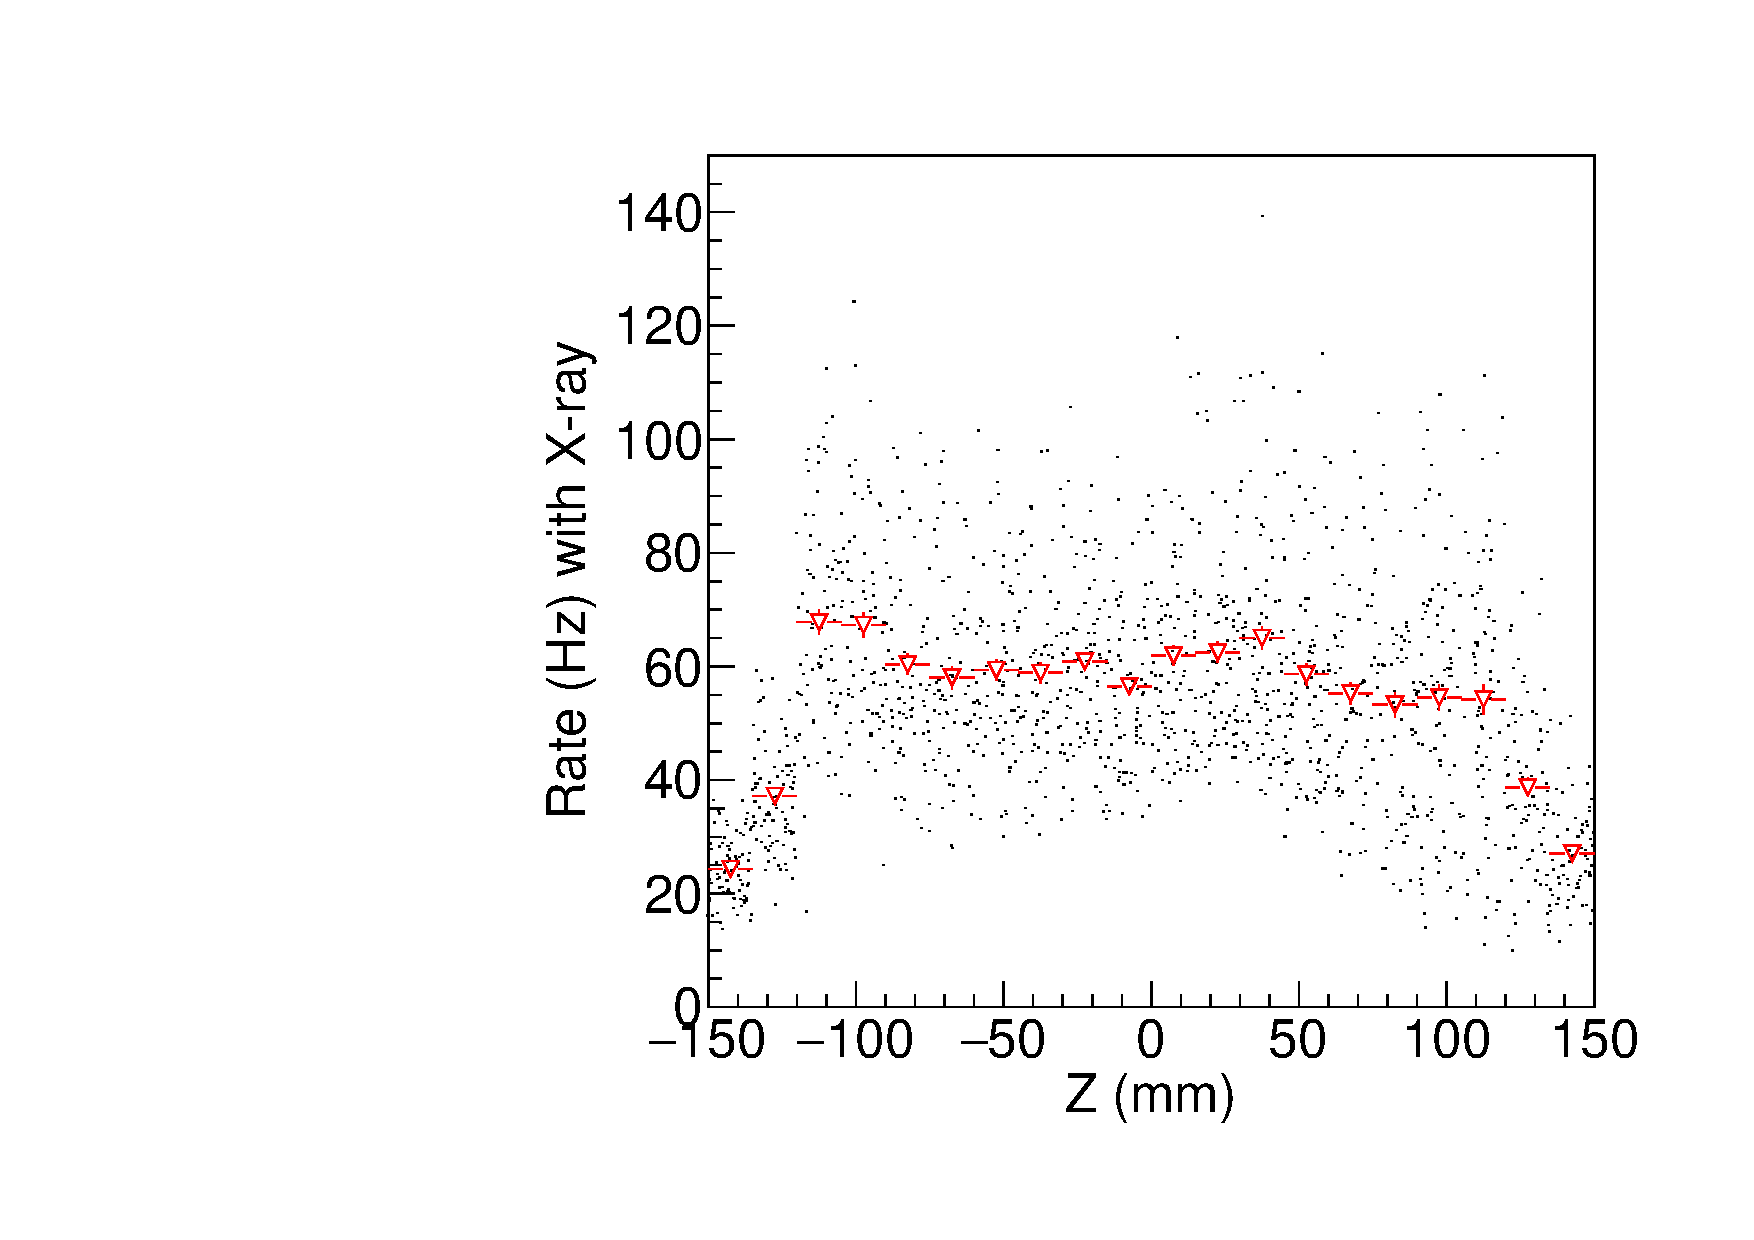
\includegraphics[width=4cm]{plots/csig_z_phiscan} \caption{Drop in
observed X-ray interactions as a function of axial (Z)  location.}
\label{fig:ratevsz} 
\end{figure}  


%%\begin{figure}[]
%%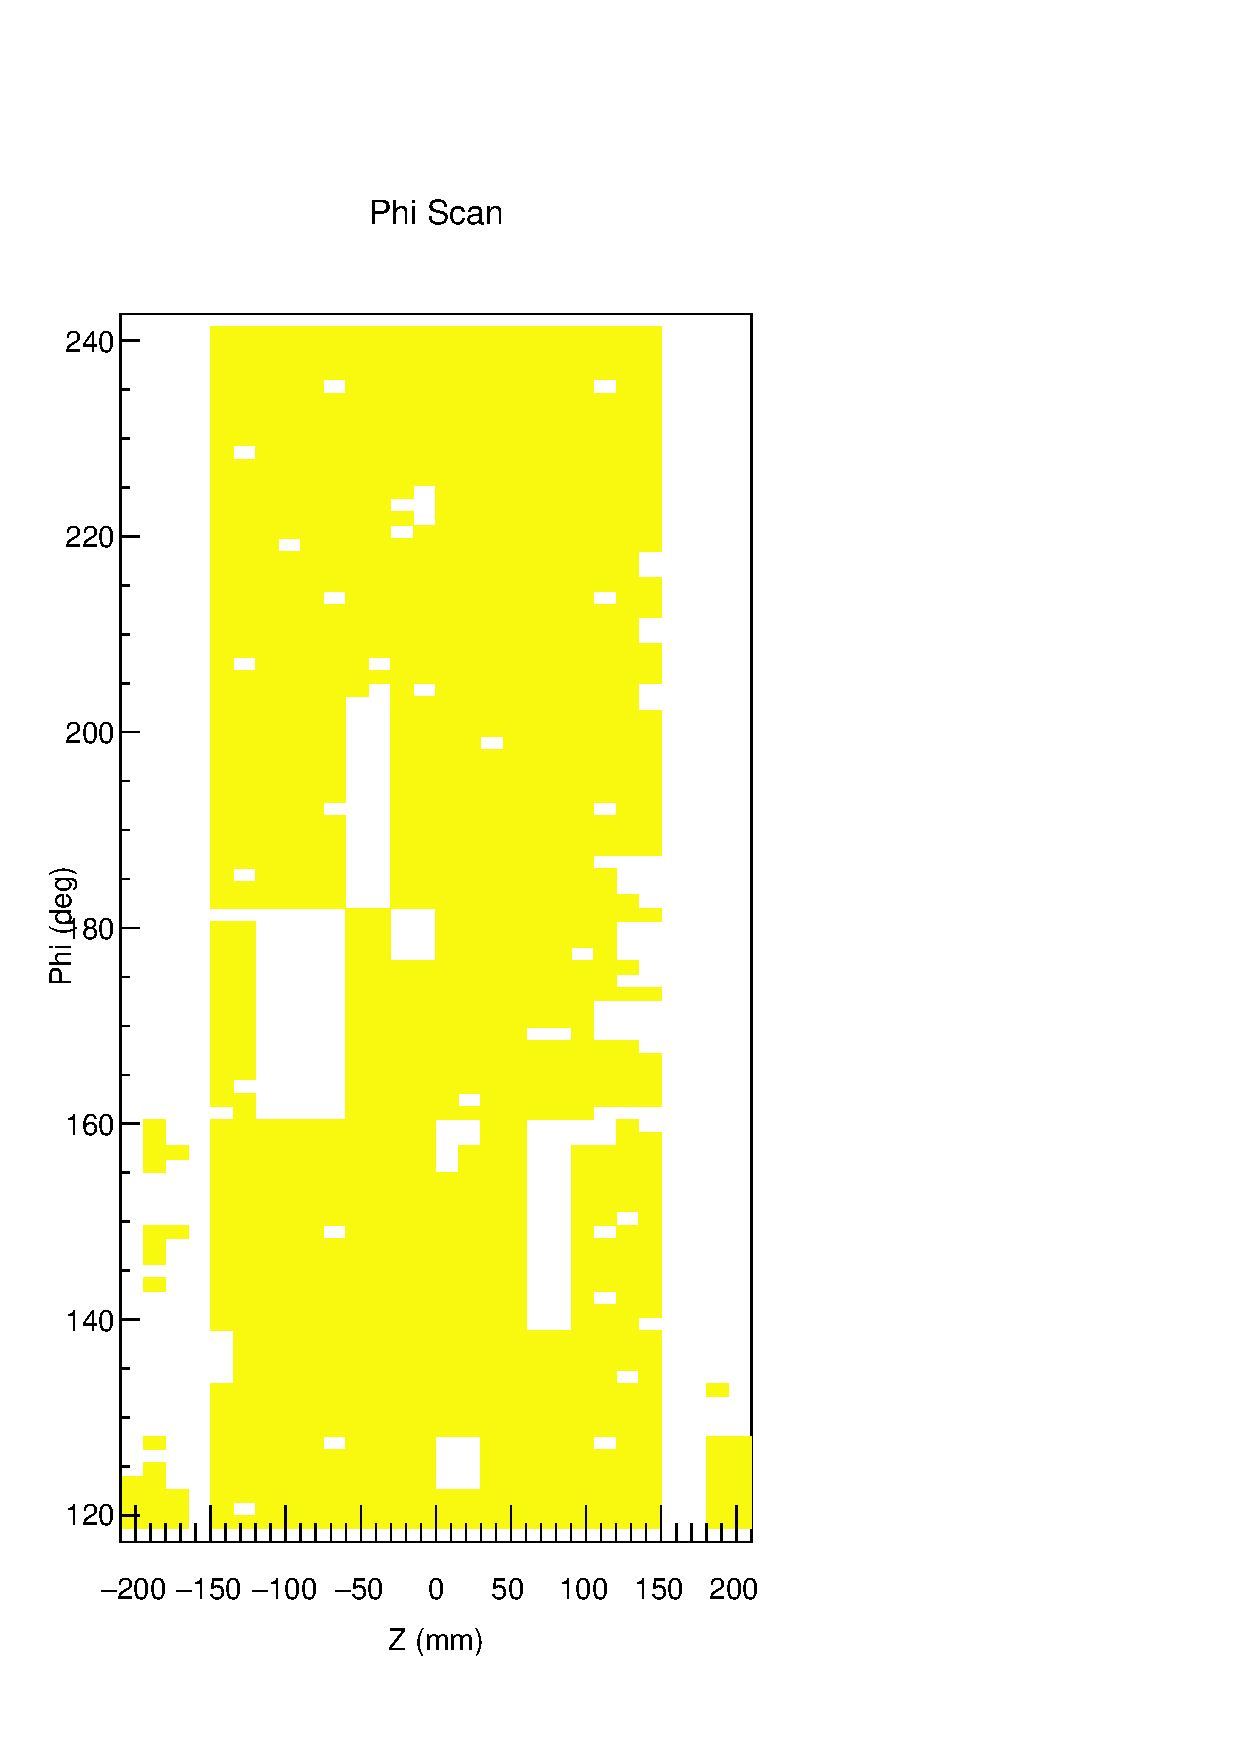
\includegraphics[width=7cm]{plots/c2_phi}
%%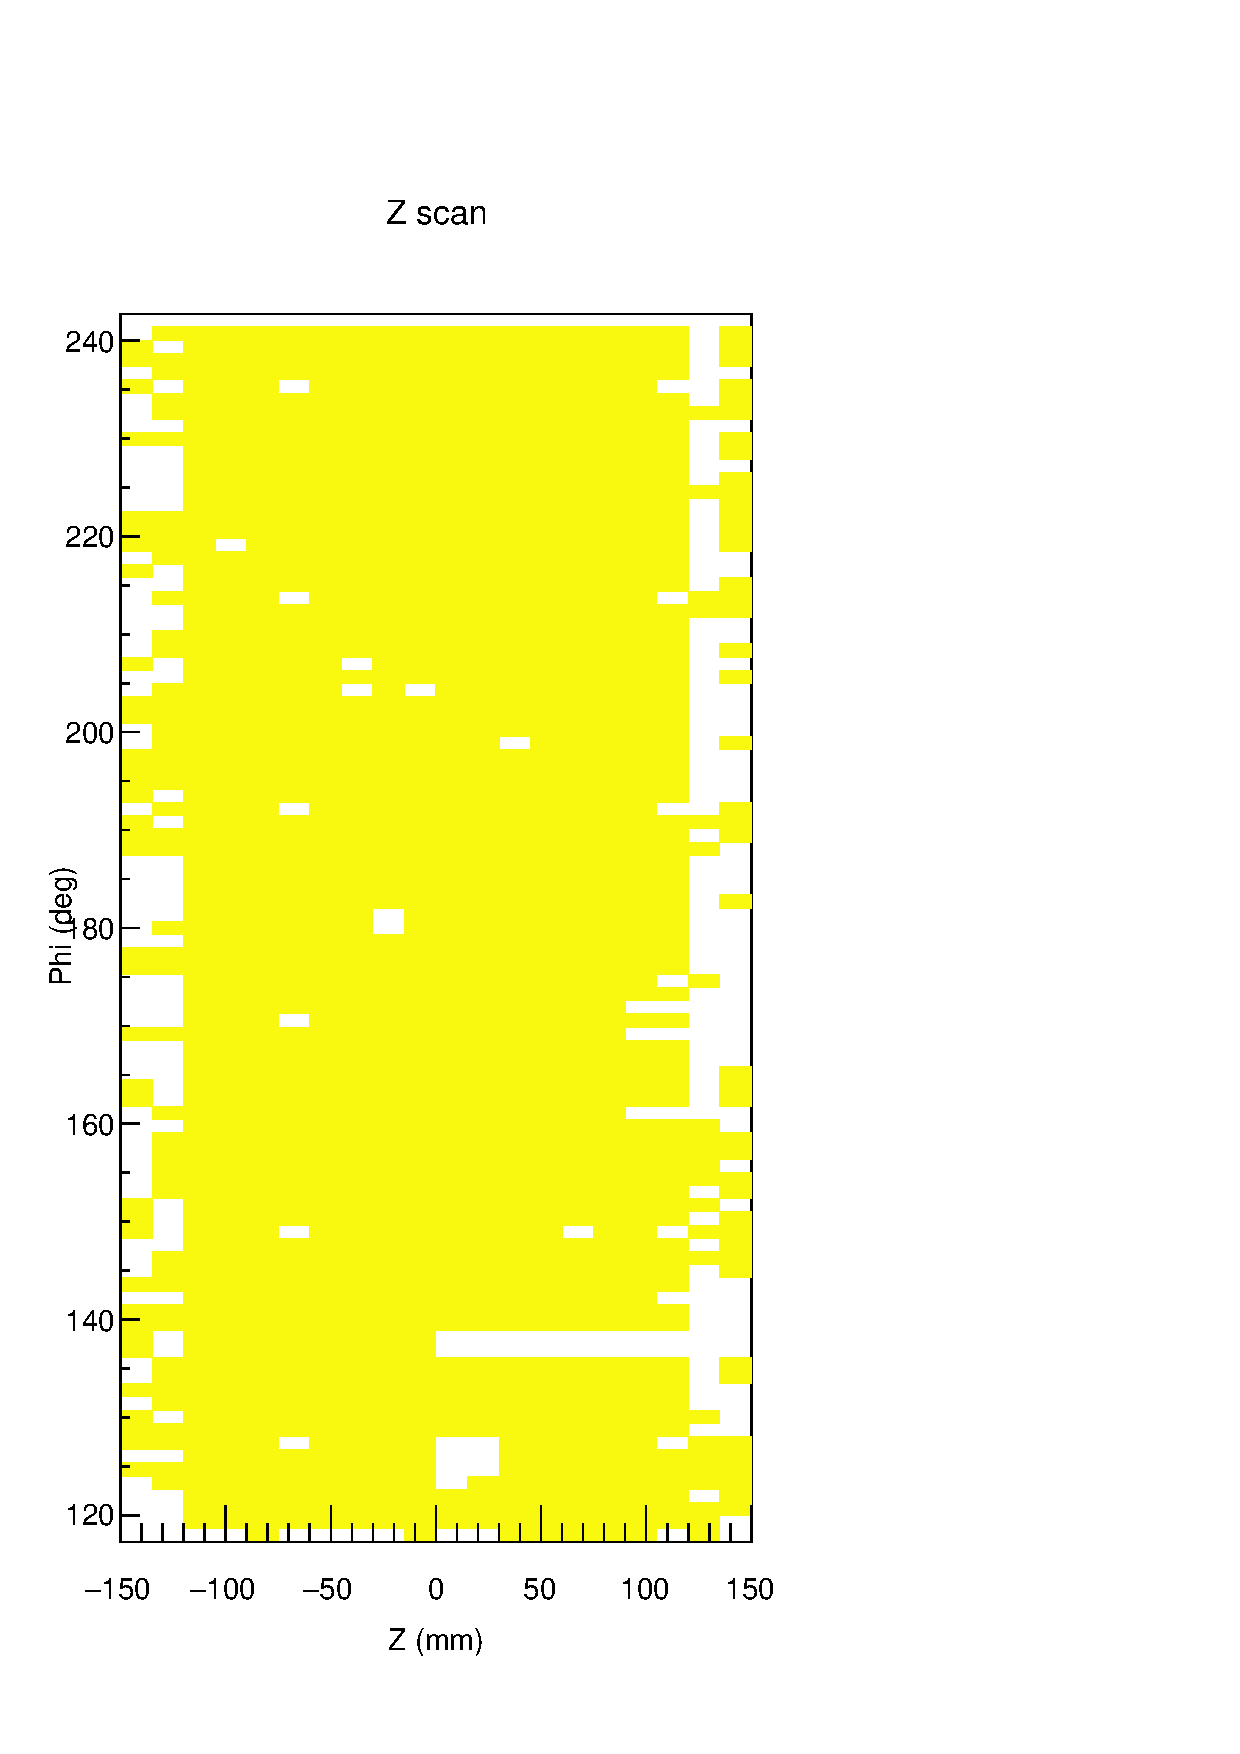
\includegraphics[width=7cm]{plots/calc-all}
%%\caption{Scanned MPPCs for $\phi$ and Z coordinates after quality cuts.}
%%\label{fig:scanmap}
%%\end{figure}  



\section{Photodetector position}\label{sec:mppcposition}
The location of each photodetector is determined using charge
generated in the photodectectors by X-ray interactions corresponding
to a precisely placed source.  An outline of the detector is created
by X-ray events and fitted to determine the center position (fig
\ref{fig:xrayevents}). 

\begin{figure}[h]
  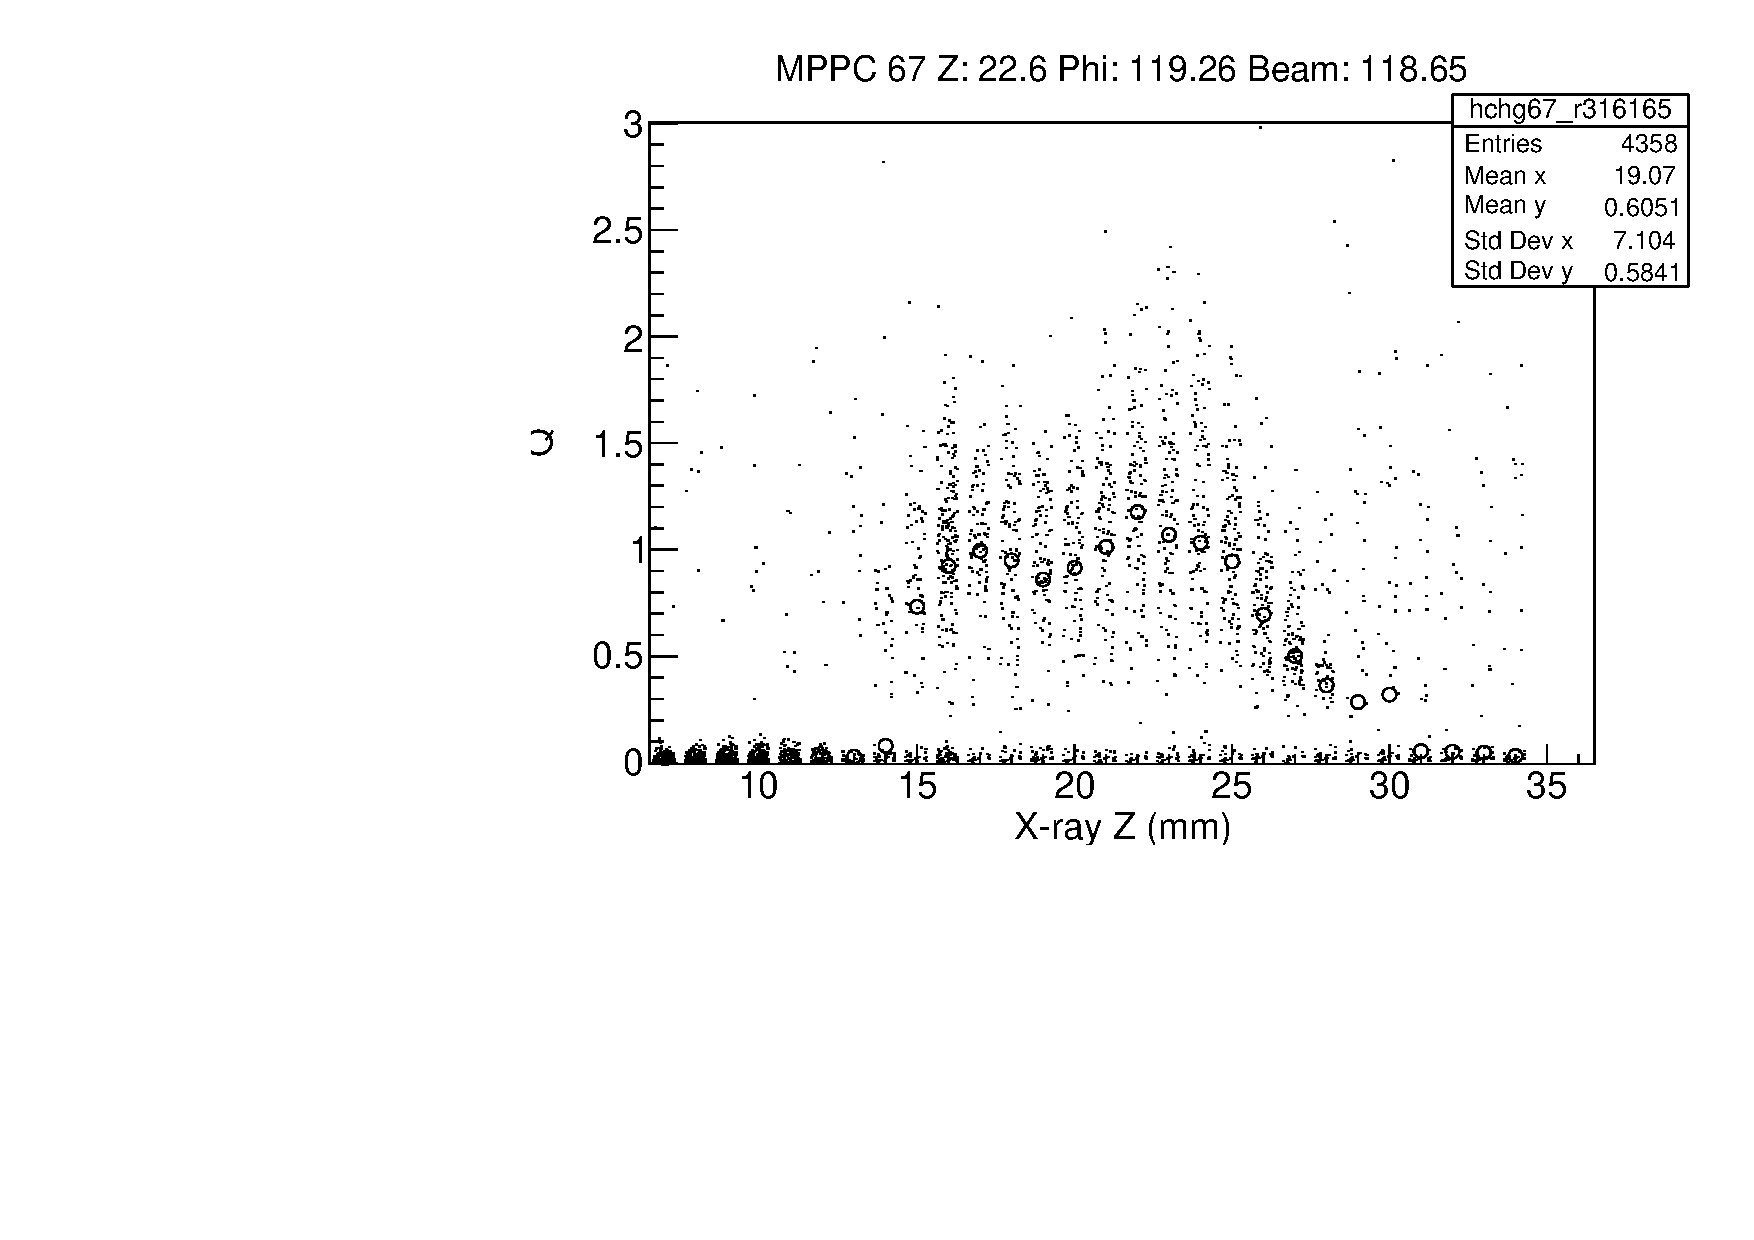
\includegraphics[width=4cm]{plots/2018/hcharge67_z}
  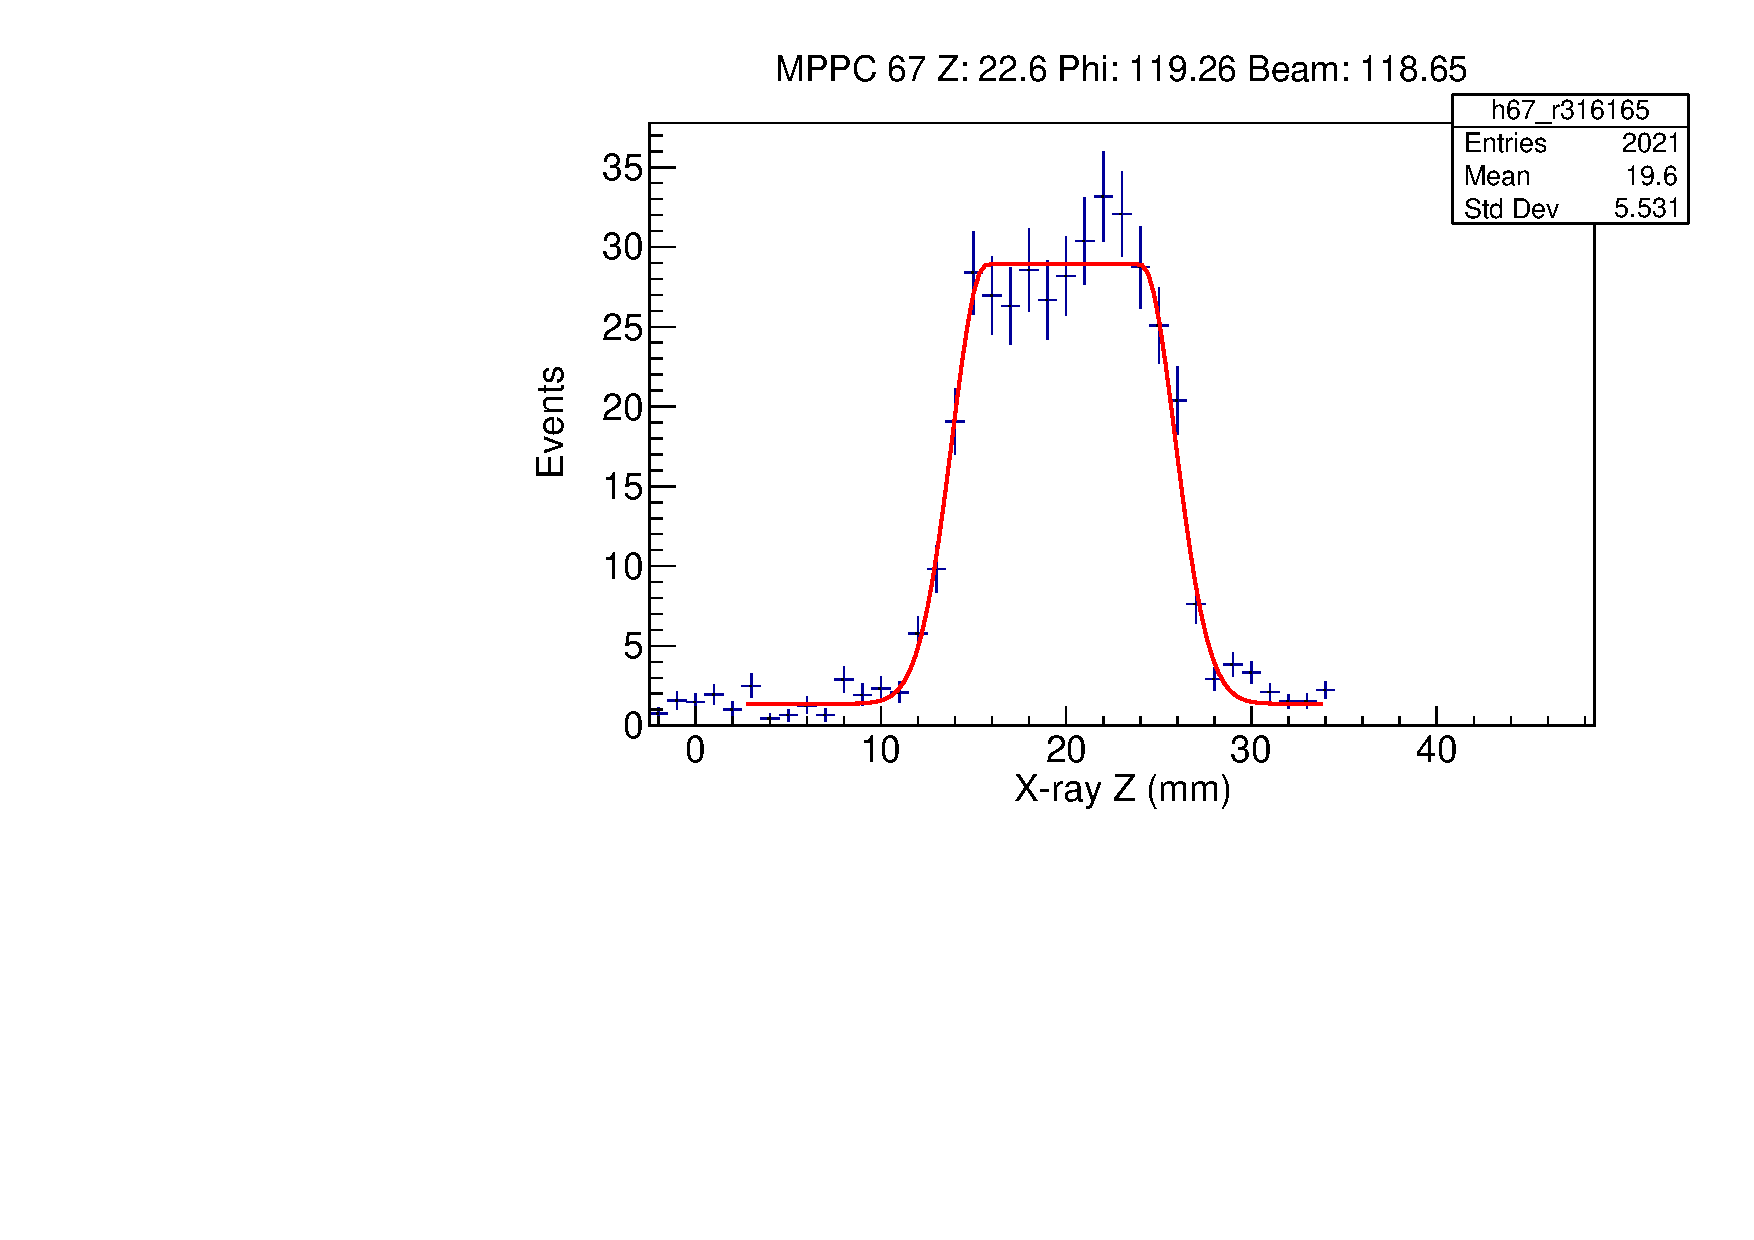
\includegraphics[width=4cm]{plots/2018/mppc_fit}
  \caption{Charge recorded in a single photodetector as a function of X-ray Z coordinate 
  (left) and 
    the calculated event rate (right).}
  \label{fig:xrayevents}
\end{figure}  

To isolate signal events, a trigger threshold on cumulative charge 
in the region of scanned photodetectors is applied with background 
subtraction to exclude coherent electronic noise. Additionally, 
an offline selection criteria matching X-ray energy pattern are applied
requiring large relative and absolute charge in the channel with highest charge
($>70\%$, $>0.4$~pC), and simulataneously a small deposition 
in the channel with the second highest charge ($<10\%$),
and rest of the channels ($<0.1$~pC).

The X-ray event rate as a function of X-ray position ($z/\phi$) is
fitted with the following peicewise continuous function,\\
\begin{math}\label{eqn:mppcfitfcn}
f(z) = 
\begin{cases}
   b+s\cdot 
Exp\left[-\frac{(z - \, (\mu_m - w/2)\,)^2}{\sigma_m^2}\right] & z <
\mu_m-w/2  \vspace{3mm} \\
   b+s\cdot 
Exp\left[-\frac{(z - \, (\mu_m + w/2)\, )^2}{\sigma_m^2}\right] & z >
\mu_m+w/2    \vspace{3mm} \\
   b+s                                         & \mu_m - w/2 < z < \\
                                               & \mu_m + w/2    \\
\end{cases}
\end{math}

\noindent where, $w$ and $\mu_m$ are the width and center position of
the photodetector, $\sigma_m$ gaussian width of the edges, and $s,\,b$
are the signal and background event rates. A sample of well fitted
photodectector locations is used for  subsequent analysis.

The X-ray scans together with the fitted radial coordinate (described
in the next section) provide a 3D
location of each scanned photodetector  with high precision
($\sigma_{|\vec{x}|}<0.5$~mm).  These measurements are compared to a set of
nominal positions in the designed detector in order to reveal changes due to
manufacturing and installation.  Secondly, the two X-ray  measurements are
fitted to find global offsets in the absolute positions which could be
introduced due to the movement of the calorimeter or thermal cycling of LXe
scintillator conducted between the two scans.

The nominal positions of the photodetectors ($Z_{MPPC}$,
$\phi_{MPPC}$) are in a regular grid along a cylindrical surface with
constant radius, and its central axis aligned with the Z axis of the
MEG coordinate system.  From direct measurements in FARO and X-ray
surveys (described in the next section), we have shown  that the
radial coordinate of the photodetectors is not perfectly uniform.  We
find that the calorimeter can be divided into four separate regions
formed by the cfrp plates. Within each plate there is rotation of the
photodetectors about the radial axis which causes $\phi$ dependent
variation in the Z coordinate, and corresponding and equal Z dependent
variation in the $\phi$ coordinate of the MPPC measured by the X-ray
scan (figures \ref{fig:rotation1}, \ref{fig:rotation2}). The deviation of the measured from
the nominal in Z and $\phi$ coordinates is fitted independently on
mutiple subsets of photodetectors within each cfrp plate. The results
(table \ref{tab:rotation}) show the mean slope due to the rotation
varies between 2-5~mrad  or 1-4~mm displacement of the photodetector
over the entire calorimeter.
A consistently higher slope of  $d\phi/dZ$ compared to $dZ/d\phi$
indicates a 1~mrad deviation in the construction of the cfrp plate
from a perfectly 
rectilinear assembly board in the z-$\phi$ plane.  The figures and the
table show calculations using 2017 data, the results from the smaller
2018 data are found to be identical but not used. 

\begin{table}
\begin{tabular}{ccc}
   & $dZ/d\phi_{MPPC}$ & $d\phi/dZ_{MPPC}$ \\
\hline 
cfrp 1 & -0.0025 & 0.0033 \\
cfrp 2 & -0.0032 & 0.0040 \\
cfrp 3 & -0.0033 & 0.0045 \\
cfrp 4 & -0.0050 & 0.0058 \\
\end{tabular}
\caption{Average slopes (mm/mm) of deviation between X-ray and nominal MPPC positions
$dZ, d\phi$ with respect to the other coordinate, shown for each 
cfrp plate.}
\label{tab:rotation}
\end{table}

\begin{figure}
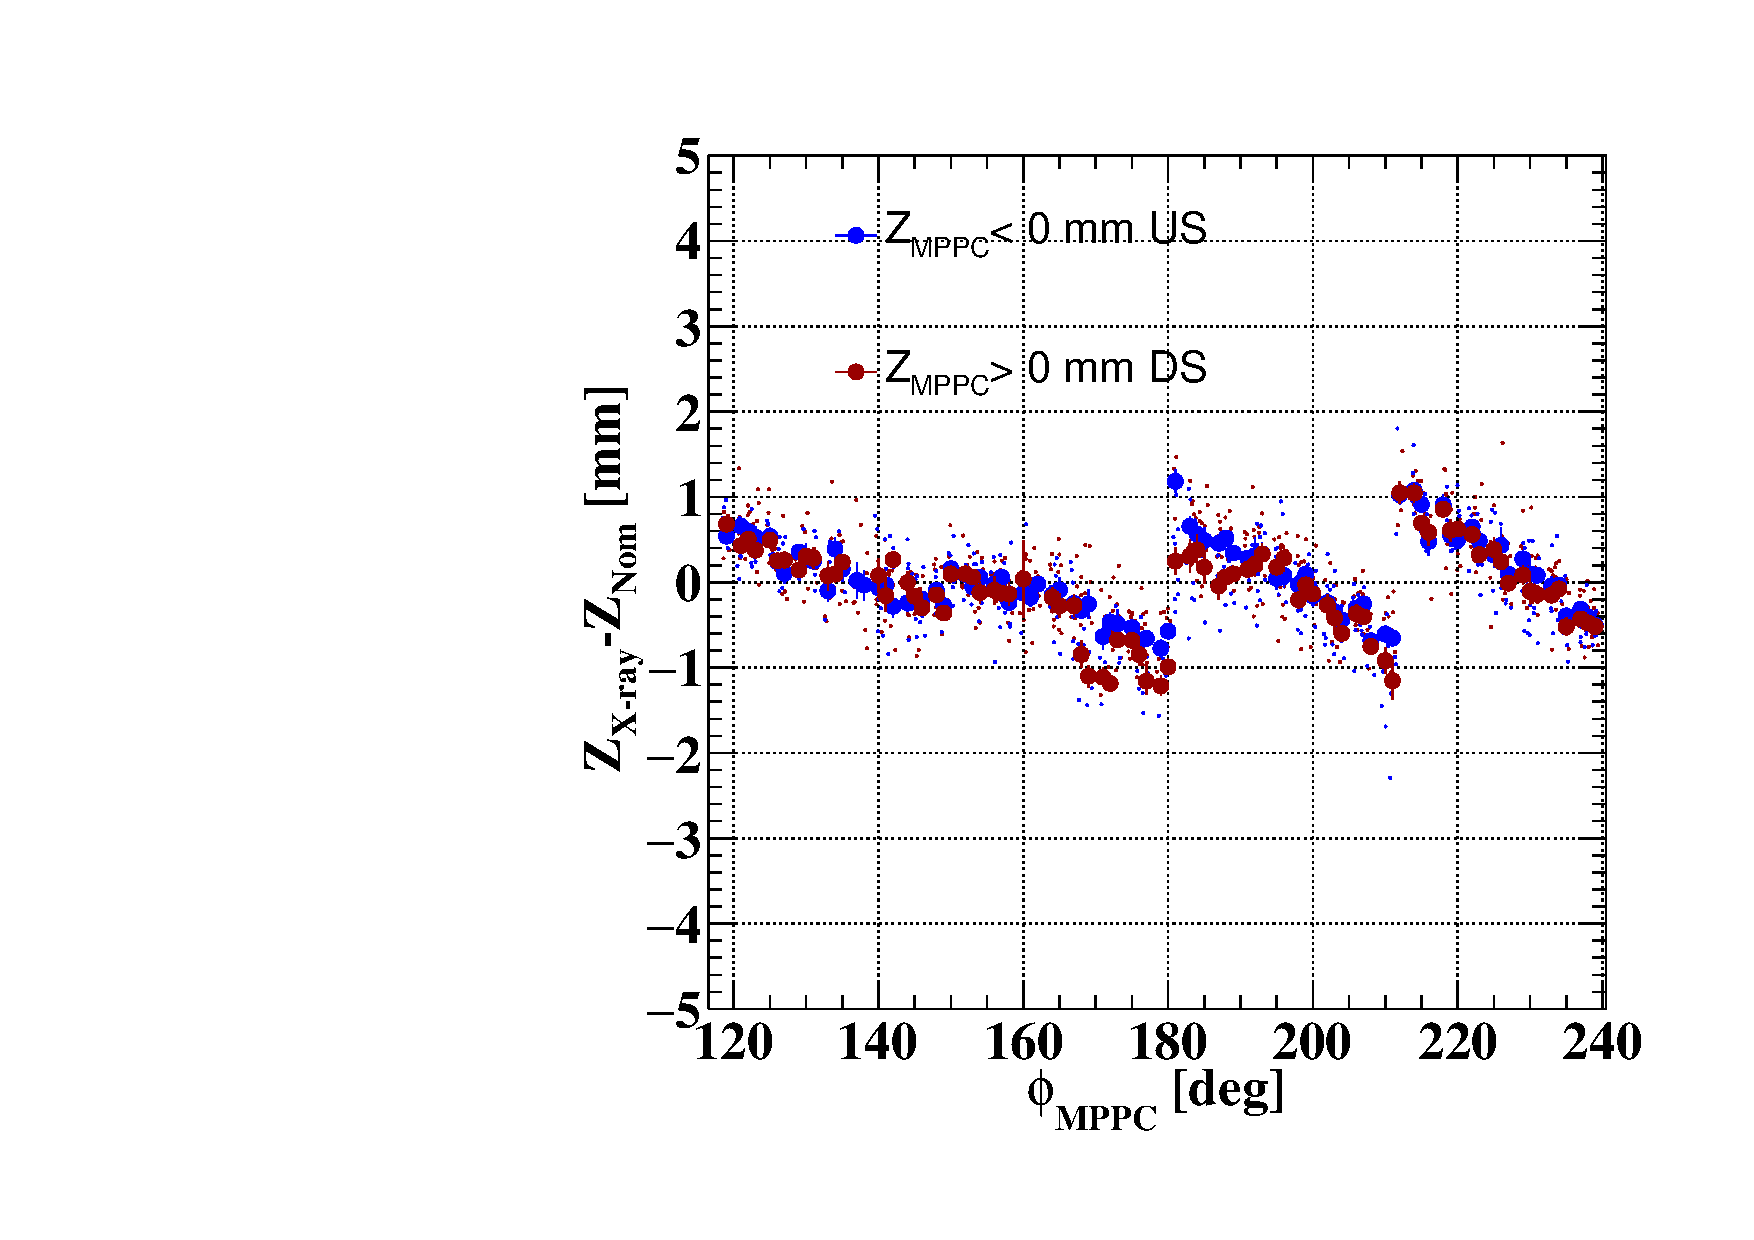
\includegraphics[width=4cm]{plots/dz_boardrotation.pdf}
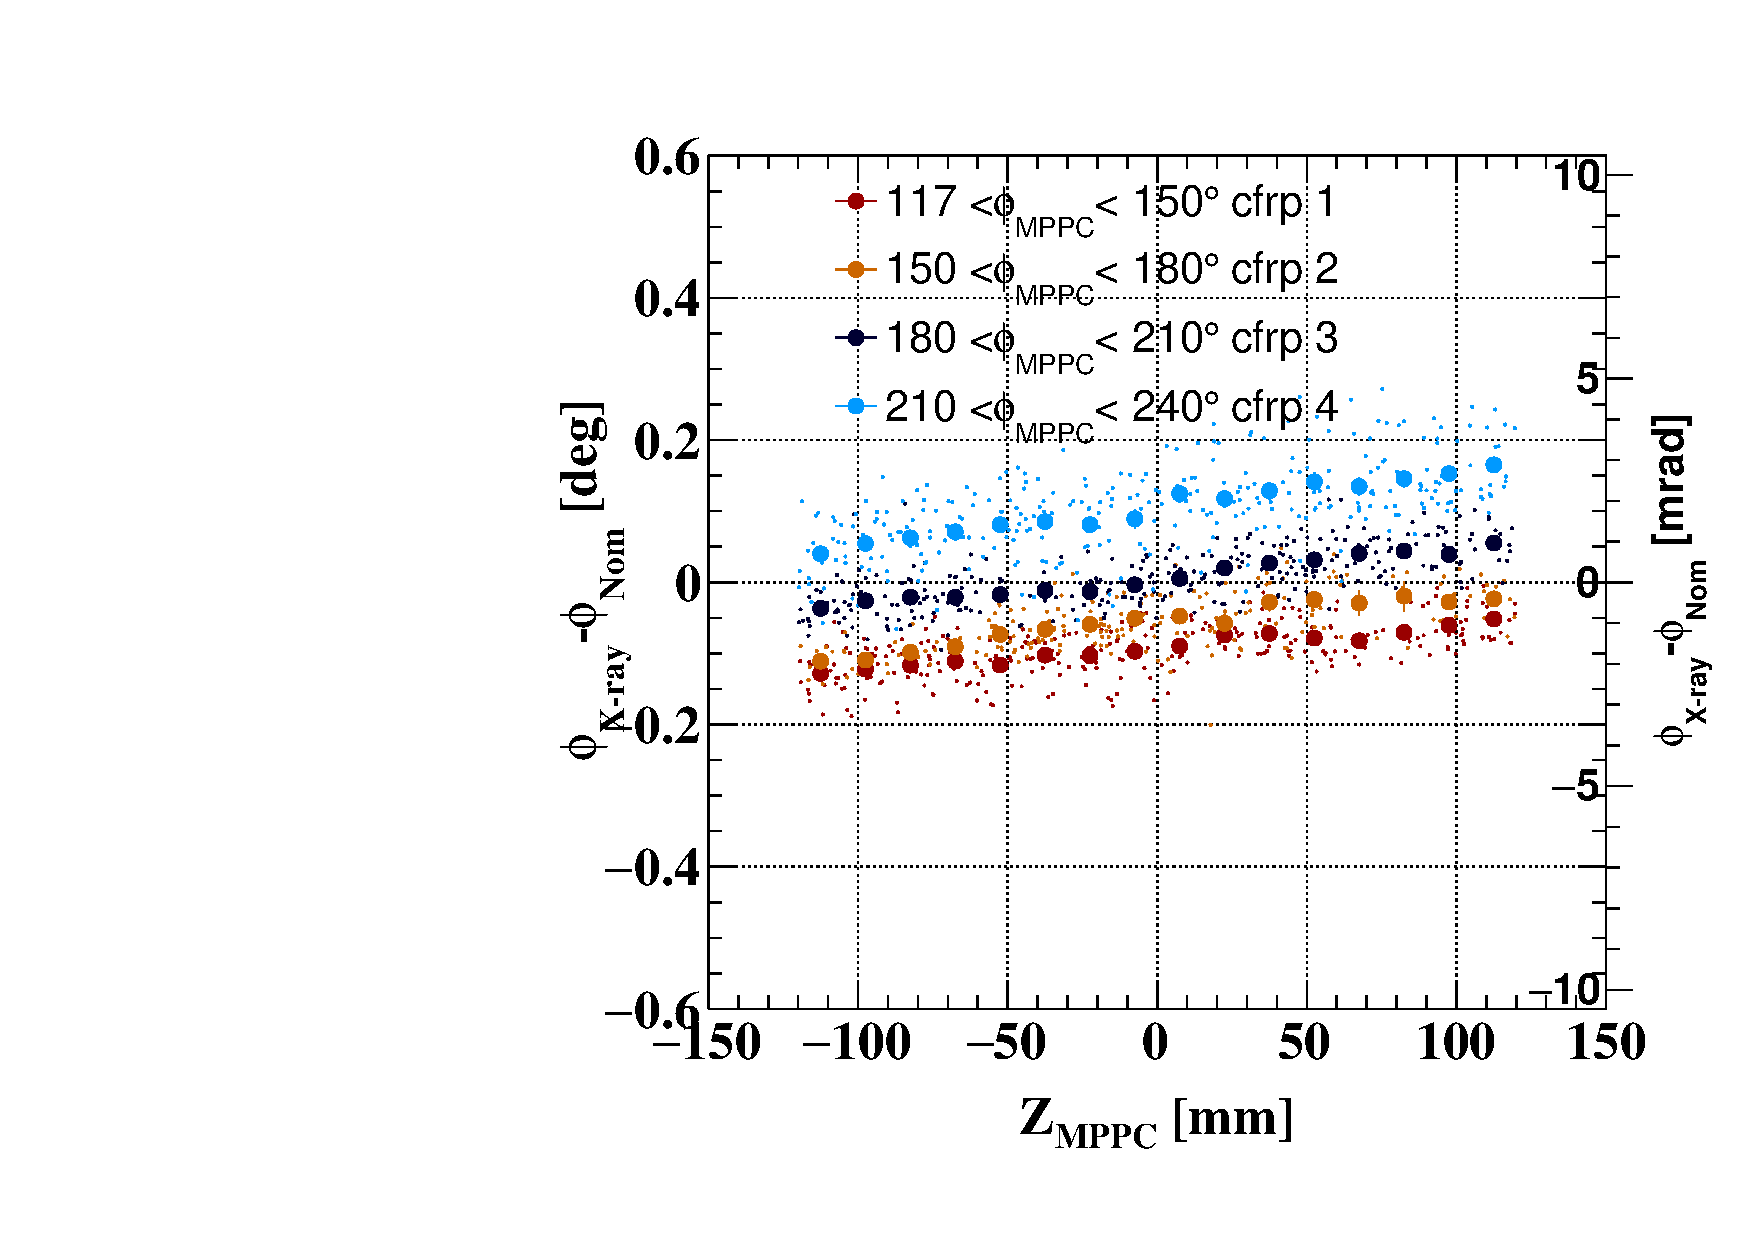
\includegraphics[width=4cm]{plots/dphi_boardrotation.pdf}\\
\caption{[add cfrp boundary]
Difference between the X-ray measured and nominal MPPC positions
overlayed with the profile histogram (scatter plots).
US and DS PCB half-strips and cfrp plates are shown separately.
Both Z and $\phi$ measurements have global offsets with respect to the 
nominal which are corrected in the plots.
}
\label{fig:rotation1}
\end{figure}

\begin{figure}
\begin{center}
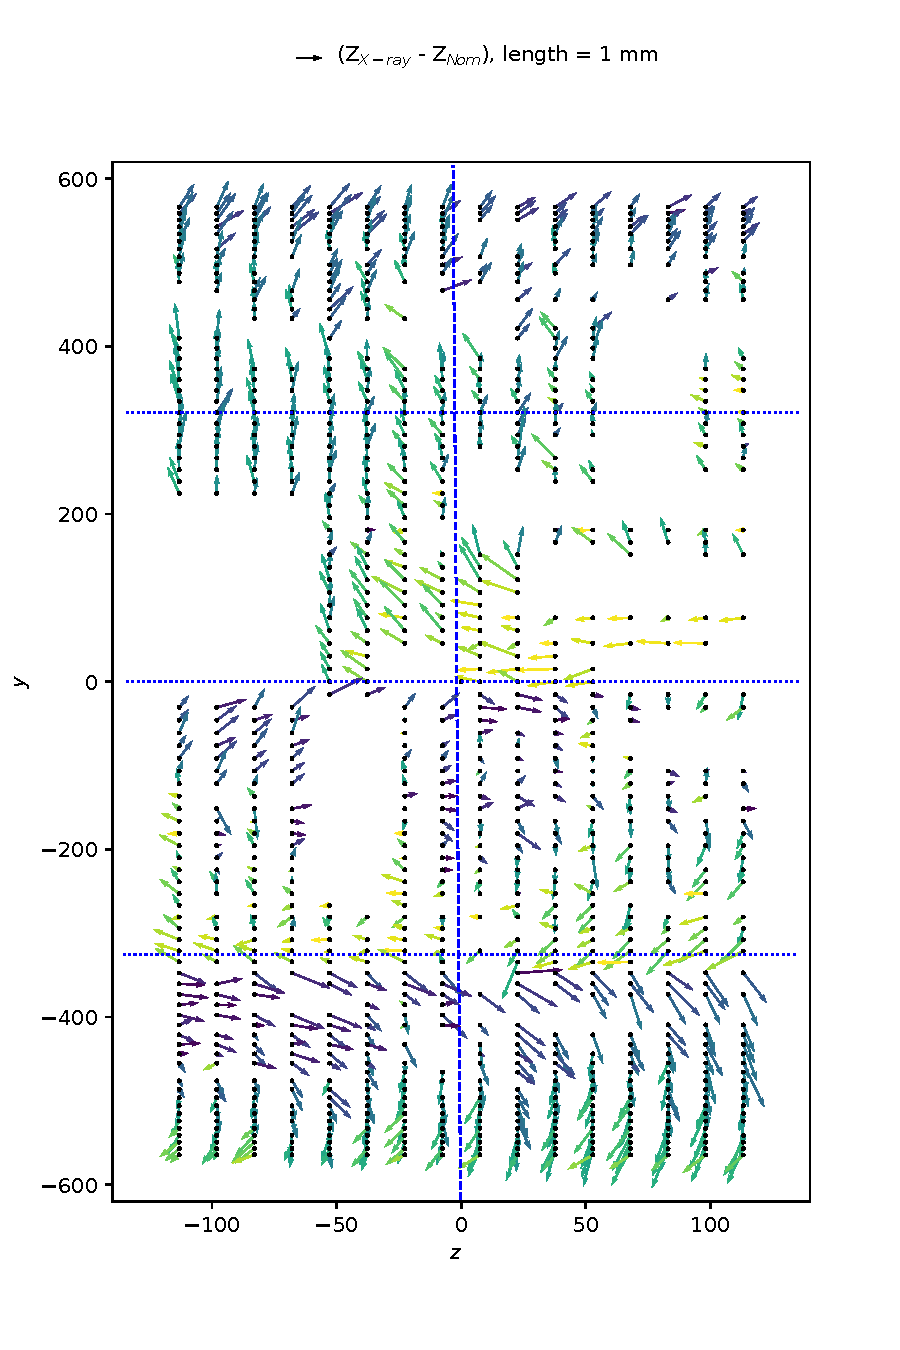
\includegraphics[width=6cm]{plots/dzdy2017_rx_test.pdf}
\caption{Arrow plot showing rotation of the MPPCs with respect to nominal
positions in the YZ plane; dotted horizontal lines show cfrp plate boundaries,
dashed vertical line at the center separates the PCB half-strips.
Both Z and $\phi$ measurements have global offsets with respect to the 
nominal which are corrected in the plots.
}
\label{fig:rotation2}
\end{center}
\end{figure}


The stability of the reconstructed position 
is verified by testing its dependence on 
the analysis procedure in two ways. 
First, the X-ray selection is performed using another independent criteria
and the fitting procedure is repeated.
Second, a different fitting function with higher-order Gaussian is
used. The pattern of X-ray event rates in each photodetector is fitted with
the function

\begin{equation} \label{eqn:supergauss}
    f(z)=b+s\cdot
Exp\left[-\left(\frac{z-\mu_{m}}{\sigma_{w}}\right)^{8}\right],
\end{equation}

where $b,s$ are the signal and background event rates. The 
flat-top of the function is centered at $\mu_m$,
and $\sigma_w$ determines the size  of
flat-top as well as the gaussian width of fall-off
on both sides. 
The results show new reconstructed positions consistent with the initial
calculation with mean 0.07~mm (0.2 mrad) and standard deviation
0.3~mm (0.45 mrad).


\section{Ancillary Measurements}
The entrance face of the LXe calorimeter consists of 4092 MPPCs
arranged in a grid structure containing 93 rows in the $\phi$ direction.  
A row consists of 44 MPPCs placed along $Z$ direction, divided equally in two
PCB\footnote{Printed Circuit Board} strips on the upstream and
downstream side of the calorimeter \cite{megdesign}.  The PCB strips
are mounted with spacer materials on four CFRP\footnote{Carbon Fiber
Reinforced Polymer} plates, each containing 23-24 strips and attached
to the inner face of the cryostat at different $\phi$ locations.  The
in-situ position and alignment of the MPPCs and its installation
assembly is verified in the following sections.

\subsection{ Spacing in Z and $\phi$}
The photodetectors are manufactured and assembled in lattice formation
to high precision, which can be used for validation of the X-ray
scanning technique and calculate its resolution.  A change in the
spacing can also reveal the effect of thermal cooling as well as
installation errors.  The spacing between individual MPPC pairs as
well as mean spacing between adjacent MPPC is calculated per PCB strip
(row-wise) along Z and per cfrp plate (column-wise) along \phis. 

Table \ref{tab:oddeven} shows spacing between individual MPPC pairs separated
into two groups which include alternate pairs along columns for Z measurement,
and rows for $\phi$ measurement.  Nominally we expect the spacing to be equal in
the two groups; the data shows the spacing in Z coordinate differs by 0.88~mm
and 0.74~mrad in the $\phi$ coordinate.  The average spacing over the scanned
region (shown in table \ref{tab:avgspacing}), however, is consistent with
expectation after accounting for thermal cooling.  
This implies a systematic shift or miscalculated position 
of one set of every other MPPC by 0.22~mm (0.18 mrad), and the oppposite 
shift for the complementary set, such there is not net displacement over the entire
row or column. 


The source of this discrepancy is not known.
Two possible causes were investigasted that could introduce observed 
systematic shifts in reconstructed MPPC positions with the periodicty of 
$\sim$30 mm, or two MPPC widths: X-ray corrections and trigger bias.
Although inaccurate corrections to the X-ray position can introduce the magnitude of 
displacement in MPPC position observed the periodicity of the corrections
does not match that of the observed effect; Z corrections have a period of 
100~mm while $\phi$ corrections are monotonic.
Similarly, studies of the effect of trigger configuration on the reconstructed position 
were not able to replicate this effect. 


As the scale of the systematic shift is small compared to the overall
X-ray measurement uncertainty as well as the precision goals of the
MEG experiment, it is expected to have minimal effect on the photon
position resolution.  We estimate this effect on photon reconstrution
using MC simulation.  A photon interaction is simulated at
normal distance equivalent to one radiation length
($\lambda_{LXe}\approx$ 2.75 cm) over a two dimensional surface
consisting of (20 $\times$ 20) photodetector array.  The dimensions and
spacing of the photodetectors are identical to the MPPC 
in the LXe calorimeter.  The isotropic distribution of photons generated as a
result is recorded by the photodetector array. The signal in each
photodetector is proportional to the solid angle subtended to the
interaction point, and detection efficiency determined by the photon
incident angle, measured in standalone tests.  
Each event is simulated with an interaction point
chosen randomly in a 30$\times$30~mm$^2$ region equivalent to two MPPC
widths, and reconstructed twice, with nominal and systematically
shifted photodetector positions by 0.22~mm.  The photon position is
reconstructed using weighted mean of the signal recorded in the
photodetectors.
The results show no mean displacement, while the photo 
position resolution is degraded by 0.08~mm in the 
measurement plane.

The mean distance between adjacent MPPCs is calculated using only the
measurements at the end of the row or column.  The precision of the
measurement is improved as a result compared to the pair-wise spacing
by  one (two) order of magnitude in Z ($\phi$).  In the Z coordinate,
the mean distance is calculated for each PCB strip as well as for the
half-strips (US and DS) connected at the center.  Similarly in the
$\phi$ coordinate, the mean distance is calculated within individual
cfrp plates and overall.  The mean and standard deviation of the
calculated mean distance in Z and $\phi$  show a regular grid
structure with no deformation in the scanned region (table
\ref{tab:avgspacing}).

The effect of thermal cooling is seen in Z with the mean distance
15.08~mm  or 30~\micron contraction between adjacent MPPCs. The mean
distance in $\phi$ is dependent on the X-coordinate of the
semi-cylindrical LXe calorimeter whose center is nominally aligned
with the center of the X-ray scanning device.  During the X-ray survey
the calorimeter was off-center, shifted towards the X-ray device by
3.85~mm increasing the mean angular spacing seen in the data.  The
following sections detail the qualitative use of X-ray data to measure
thermal contraction and 3D MPPC location.

\begin{table}
\begin{tabular}{ccccc}
 & $Z_{n} - Z_{n-1}$ &Std. Dev.& $\phi_{n} - \phi_{n-1}$ & Std. Dev. \\
 & [mm] &[mm]& [mrad]& [mrad]\\
\hline
Odd  $n$ & 15.10 & 0.25 & 24.12 & 0.54 \\ 
Even $n$ & 15.06 & 0.26 & 23.38 & 0.70 \\ 
%Nominal  & 15.1  &      & 23.55 & \\
\end{tabular}
\caption{Mean Z and $\phi$ spacing calculated for Odd-Even and Even-Odd
combination  of adjacent MPPCs.}
\label{tab:oddeven}
\end{table}
%Odd  $n$ & 15.69 & 0.49 & 24.12 & 0.54 \\ 
%Even $n$ & 14.57 & 0.57 & 23.38 & 0.70 \\ 

\begin{table}
\begin{tabular}{clc}
   & Z [mm] &Std. Dev. [mm] \\
\hline
US     & 15.091(32)& 0.127  \\
DS     & 15.101(49)& 0.164  \\
All    & 15.081(8) & 0.061  \\
Nominal& 15.1      &
\end{tabular}

\begin{tabular}{clc}
   & $\phi$ [mrad] &Std. Dev. [mrad] \\
\hline
cfrp 1     & 23.733(13)& 0.032  \\
cfrp 2     & 23.716(15)& 0.055  \\
cfrp 3     & 23.689(12)& 0.035  \\
cfrp 4     & 23.727(11)& 0.037  \\
All        & 23.725(2) & 0.008  \\
Nominal    & 23.55 &     
\end{tabular}
\label{tab:avgspacing}
\caption{Mean distance between adjacent MPPC calculated over the entire row (Z) or 
column ($\phi$). Upstream (US) and downstream (DS) parts of each PCB strip, and
individual cfrp plates are calculated separately, and altogether.}
\end{table}

\subsection {R coordinate calculation and 
coefficient of thermal expansion}
The radial coordinate not directly measured in the X-ray scan is
calculated using information from the FARO scan of the photodetectors.
The FARO scan provides highly precise 3D coordinates
($\sigma_{|\vec{x}|}$ = 200 \micron) of a subset of photodetectors
(10\%) measured at room temperature. To determine the position of
every photodetector, these measurements are interpolated by fitting
the 3D surface formed by the photodetectors. The radial coordinate and
center are calculted first with a cylindrical fit function, followed
by z,$\phi$ coordinates fitted to a regularly spaced grid in z-$\phi$
plane allowing for small rotations in the plane.  Each cfrp plate is
fitted independently since the curvature varies slightly between
individual plates and the overall curvature of the calorimeter.  


The interpolated photodetector locations from FARO
and X-ray scans are fitted with degrees of freedom to account for
global translational motion, extrinsic rotation centered in the MEG
coordinate  system, and scale factor for thermal contraction. 
The FARO coordinate is transformed using the equation
\begin{align}
\vec{x}_{FARO}^{'} = (1-s)R(\alpha,\beta,\gamma)\vec{x}_{FARO} +
\vec{x}_{offset},  
\end{align}
where $s$ is the scale of thermal contraction, $R$ is the rotation
matrix  and $\vec{x}_{offset}$ is the linear offset. 
The fit parameter values are extracted by minimizing the following function
\begin {align}
\chi^2 = 
\sum\limits_{i}^{N_{MPPC}} \frac{(Z_{i}^{Xray}-Z_{i,FARO}^{'})^2}{\sigma_{Z_{i}}^2} 
+ 
\frac{(\phi_{i}^{Xray}-\phi_{i,FARO}^{'})^2}{\sigma_{\phi_i}^2},
\end{align}
where $\sigma_{Z_i}$ and $\sigma_{\phi_i}$ include the resolution
of X-ray and FARO measurements
added in quadrature: 
$\sigma^{FARO}$ = 0.14~mm (0.25~mrad), 
$\sigma^{Xray}$ = 0.40~mm (0.56~mrad),
calculated from adjacent MPPC spacing described above.


The radial values from the FARO measurement are transformed using
fitted parameters to calculate radial coordinate of each
photodetector.  The uncertainty is calculated using linear error
propagation and corresponds to change in the main result due to one
standard deviation variation in the parameters taking correlations
into account.  The results in table \ref{tab:radius} shown mean radius
648.7 and 644.9~mm,and mean error 0.16 and 0.27~mm respectively in the
two scans(figure~\ref{fig:radiuscalculation}).  The radial coordinate
change of 3.8~mm between the two scans is consistent with the shift of
equal magnitude (3.85$\pm$0.1~mm) in the X-coordinate of the LXe
calorimeter in the same period.  A $\phi$ dependent change in the
radial coordinate is seen in 2018 data compared to the previous year's
data due to the calorimeter center offset with respect to the X-ray
device in 2018.



The thermal expansion coefficient is calculated as
\begin{align}
 s= \alpha_t \, \Delta T,
\end{align}
where s is the scale of thermal contraction, $\alpha_t$ is coefficient
of thermal expansion and $\Delta T$ is the change in temperature. 
Using $\Delta T$ ( = 123$\pm$10 K) 
between FARO survey performed at room temperature
(293 K) and X-ray survey performed at LXe temperature (170 K)
the thermal coefficient is calculated in the
two X-ray surveys (table \ref{tab:thermalcoefficient}).
\begin{table}[h]
\begin{tabular}{ccc}
Scan Period & $s$ & $\alpha_t \,\, [\mathrm{ppm K}^{-1}]$\\
\hline
2017 & 0.0015(1) & 11.7$\pm$1.9 \\
2018 & 0.0017(4) & 13.1$\pm$3.5 
\end{tabular}
\caption{Fitted scaling parameter ($s$) and the calculated thermal 
expansion coefficient.}
\label{tab:thermalcoefficient}
\end{table}
The theoretical value of $\alpha_t$ for the
detectaor material is 16$\pm$1 ppmK$^{-1}$.

The photodetector positions measured from the two X-ray surveys are
compared using the same fitting procedure to verify the stability 
of the photodetector ensemble.
The motion between the two
must be understood relative to the motion of the LXe calorimeter
position which has also moved between the two surveys.  Multiple
positions on the external surface of the calorimeter were optically
surveyed before each X-ray survey to record its location.  
Overall the motion of the calorimeter is replicated well 
by the photodetectors (table \ref{tab:xray2017vs2018}),
characterized by small angular rotations, and 
large displacement along X-axis seen in both data. 

\begin{table}[h] 
\begin{tabular}{rrr} 
Fit Paramter & Optical Survey &
X-ray Survey \\ 
\hline 
dx [mm] & 3.85 (7)      & 3.83 (6) \\ 
dy [mm] & -1.2 (2)      & -0.7 (2) \\ 
dz [mm] & 0.1 (2)       & -0.9 (2) \\ 
rx [mrad] & -0.0 (1)    & -0.1 (1) \\ 
ry [mrad] & -0.2 (2)    & 0.2 (4)    \\ 
rz [mrad] & -0.9 (2)    &  -0.3 (3)  
%%lxe
%%  1  rx          -4.98974e-05   1.12590e-04   1.81586e-08  -5.11285e-04
%%   2  ry          -2.46074e-04   1.69744e-04   8.54602e-09   1.55717e-02
%%   3  rz          -8.69646e-04   1.75347e-04   8.56504e-09   2.63737e-03
%%   4  dx           3.85602e+00   7.18101e-02   3.55683e-08   1.44061e-03
%%   5  dy          -1.18210e+00   2.30683e-01   3.55680e-08   7.98124e-04
%%   6  dz           1.45227e-01   2.24210e-01   3.55680e-08   3.00940e-03
%%
%%xray
%%   1  rx          -9.03902e-05   1.03847e-04   2.07576e-07  -4.03030e-03
%%   2  ry           1.73869e-04   3.56954e-04   1.50140e-07   8.05430e-03
%%   3  rz          -3.49186e-04   3.02230e-04   1.19763e-07  -2.19844e-02
%%   4  dx           3.83337e+00   6.64374e-02   4.16831e-07   2.82117e-03
%%   5  dy          -6.77152e-01   2.39740e-01   3.01004e-07   9.43571e-03
%%   6  dz          -9.02411e-01   1.90330e-01   2.49133e-07   5.52444e-03
\end{tabular}
\caption{Fit parameters denoting change in position of the calorimeter
(from optical survey) and the photodetector position (X-ray survey),
between the two data-taking periods, 2017 and 2018.}
\label{tab:xray2017vs2018} \end{table}



\begin{table}
\begin{tabular}{ccccc}
 & $R^{2017}$ & $\sigma_R^{2017}$ & $R^{2018}$  & $\sigma_R^{2018}$  \\
\hline
cfrp 1 &  649.3 & 0.16 & 645.4 & 0.27 \\
cfrp 2 &  648.9 & 0.17 & 644.3 & 0.27 \\
cfrp 3 &  648.7 & 0.17 & 644.5 & 0.27 \\
cfrp 4 &  648.1 & 0.15 & 645.3 & 0.27 \\
Average&  648.7 & 0.16 & 644.9 & 0.27 \\
\end{tabular}
\caption{Mean radius and error in mm in each cfrp plate for the two X-ray scans.}
\label{tab:radius}
\end{table}

\begin{figure}
\begin{center}
%\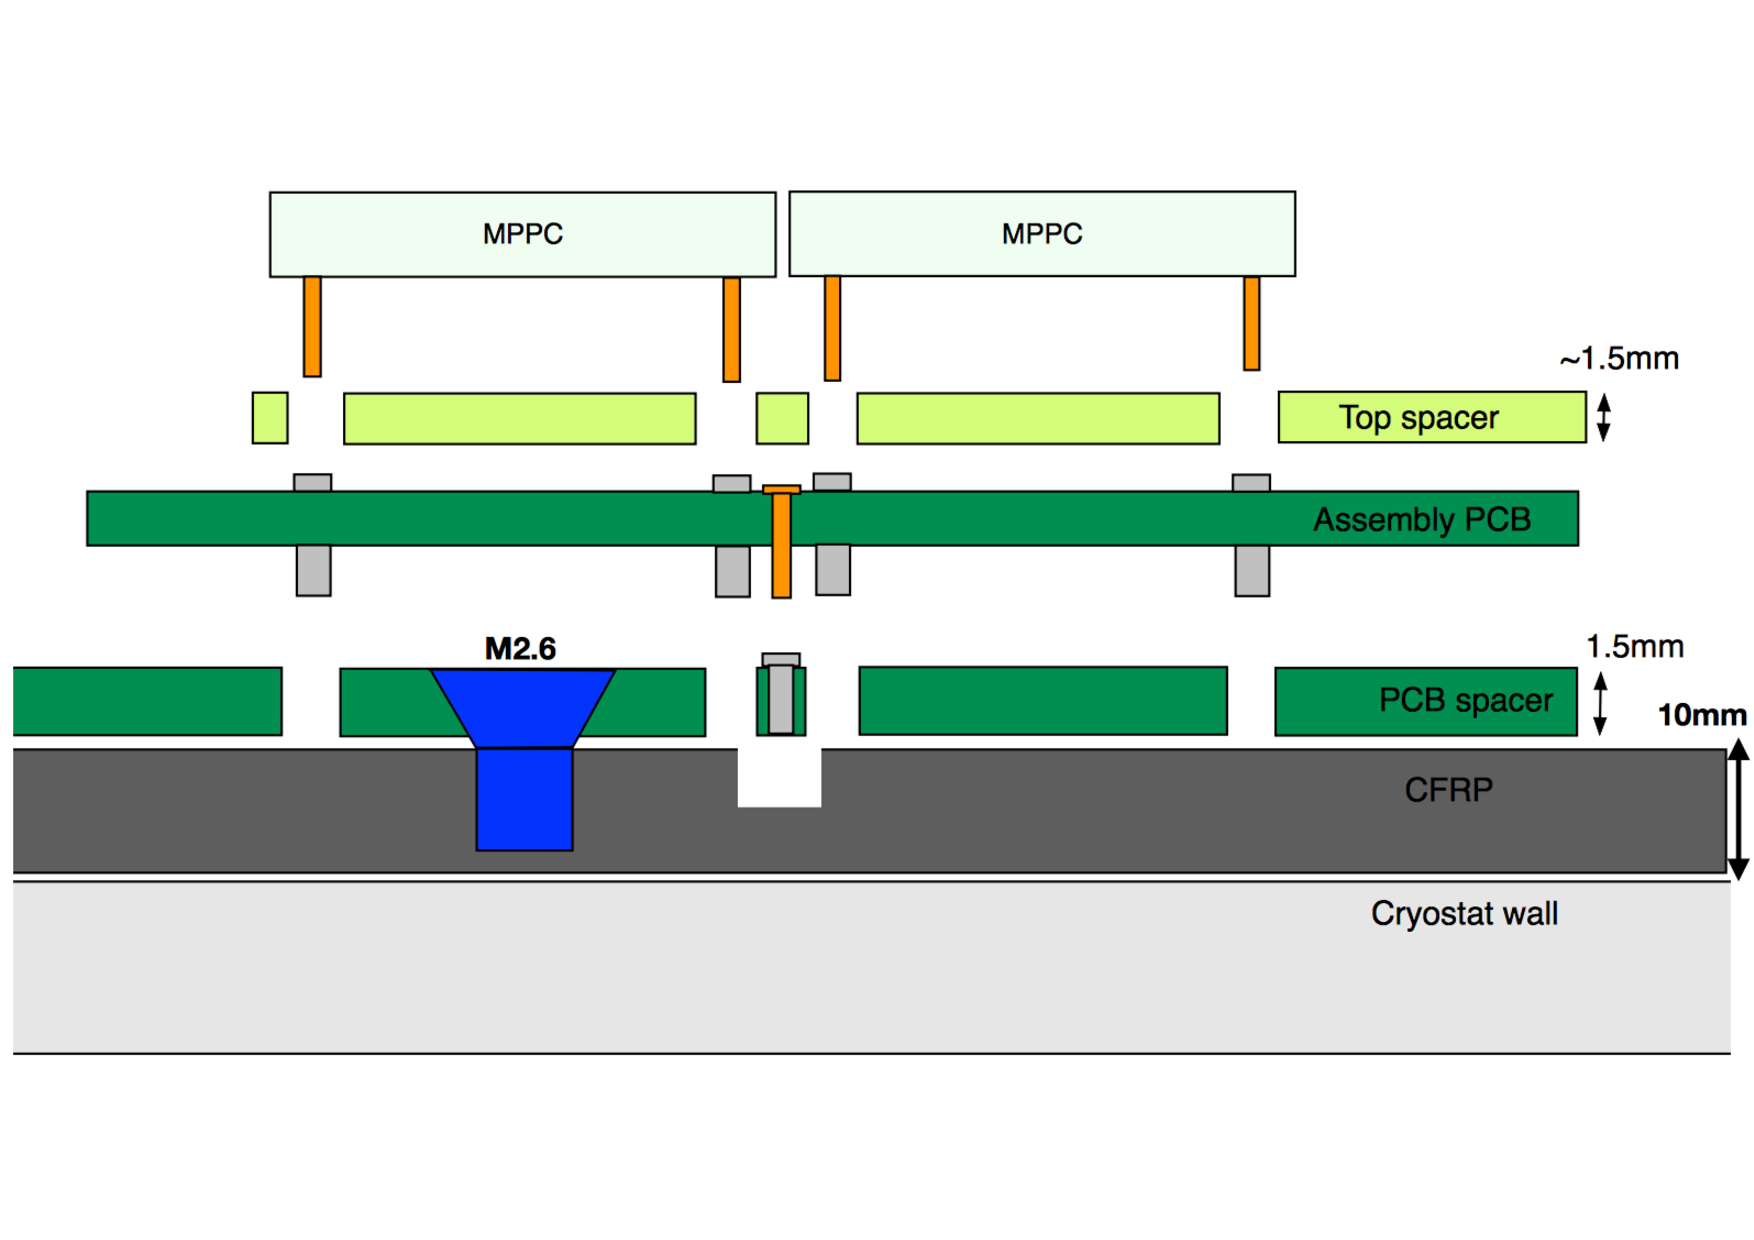
\includegraphics[width=4cm]{plots/MPPC_support.pdf}
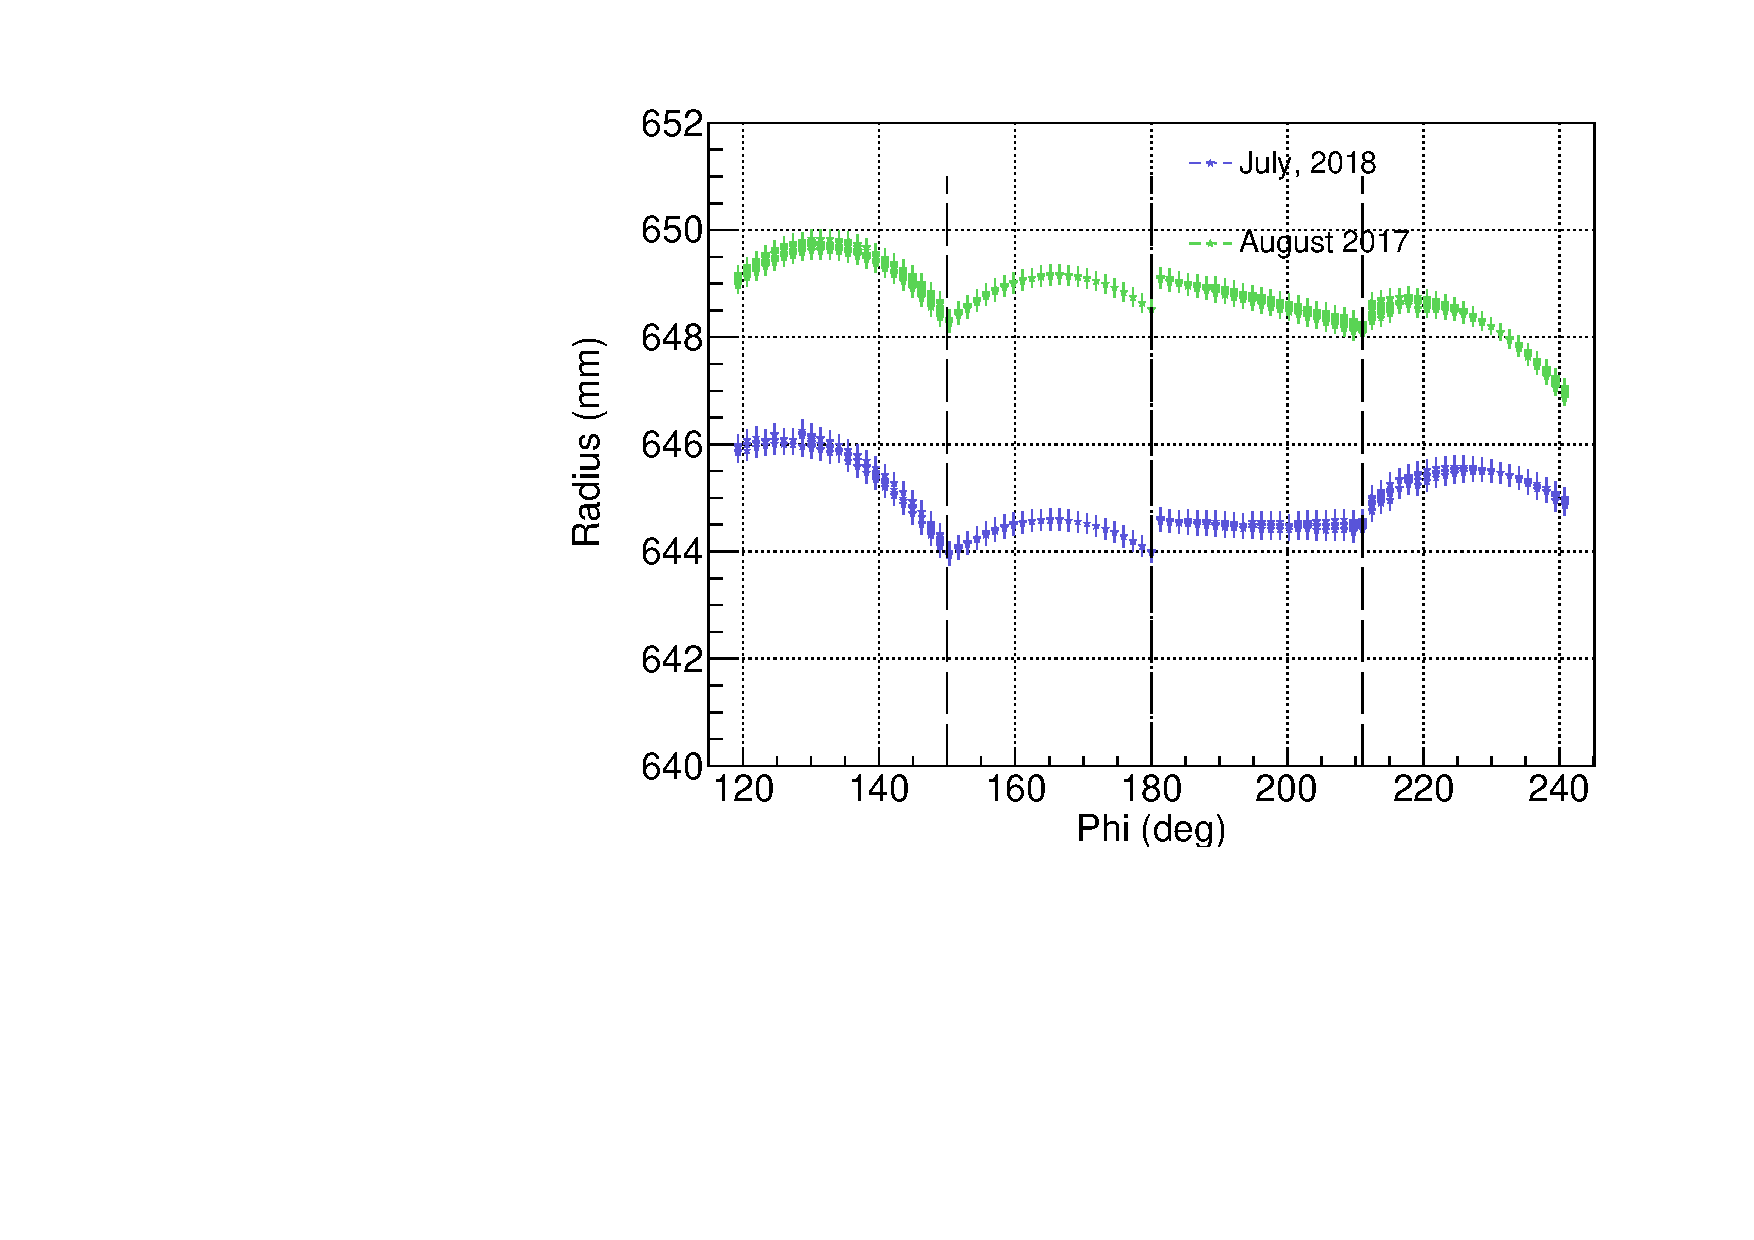
\includegraphics[width=4cm]{plots/2018/cRadius_1718}
\caption{ Radial coordinate of photodetectors with errors from 2017 and 2018
X-ray scans.  Black dashed lines indicate the edges of the CFRP plate.}
\label{fig:radiuscalculation} 
\end{center}
\end{figure}


\subsection { X-ray interaction rate -- 2017 vs 2018}  
The efficacy of spacer materials between MPPC, PCB strip and CFRP
plate is tested by examining the X-ray event rate as a function of
MPPC position. The rate is inversely proportional to the length of LXe
traversed by the X-ray before interaction.  It provides crucial
information about the state of spacer materials responsible for
preventing LXe leak between inner cryostat wall and the photosensitive
surface, which directly impacts photo detection and reconstruction
efficiencies, and energy response.  A constant rate of triggered
events is expected from all scanned MPPCs with some variation
attributed to electronic readouts that are nominally configured in an
identical way.  The event rates show a $\phi$ dependent variation
indicating some deformation in CFRP plates 1 and 2.  A drop in the
rates by a factor 1/e suggests the scale of deformation
$\approx\,\lambda_{\mathrm{Xe}}$.  The $\phi$ dependent variation is
observed in both Z and $\phi$ scans in the MPPCs illuminated with
X-rays and is not seen in the background process
(Figure~\ref{fig:ratesvszphi}).  The second scan in 2018 replicates
the previous years data at a lower rate due to reduced activity of the
source by two half-lives.  
\begin{figure}[]
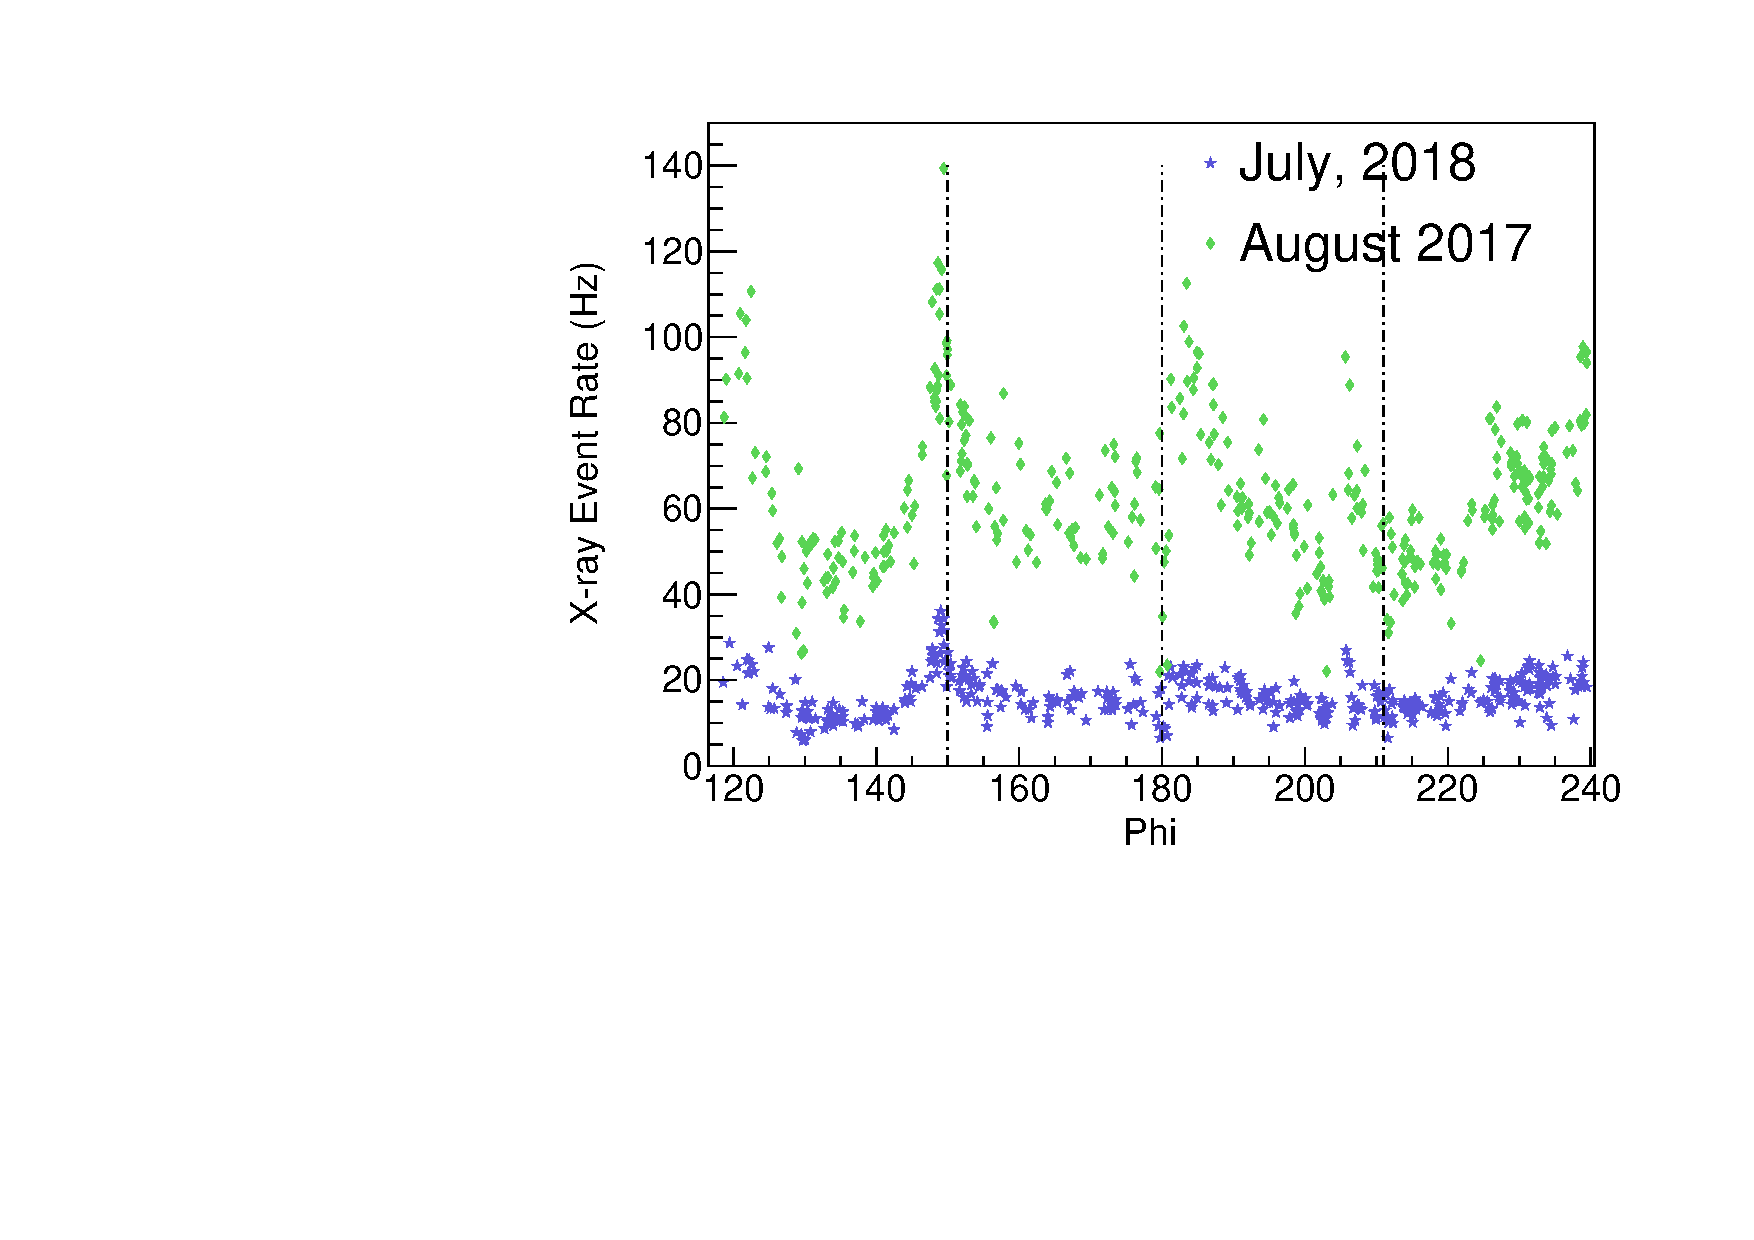
\includegraphics[width=4cm]{plots/2018/cEventRate_1718}
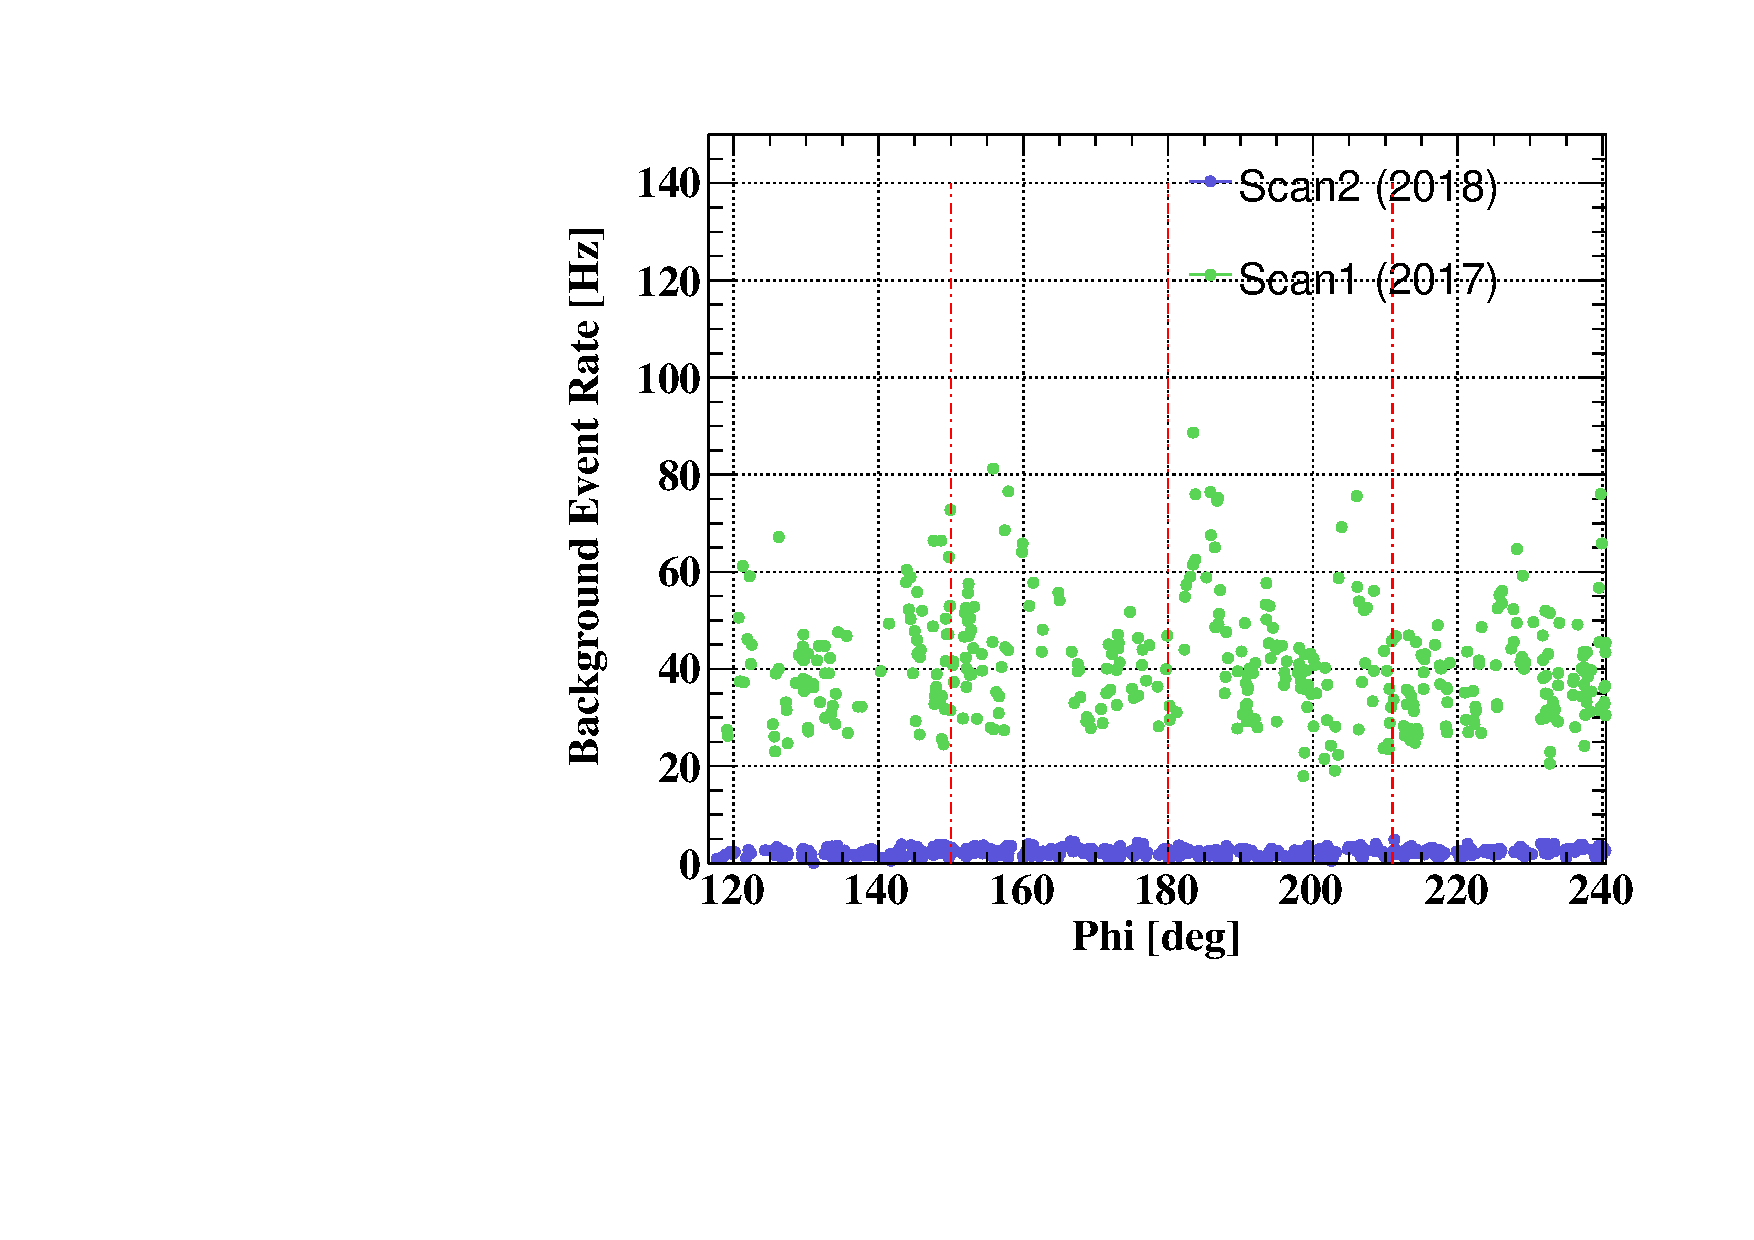
\includegraphics[width=4cm]{plots/2018/cBkgRate_1718} \caption{Signal
and background trigger rates observed in MPPC as a function of $\phi$.
Black lines indicate the edges of the CFRP plate.}
\label{fig:ratesvszphi} \end{figure}



\subsection{Charge Asymmetry} \label{sec:chargeasym}


An additional measurement of each photodetector's edge location was
determined by fitting charge asymmetries (Eqn. \ref{eqn:qasym}) between
adjacent photodetectors. This allows for a determination of
photodetector edges as defined by the midpoint between two detectors,
in which the X-ray induces charge measurements.

Event selection includes two classes of events; where the X-ray
induced charge is present in one of the channels, or shared by the two
adjacent channels.  The selection described in Sec.
\ref{sec:mppcposition} applied for single photodetector scan is used
with additional criteria to include events with X-ray interactions
between two photodetectors.  The requirement of minimal largest charge
may be satisfied either by a single illuminated channel, or by the sum of two adjacent channels.  Due to large variation in the gain
of individual photodetectors, the charge from each photodetector is
normalized to avoid skewing the asymmetry distribution. The mean
charge is calculated for each photodetector in the central scanning
region and normalized before applying selection.

The charge asymmetry for a given photodetector $i$
is calculated per event are as,  
\begin{equation} \label{eqn:qasym}
    A(Q)  = 
\frac{Q_{i}-Q_{i+1}}
     {Q_{i}+Q_{i+1}}, 
\end{equation}
where adjacent photodetector pairs ($i, i+1$) are chosen
along the direction of the coordinate scanned. The mean value
as a function of the coordinate is fitted to the 
following sigmoid function
\begin{equation}\label{eqn:asymfit}
f_{Asym}(z)=\;
C\,\left[\,Erfc(a(z-z_{0}))-1\,\right],
\end{equation} 
where $z_0$ is the offset in Z, and $C$ and $a$ are 
the scaling parameters of the function.

The center of the asymmetry distribution, $A(Q)=0$ in fig.
\ref{fig:asymplot}, consistutes the physical edge of the
photodetector.  Using both edges, the photodectector position and its
size is independently calculated, in each Z and \phis coordinate.  A
comparison between calculated photodetector position using X-ray event
rates and charge asymmetry (fig. \ref{fig:asymvsfit}) shows the two
measurements to be consistent.  The photodetector size calculated with
asymmetry (fig. \ref{fig:mppcsize}) is also in good agreement with the
average spacing of the photodetectors previously calculated (table
\ref{tab:avgspacing}).  Due to trigger configuration and the
particular scanning region used in the X-ray survey, photodetectors on
the boundary of trigger region are excluded from the calculaton,
limiting this measurement to 15\% of the scanned photodetectors.


\begin{figure}
\centering
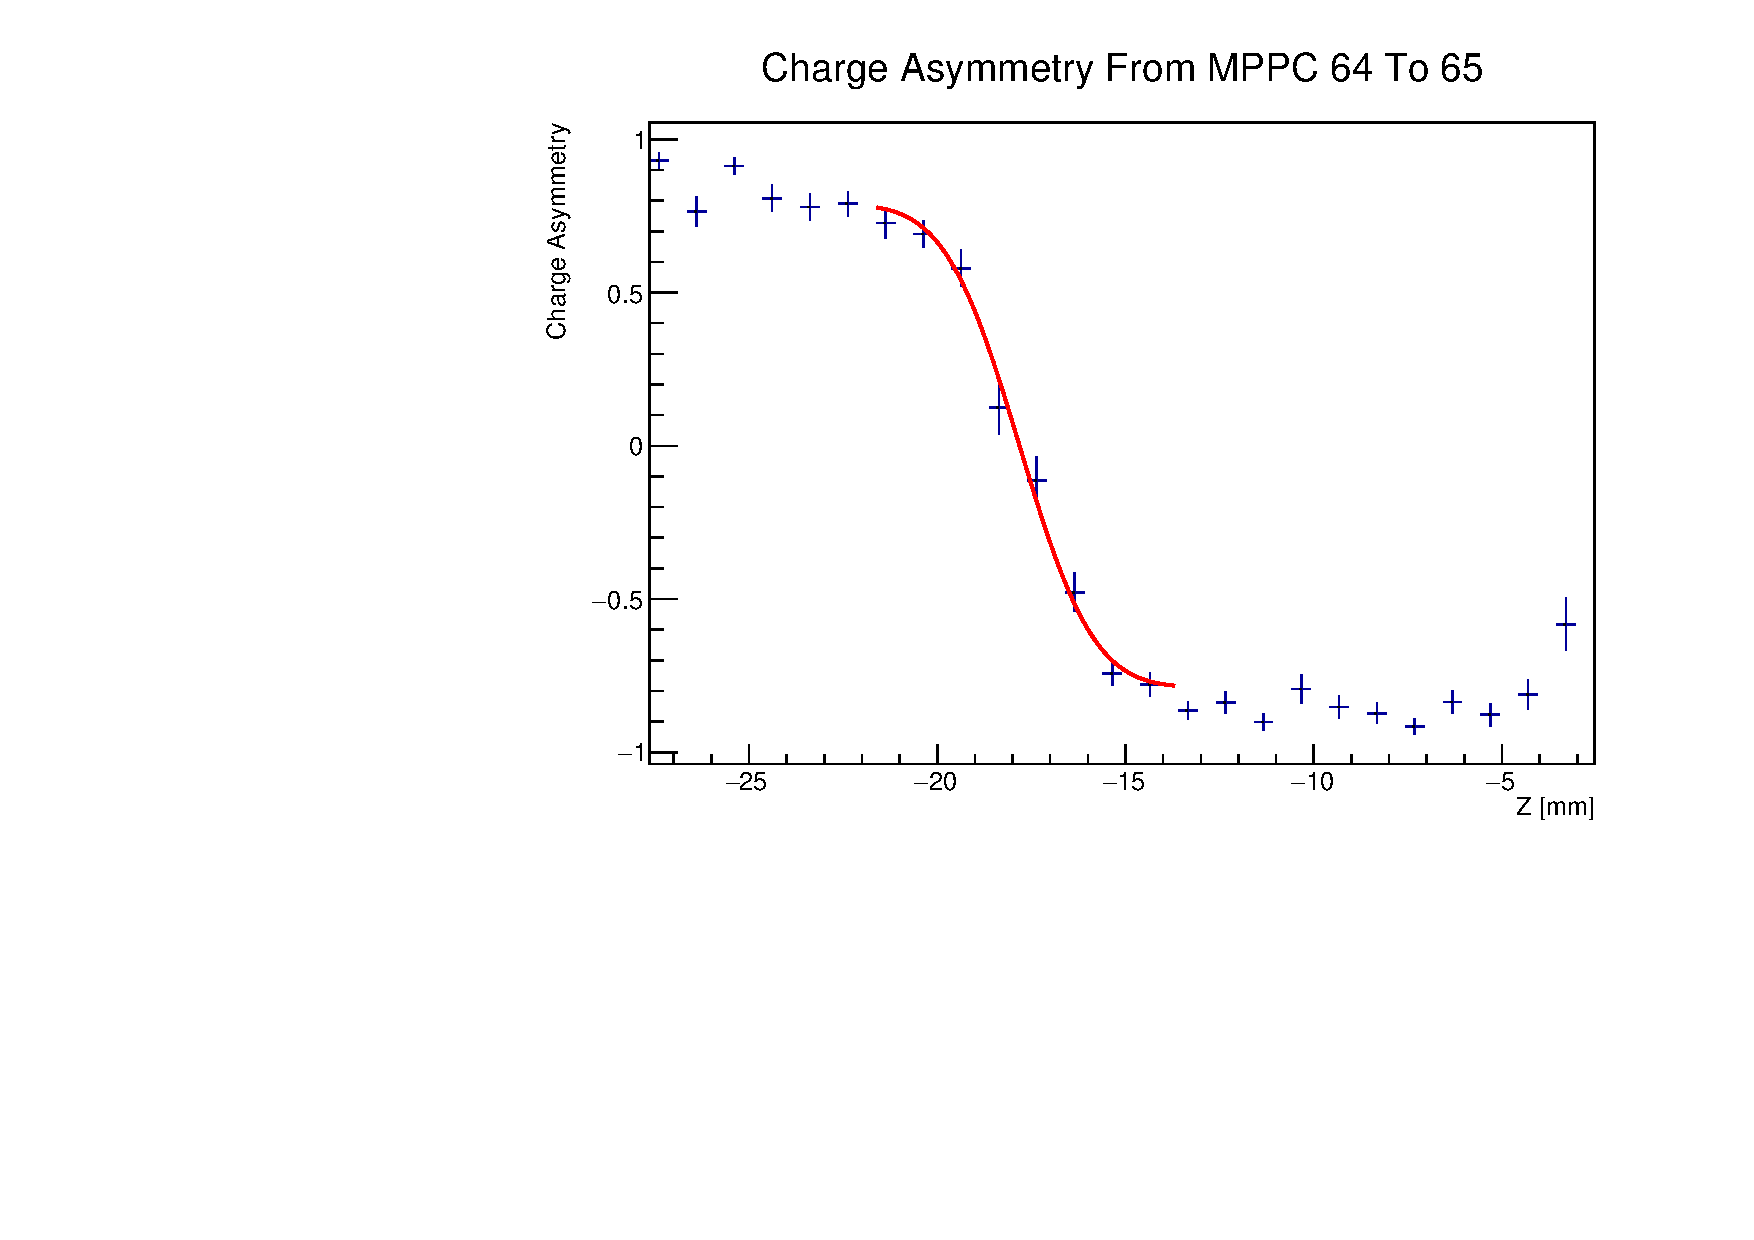
\includegraphics[width=4cm]{graphics/asym6465.pdf}
\caption{Mean charge asymmetry calculated as a function of z between 
two photodetectors.}
\label{fig:asymplot} 
\end{figure}

\begin{figure}
\centering
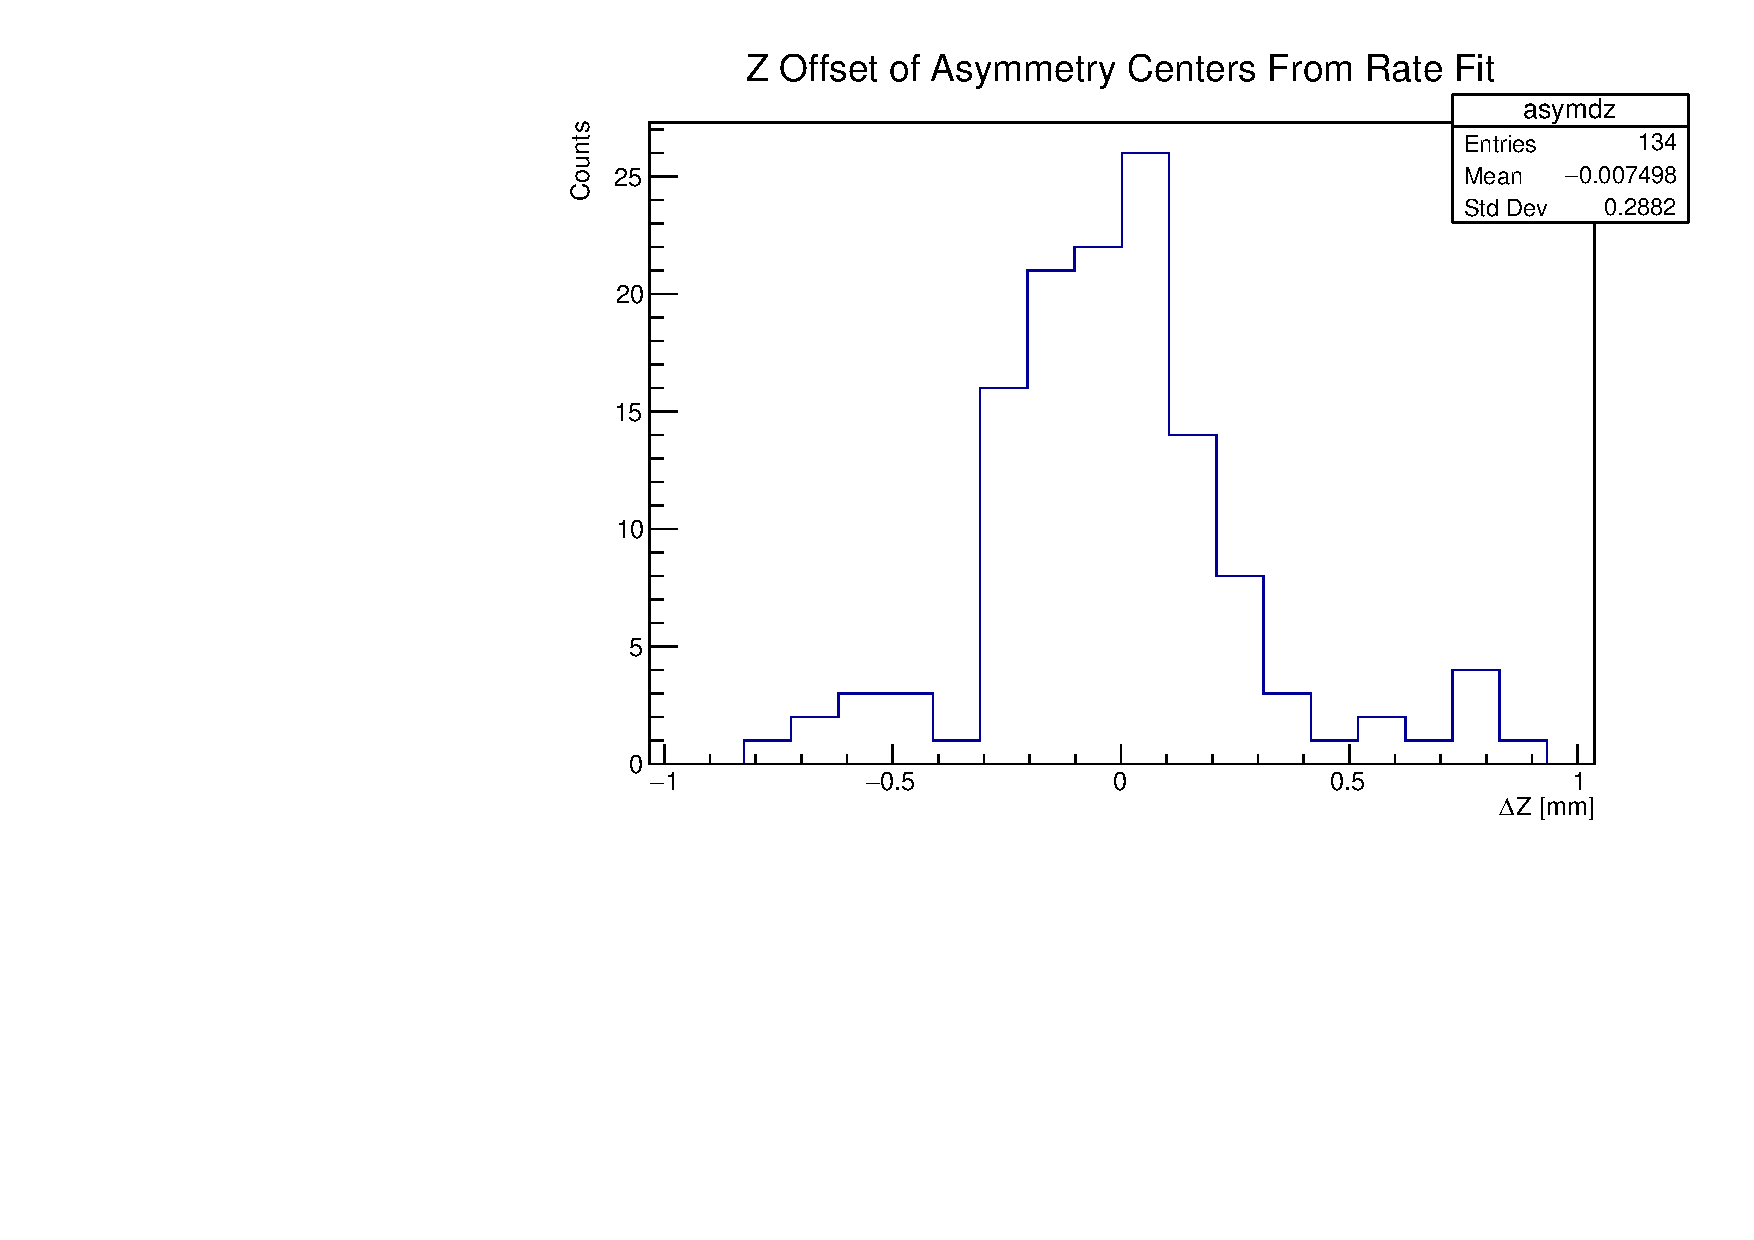
\includegraphics[width=4cm]{asymmetryplots/asymdz.pdf}
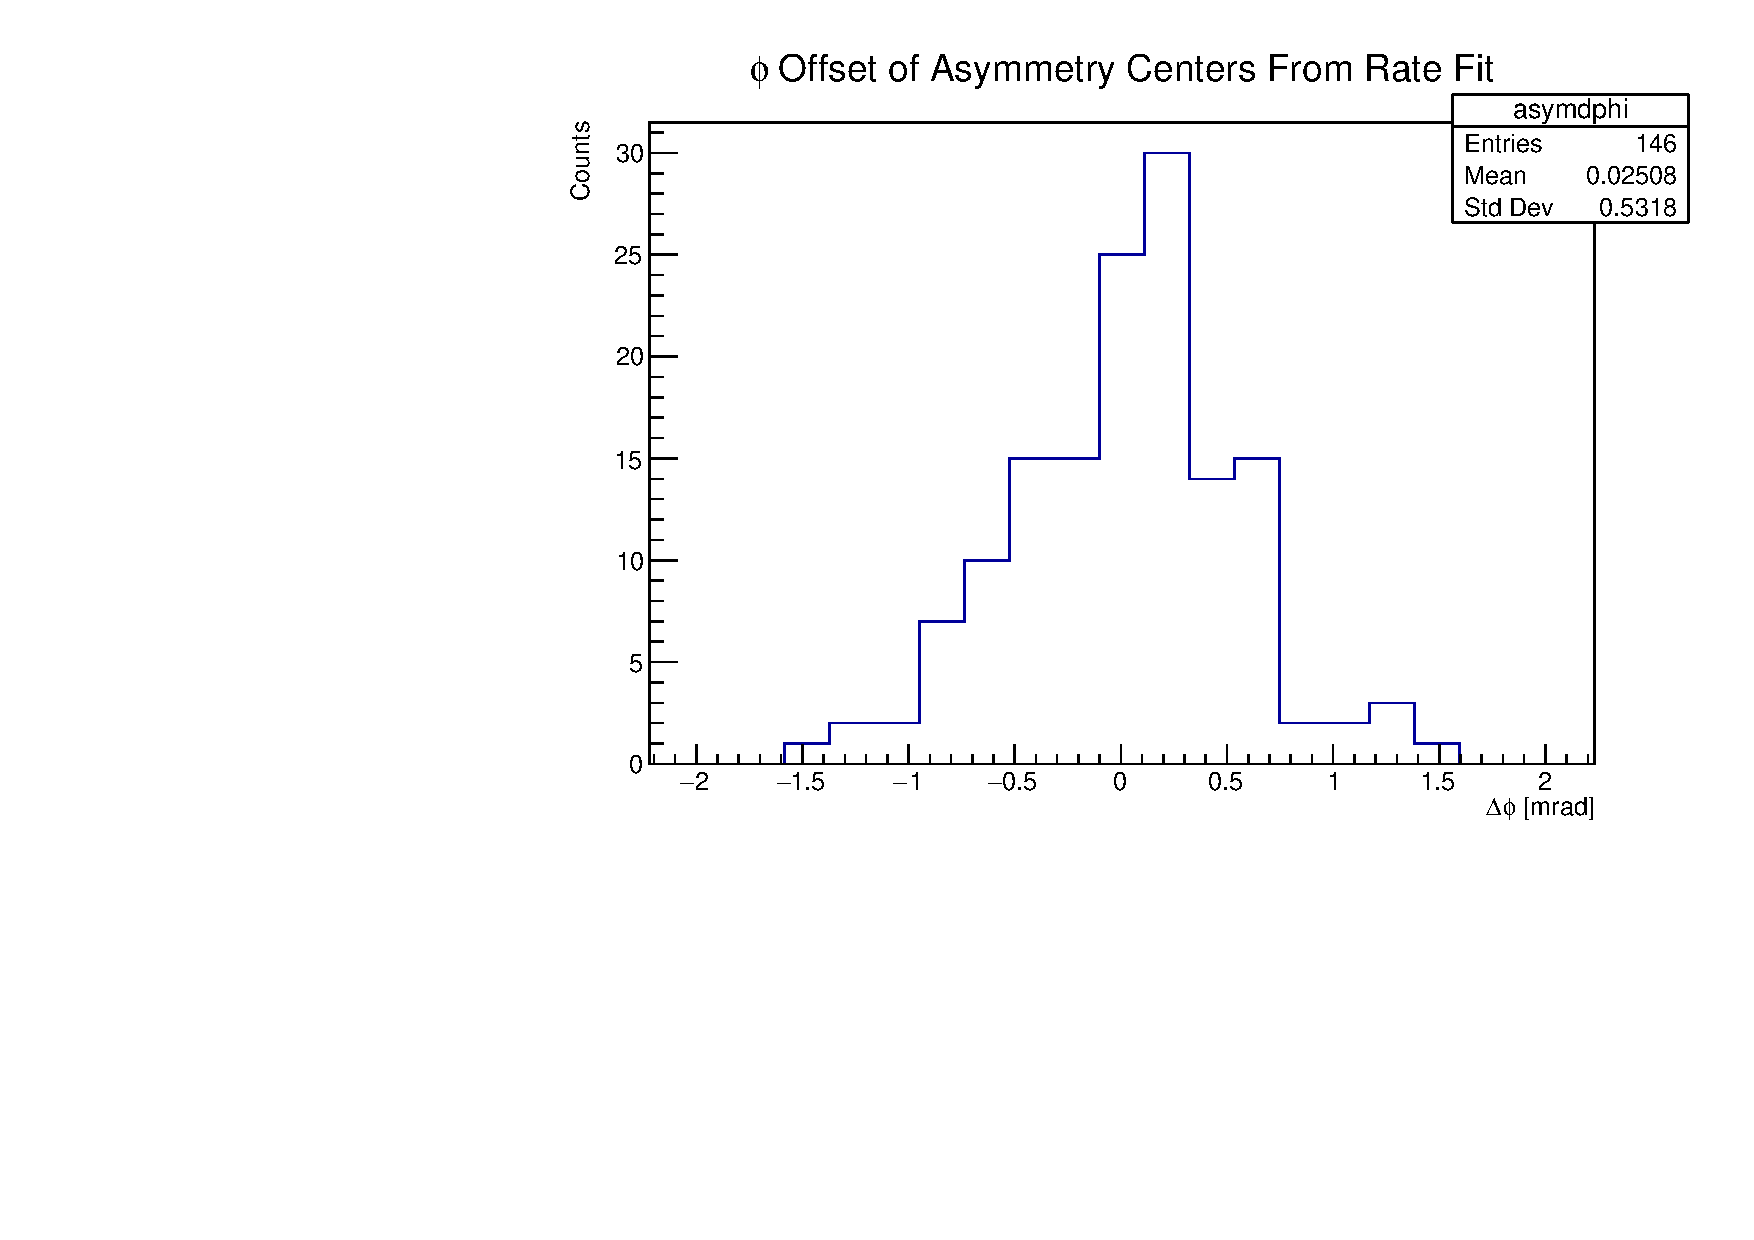
\includegraphics[width=4cm]{asymmetryplots/asymdphi.pdf}
\caption{Comparison between photodetector position calculated from
charge asymmetry and X-ray event rates.}
\label{fig:asymvsfit} 
\end{figure}



\begin{figure}
\centering
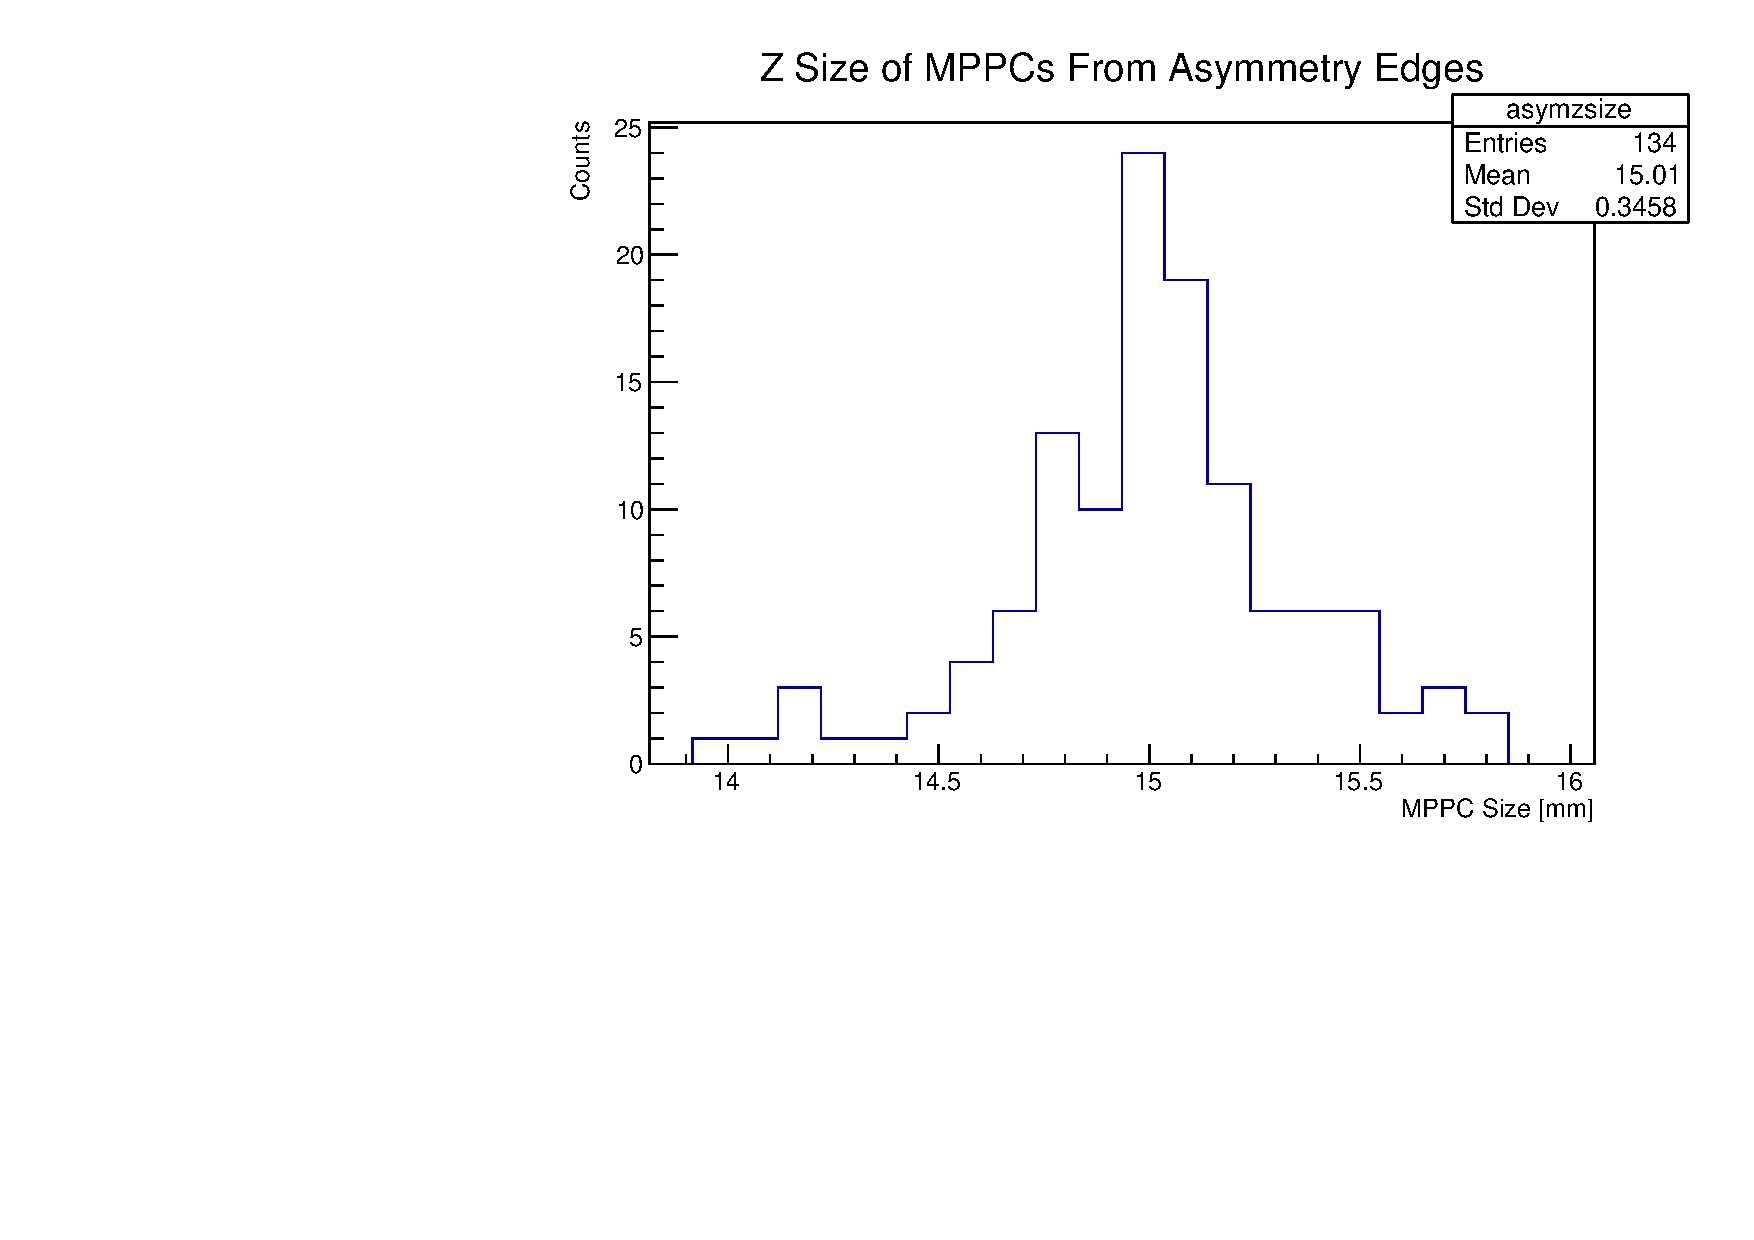
\includegraphics[width=4cm]{asymmetryplots/asymzsize.pdf}
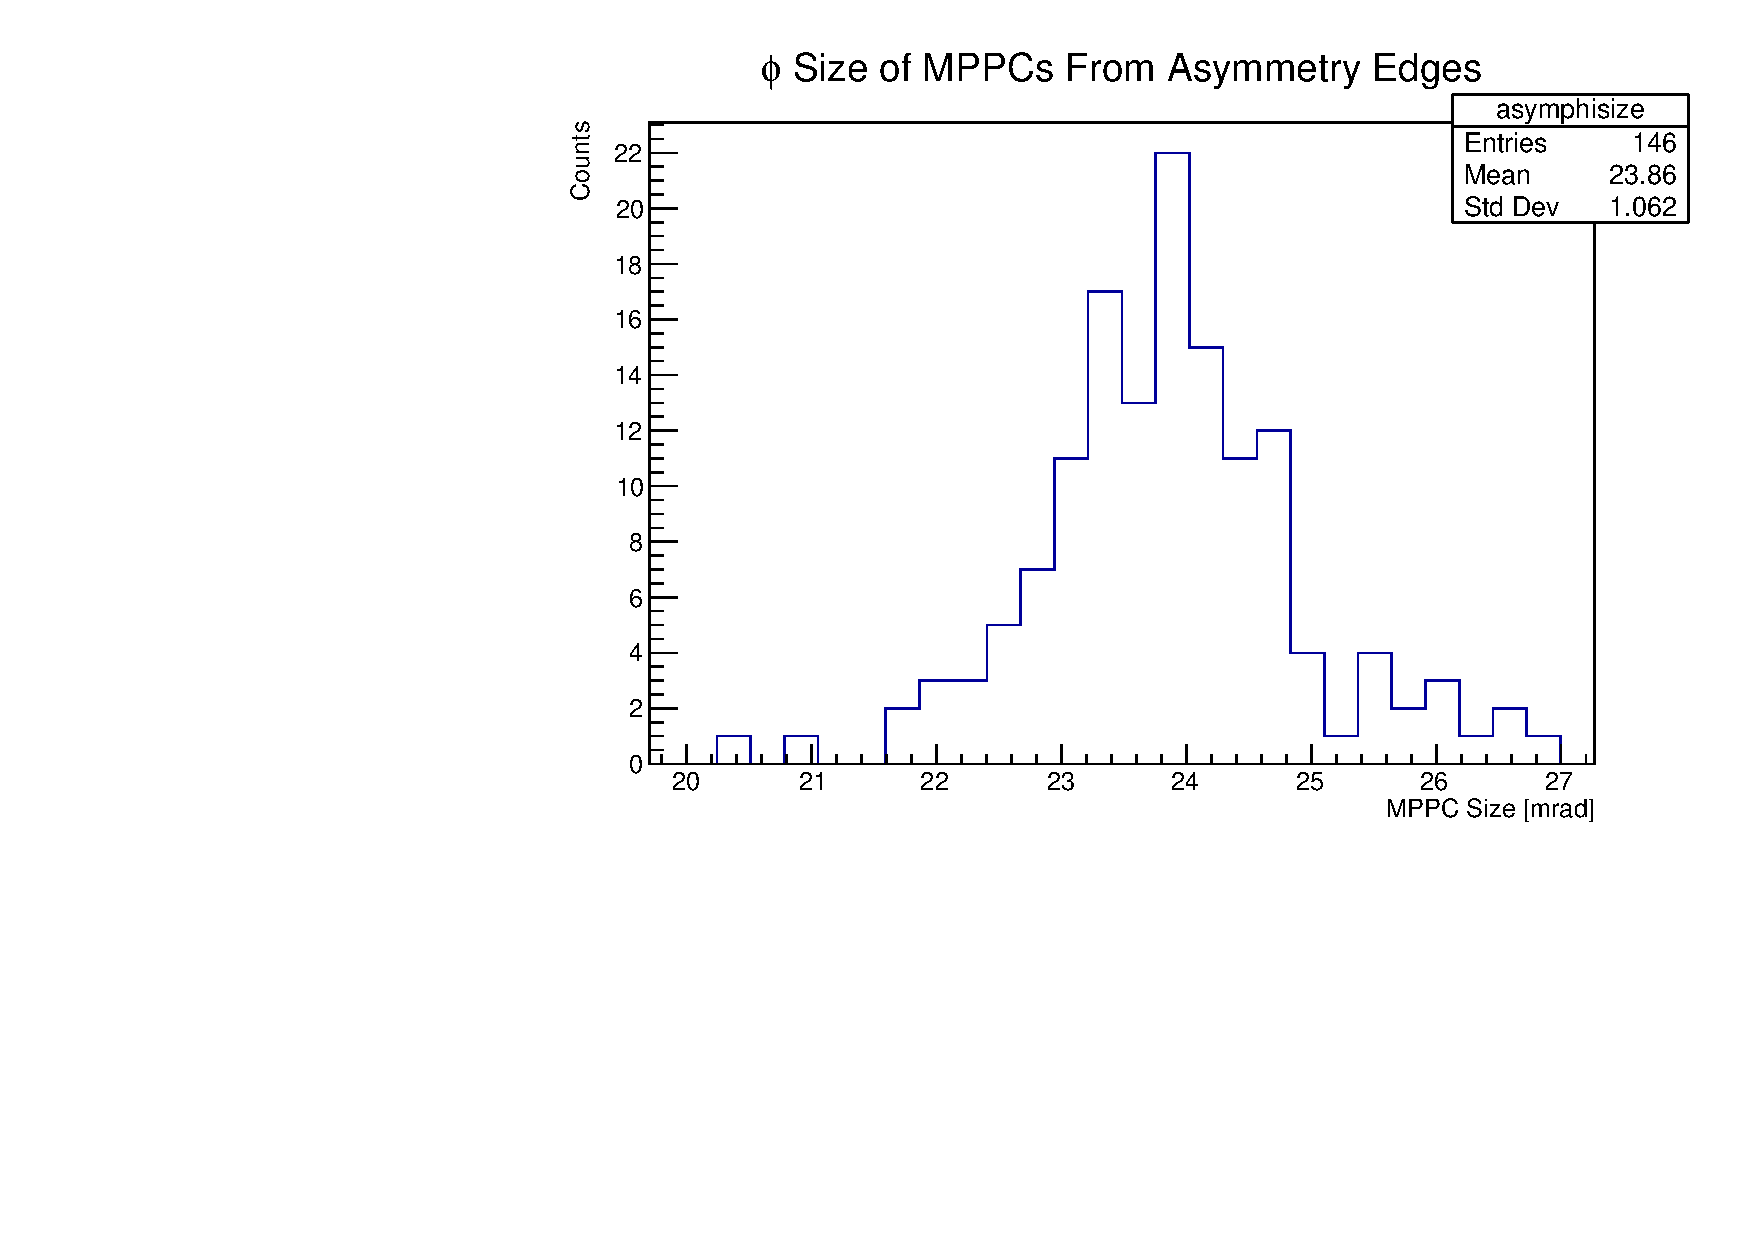
\includegraphics[width=4cm]{asymmetryplots/asymphisize.pdf}
\caption{Photodetector size in Z and phi measured using the edge of the
photodetector calculated with charge asymmetry.}
\label{fig:mppcsize} 
\end{figure}



%With these additional measurements, it is possible to produce a
%comparison to our prior findings on the photodetector spacing. For
%this purpose, we calculate all the possible offsets of detectors edges
%(per asymmetry fits) from their previously fitted central locations. 

%%%%%%%\begin{table}[H]
%%%%%%%    \centering
%%%%%%%    \begin{tabular}{c||c|c}
%%%%%%%        \bf Upper Edge & \bf \boldmath$\mu$ [mm] & \bf \boldmath$\sigma_{RMS}$ [mm] \\
%%%%%%%         \hline
%%%%%%%        Even, 1 of 4 & 7.954 & 0.500 \\
%%%%%%%        Even, 3 of 4 & 7.824 & 0.409 \\
%%%%%%%        Even, 1 of 2 & 7.82 & 0.438  \\
%%%%%%%        Odd, 2 of 4 & 7.713 & 0.396  \\
%%%%%%%        \hline
%%%%%%%        All Even & 7.862 & 0.451 \\
%%%%%%%        All Odd & 7.713 & 0.396
%%%%%%%    \end{tabular}
%%%%%%%    \caption{Measured Z Offsets of Upper Edges From Fit Centers}
%%%%%%%    \label{tab:upperedgeasymz}
%%%%%%%\end{table}
%%%%%%%
%%%%%%%\begin{table}[H]
%%%%%%%    \centering
%%%%%%%    \begin{tabular}{c||c|c}
%%%%%%%         \bf Lower Edge & \bf \boldmath$\mu$ [mm] & \bf \boldmath$\sigma_{RMS}$ [mm] \\
%%%%%%%         \hline
%%%%%%%         Odd, 2 of 4 & 7.363 & 0.385 \\
%%%%%%%         Odd, 4 of 4 & 7.771 & 0.413 \\
%%%%%%%         Odd, 2 of 2 & 7.816 & 0.410 \\
%%%%%%%         Even, 3 of 4 & 7.154 & 0.436 \\
%%%%%%%         \hline 
%%%%%%%         All Even & 7.154 & 0.436 \\
%%%%%%%         All Odd & 7.669 & 0.448
%%%%%%%    \end{tabular}
%%%%%%%    \caption{Measured Z Offsets of Lower Edges From Fit Centers}
%%%%%%%    \label{tab:loweredgeasymz}
%%%%%%%\end{table}
%%%%%%%
%%%%%%%\begin{table}[H]
%%%%%%%    \centering
%%%%%%%    \begin{tabular}{c||c|c}
%%%%%%%        \bf Upper Edge & \bf \boldmath$\mu$ [mrad] & \bf \boldmath$\sigma_{RMS}$ [mrad] \\
%%%%%%%         \hline
%%%%%%%        Even, 1 of 4 & 12.05 & 1.023 \\
%%%%%%%        Even, 3 of 4 & 12.56 & 0.7336 \\
%%%%%%%        Even, 1 of 2 & 12.28 & 0.357  \\
%%%%%%%        Odd, 2 of 4 & 12.23 & 1.125  \\
%%%%%%%        \hline
%%%%%%%        All Even & 12.32 & 0.884 \\
%%%%%%%        All Odd & 12.23 & 1.125
%%%%%%%    \end{tabular}
%%%%%%%    \caption{Measured $\phi$ Offsets of Upper Edges From Fit Centers}
%%%%%%%    \label{tab:upperedgeasymphi}
%%%%%%%\end{table}
%%%%%%%
%%%%%%%\begin{table}[H]
%%%%%%%    \centering
%%%%%%%    \begin{tabular}{c||c|c}
%%%%%%%         \bf Lower Edge & \bf \boldmath$\mu$ [mrad] & \bf \boldmath$\sigma_{RMS}$ [mrad]\\
%%%%%%%         \hline
%%%%%%%         Odd, 2 of 4 & 11.87 & 0.715 \\
%%%%%%%         Odd, 4 of 4 & 11.99 & 0.629 \\
%%%%%%%         Odd, 2 of 2 & 11.83 & 0.340 \\
%%%%%%%         Even, 3 of 4 & 11.42 & 0.717 \\
%%%%%%%         \hline
%%%%%%%         All Even & 11.42 & 0.717 \\
%%%%%%%         All Odd & 11.93 & 0.654
%%%%%%%    \end{tabular}
%%%%%%%    \caption{Measured $\phi$ Offsets of Lower Edges From Fit Centers}
%%%%%%%    \label{tab:loweredgeasymphi}
%%%%%%%\end{table}
%%%%%%%
%%%%%%%Included above is a separation based upon location of each measurement
%%%%%%%within the trigger region of a scan, and is listed as an index from 1
%%%%%%%to either 2 or 4, depending upon the number of detectors the beam
%%%%%%%traversed within a scan.



%%\subsection{Charge Asymmetry}
%%\noindent Definition \\
%%Selection of events \\
%%Charge (sharing) fraction between adjacent mppc \\
%%Gain equalization and fitting  \\
%%Comparison to earlier calculations of position and spacing. \\


\subsection{Quantum Efficiency$\times$Gain}
An uniform source of light provided by the collimated X-ray beam is
used to measure relative gain of the photodetectors.  The mean charge
response, proportional to the gain and quantum efficiency, is measured
with a good spatial precision in the X-ray survey.  Assuming the
quantum efficiencies are identical, the mean charge response is
analyzed to determine the stability and uniformity of photodetector
gain over the scanned region of the calorimeter.  It must be noted
that the charge measurement contains smaller but inseparable
contributions from after-pulse and cross-talk between neighboring
photodetectors, which are independent from the photodetector gain.
Additionally, only relative measurement of gain is possible as the
absolute photon yield in the X-ray interaction relies on other factors
such as presence of impurities in the liquid Xenon which were not
precisely known. 


The photodetectors are developed according to the experimental
requirements with large photosensitive area 12 $\times$ 12 mm$^2$,
comprised of four  smaller pixels 6 $\times$ 6 mm$^2$ connected in
series.  The photodetectors are placed in a ceramic case (15 mm) and
mounted on a PCB strip, each containing 22 photodetectors.  Two
identically produced strips aligned along $\hat{z}$ direction, and
rotated by 180\degree with respect to each other to allow for
electronics readout at each end, make up a single row (fig 
\ref{fig:mppc}).
The mean charge  is calculated over the 12 mm region centered at the
fitted photodetector location from previous analysis.  Due to long
tail in the charge distribution an iterative gaussian fit is used,
initially over the entire range and then restricted to the two sigma
region of the first fit.  The mean charge varies overall between the
scanned photodetectors by 50\%, and correlates reliably with the
production batch of the photodetectors (fig \ref{fig:mppccharge}). 

\begin{figure}
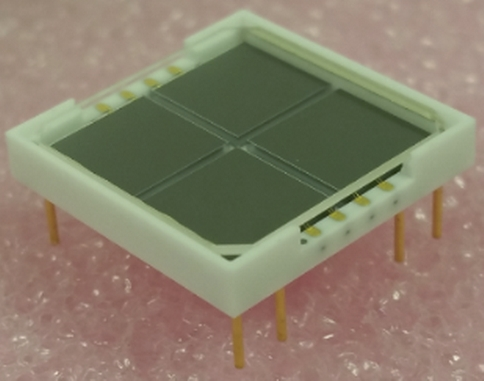
\includegraphics[width=3cm]{plots/single_mppc.jpg}
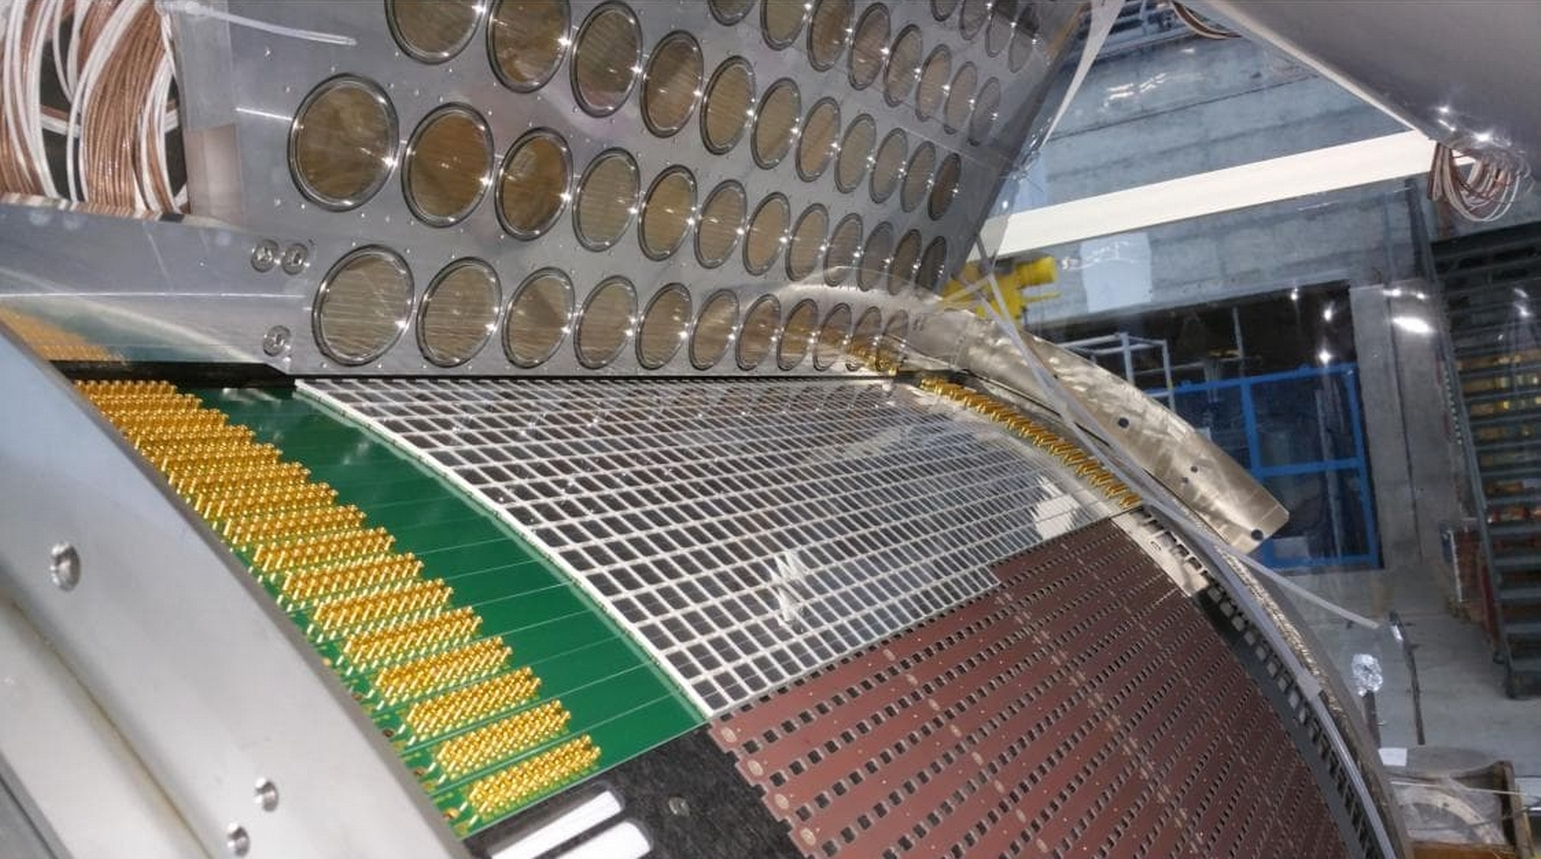
\includegraphics[width=5cm]{plots/CFRP_spacer_MPPC.jpg}
\caption{Single MPPC and installed MPPCs in the LXe calorimeter.}
\label{fig:mppc} 
\end{figure}

\begin{figure}
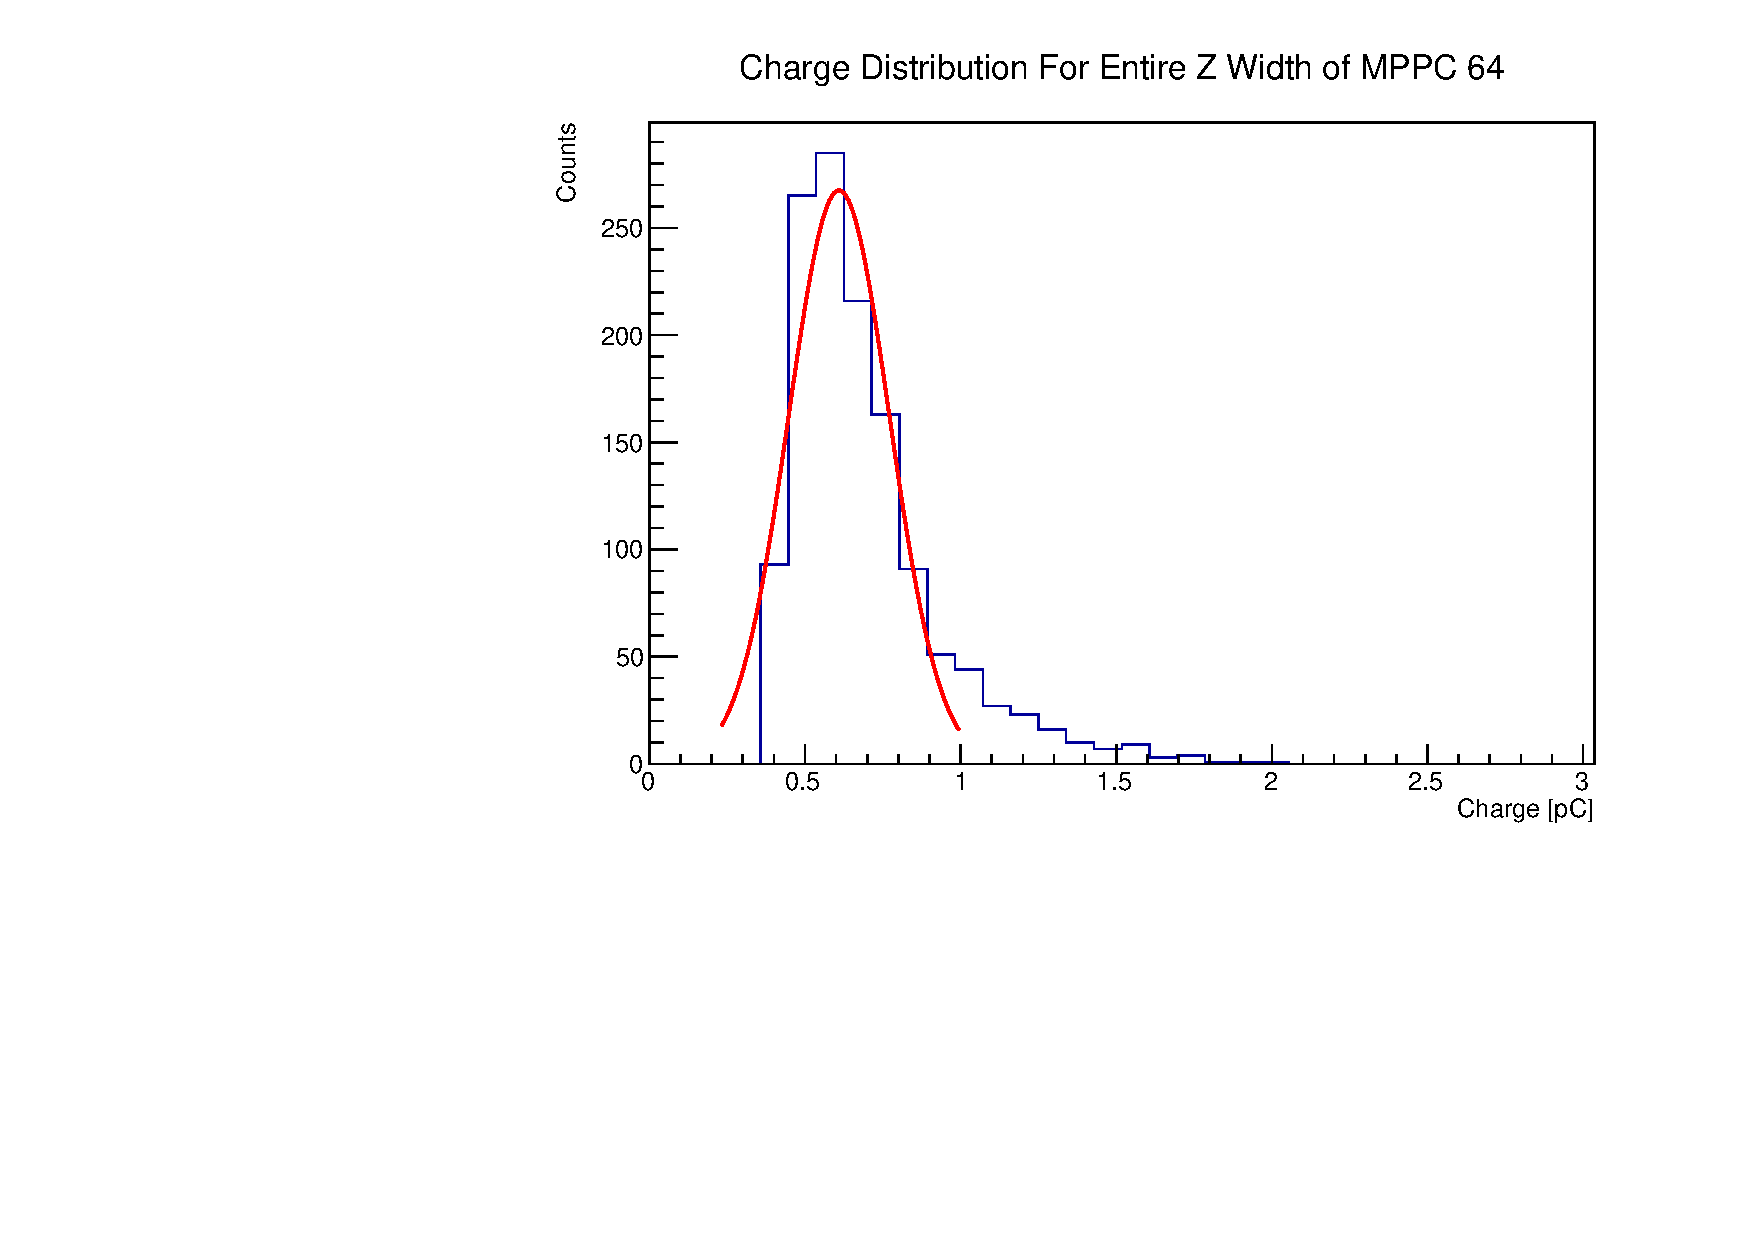
\includegraphics[width=4cm]{plots/2018/qgaindist64.pdf}
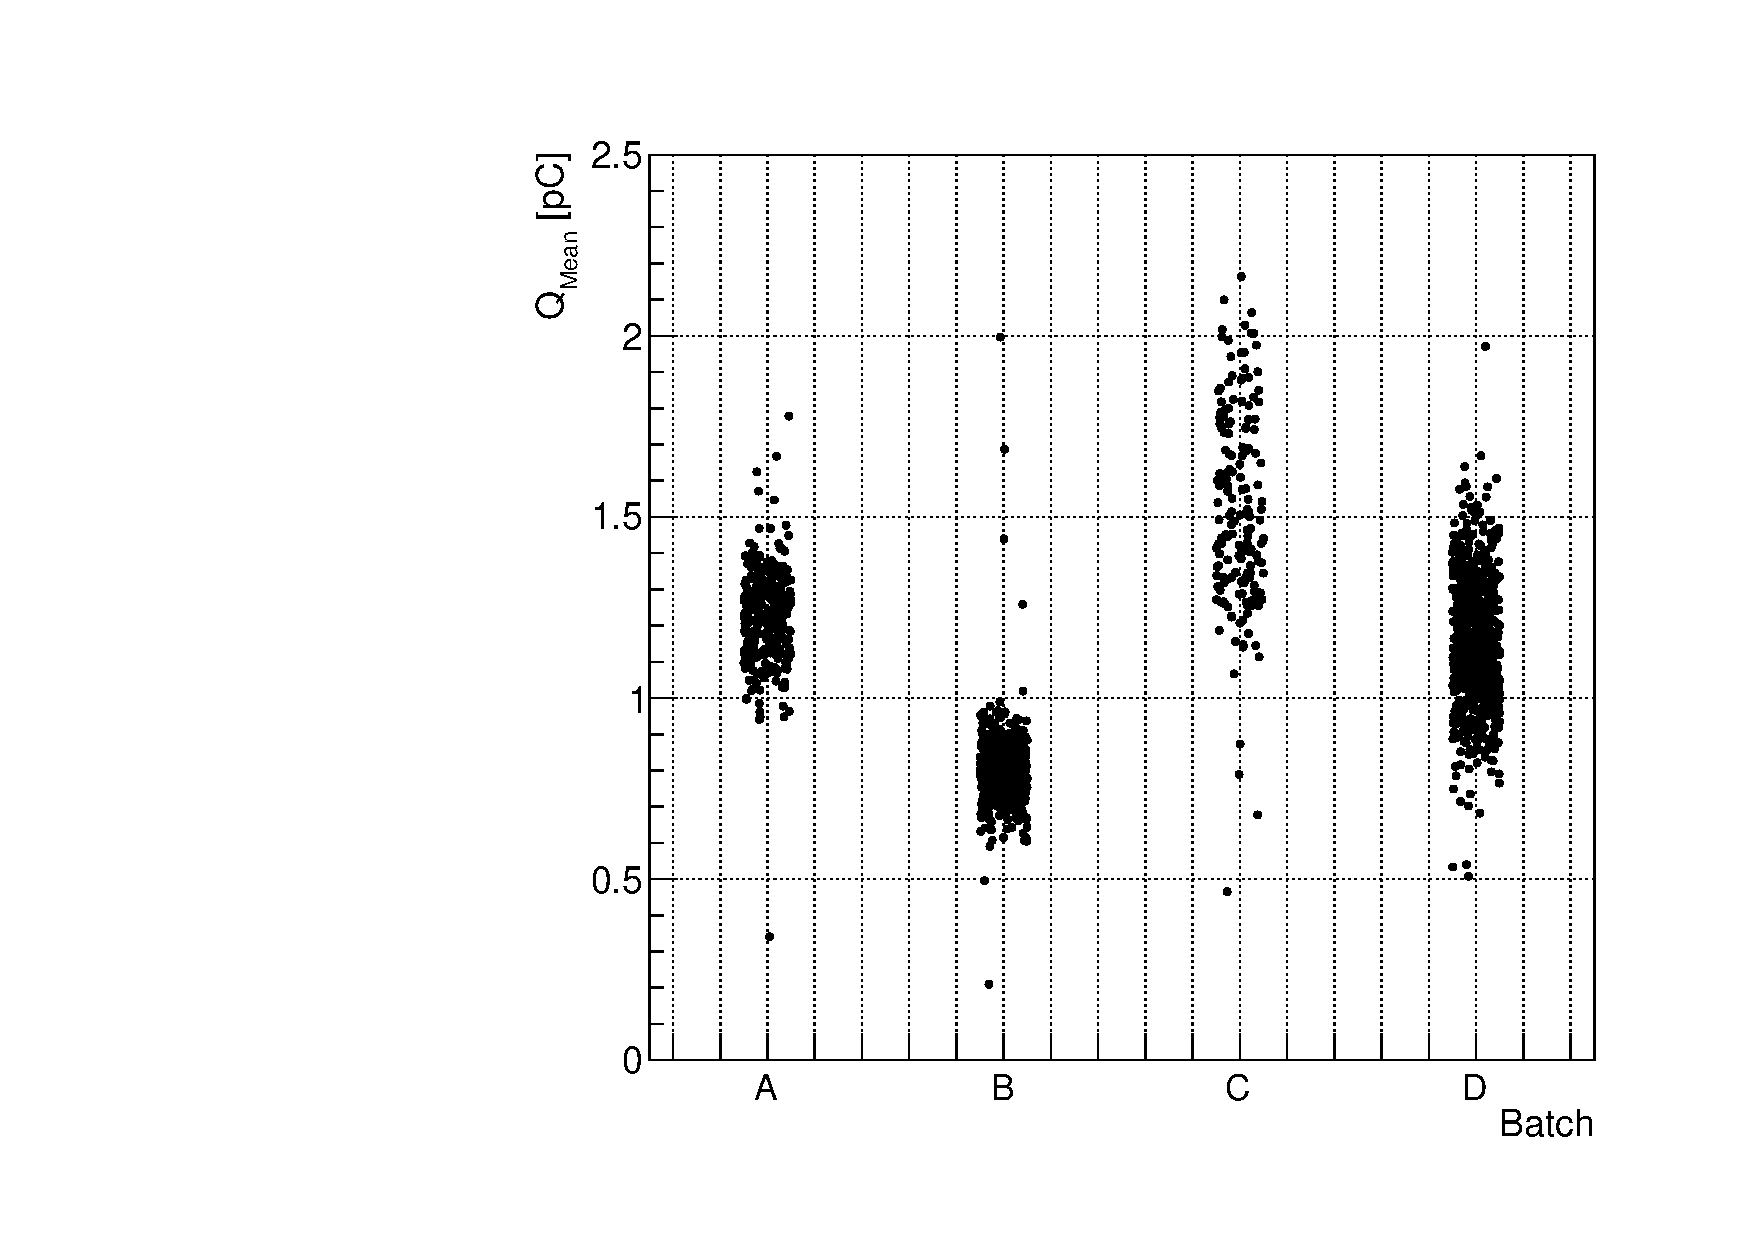
\includegraphics[width=4cm]{plots/2018/qmean_vs_batch.pdf}
\caption{Charge measured in a single MPPC with gaussian fit (left).
Mean charge measured measured in the batch (right). }
\label{fig:mppccharge} 
\end{figure}

The fine scanning resolution (scanning step 1 mm in z and \phis, and
X-ray beam size  $\sim$ 1 mm), is used to determine variation in
charge response of the component pixels of the photodetector.  The
position dependent variation in mean charge seen in figure
\ref{fig:xrayevents} demonstrates the difference in the response of
half photodetector  (two of four pixels) illuminated at every
position.  A visible decrease at the center of the photodetector is
caused by the central gap between the two rows of pixels.  Mean charge
in each half of the photodetector is independently calculated about
the center position determined in the previous analysis.  We find that
the mean charge varies between the two halves seperated by their Z
coordinate by 10\% and equal in the two halves separated by \phis.  Due
to the relative rotation the PCB strips per row about the center, the
mean charge of each half of the photodetector is also swapped
accordingly (fig \ref{fig:pixelcharge}). 
This disparity in charge response
is found to be independent of the production batch of the 
photodetector, observed at consistent level across all
batch groups.

An analysis of gain equalized charge measurements
was performed to assess its impact on the calculated 
photodetector position. There was no significant change
in the photodetector position with the resolution
degrading marginally by 0.05 mm. 

\begin{figure}
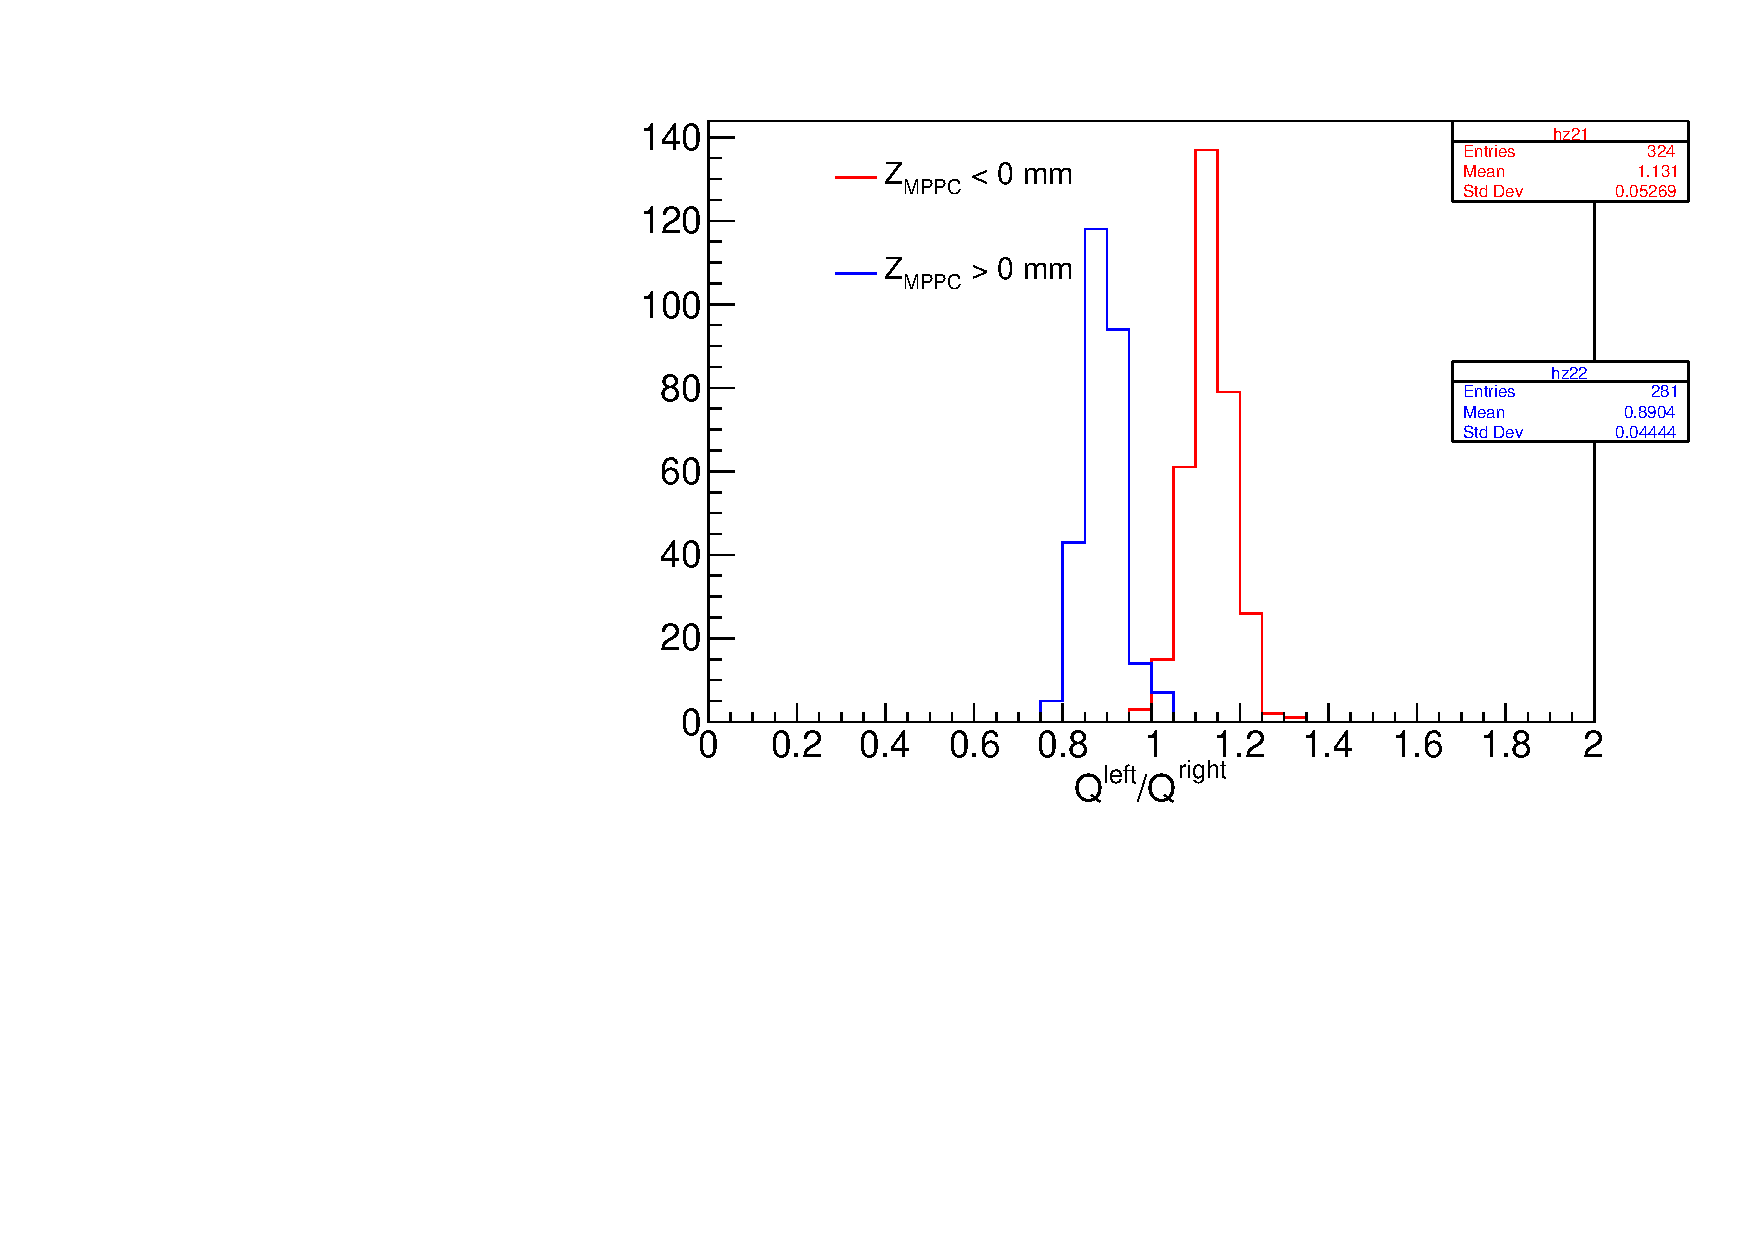
\includegraphics[width=4cm]{plots/2018/h1_z.pdf}
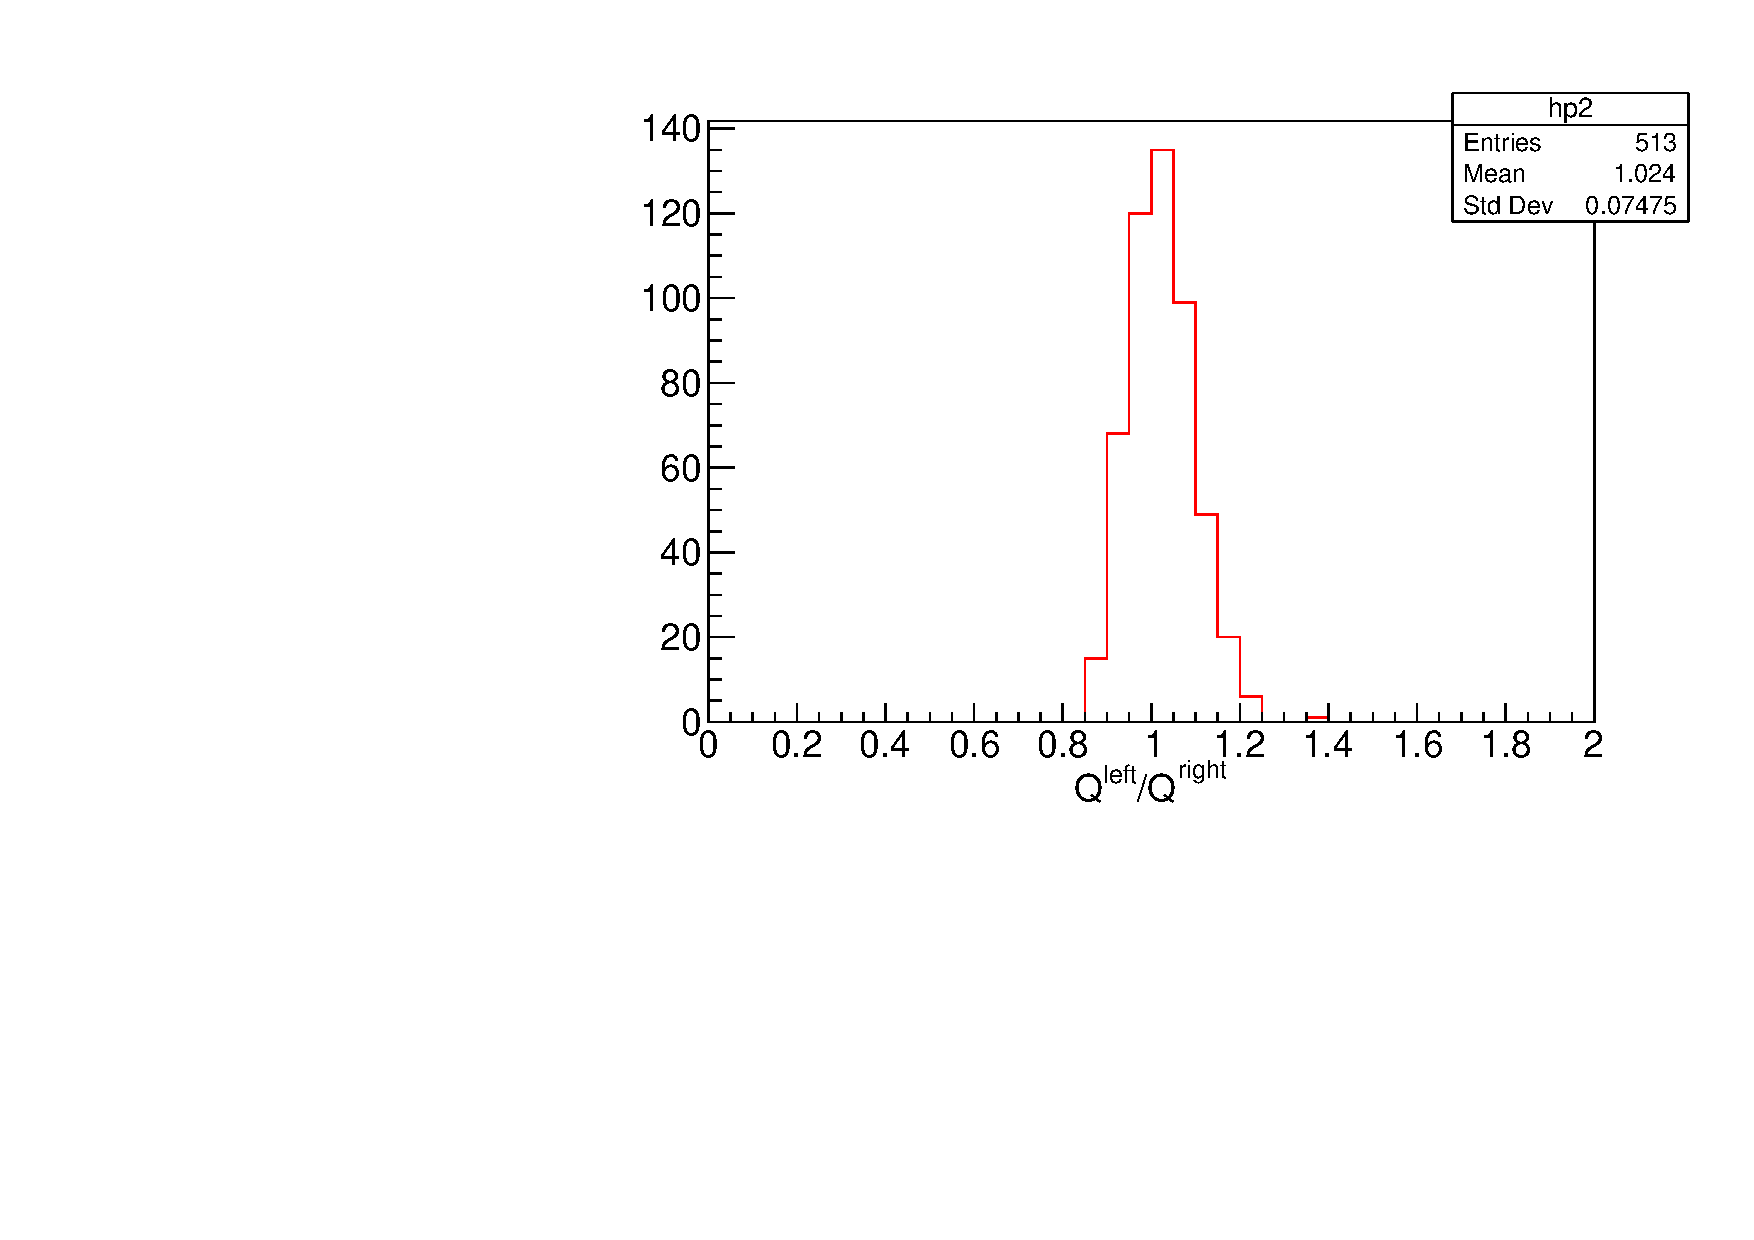
\includegraphics[width=4cm]{plots/2018/h1_phi.pdf}
\caption{Relative mean charge in positive and negative half of the 
photodetectors in z and \phis scans.}
\label{fig:pixelcharge} 
\end{figure}




\section{Ancillary Measurements}

We discuss in this section a number of ancillary measurements that are not central to the primary goal of measuring the photo-detector positions but are a valuable by-product of the x-ray position measurement technique. 

\subsection { X-ray interaction rate -- 2017 vs 2018}  
The efficacy of spacer materials between MPPC, PCB strip and CFRP
plate is tested by examining the X-ray event rate as a function of
MPPC position. The rate is inversely proportional to the length of LXe
traversed by the X-ray before interaction.  It provides crucial
information about the state of spacer materials responsible for
preventing LXe leak between inner cryostat wall and the photosensitive
surface, which directly impacts photo detection and reconstruction
efficiencies, and energy response.  A constant rate of triggered
events is expected from all scanned MPPCs with some variation
attributed to electronic readouts that are nominally configured in an
identical way.  The event rates show a $\phi$ dependent variation
indicating some deformation in CFRP plates 1 and 2.  A drop in the
rates by a factor 1/e suggests the scale of deformation
$\approx\,\lambda_{\mathrm{Xe}}$.  The $\phi$ dependent variation is
observed in both Z and $\phi$ scans in the MPPCs illuminated with
X-rays and is not seen in the background process
(Figure~\ref{fig:ratesvszphi}).  The second scan in 2018 replicates
the previous years data at a lower rate due to reduced activity of the
source by two half-lives.  
\begin{figure}[]
\centering 
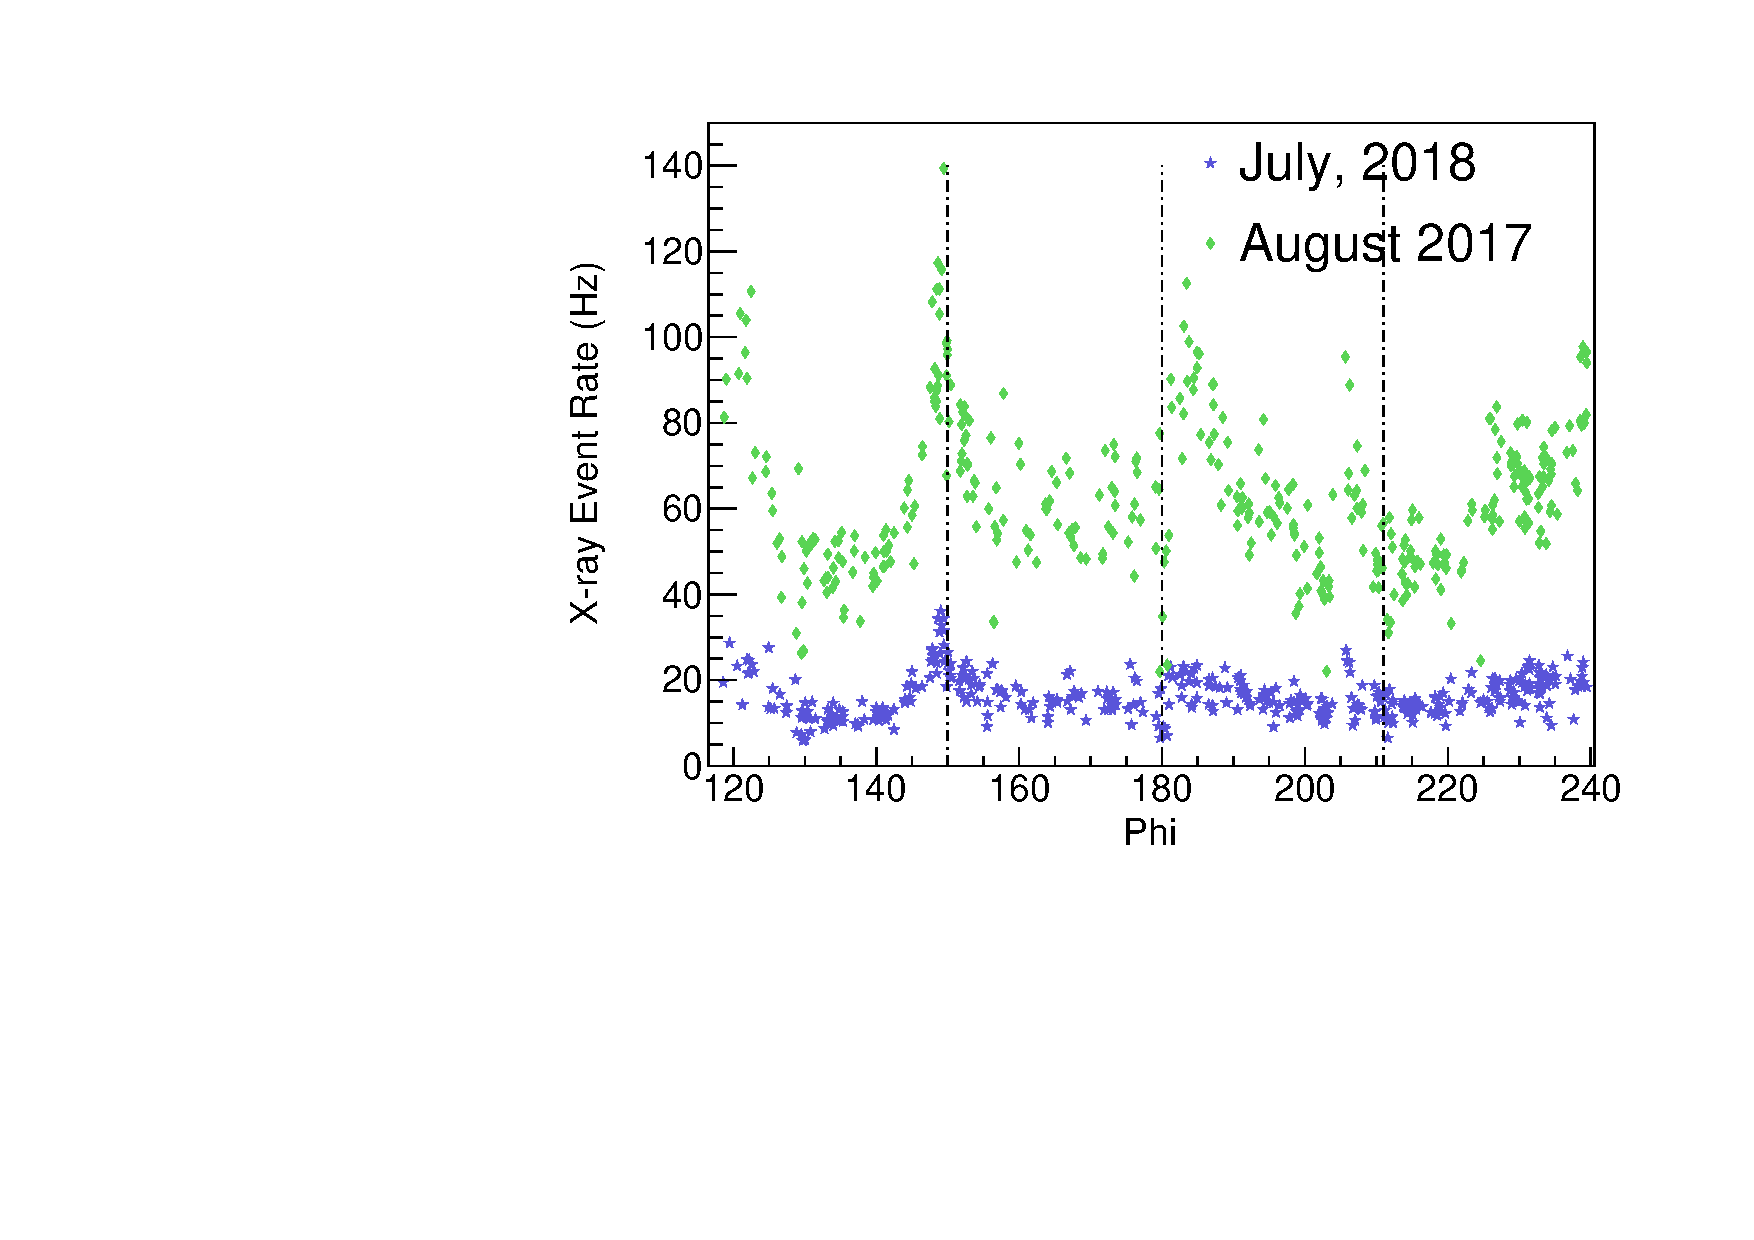
\includegraphics[width=4cm]{plots/2018/cEventRate_1718}
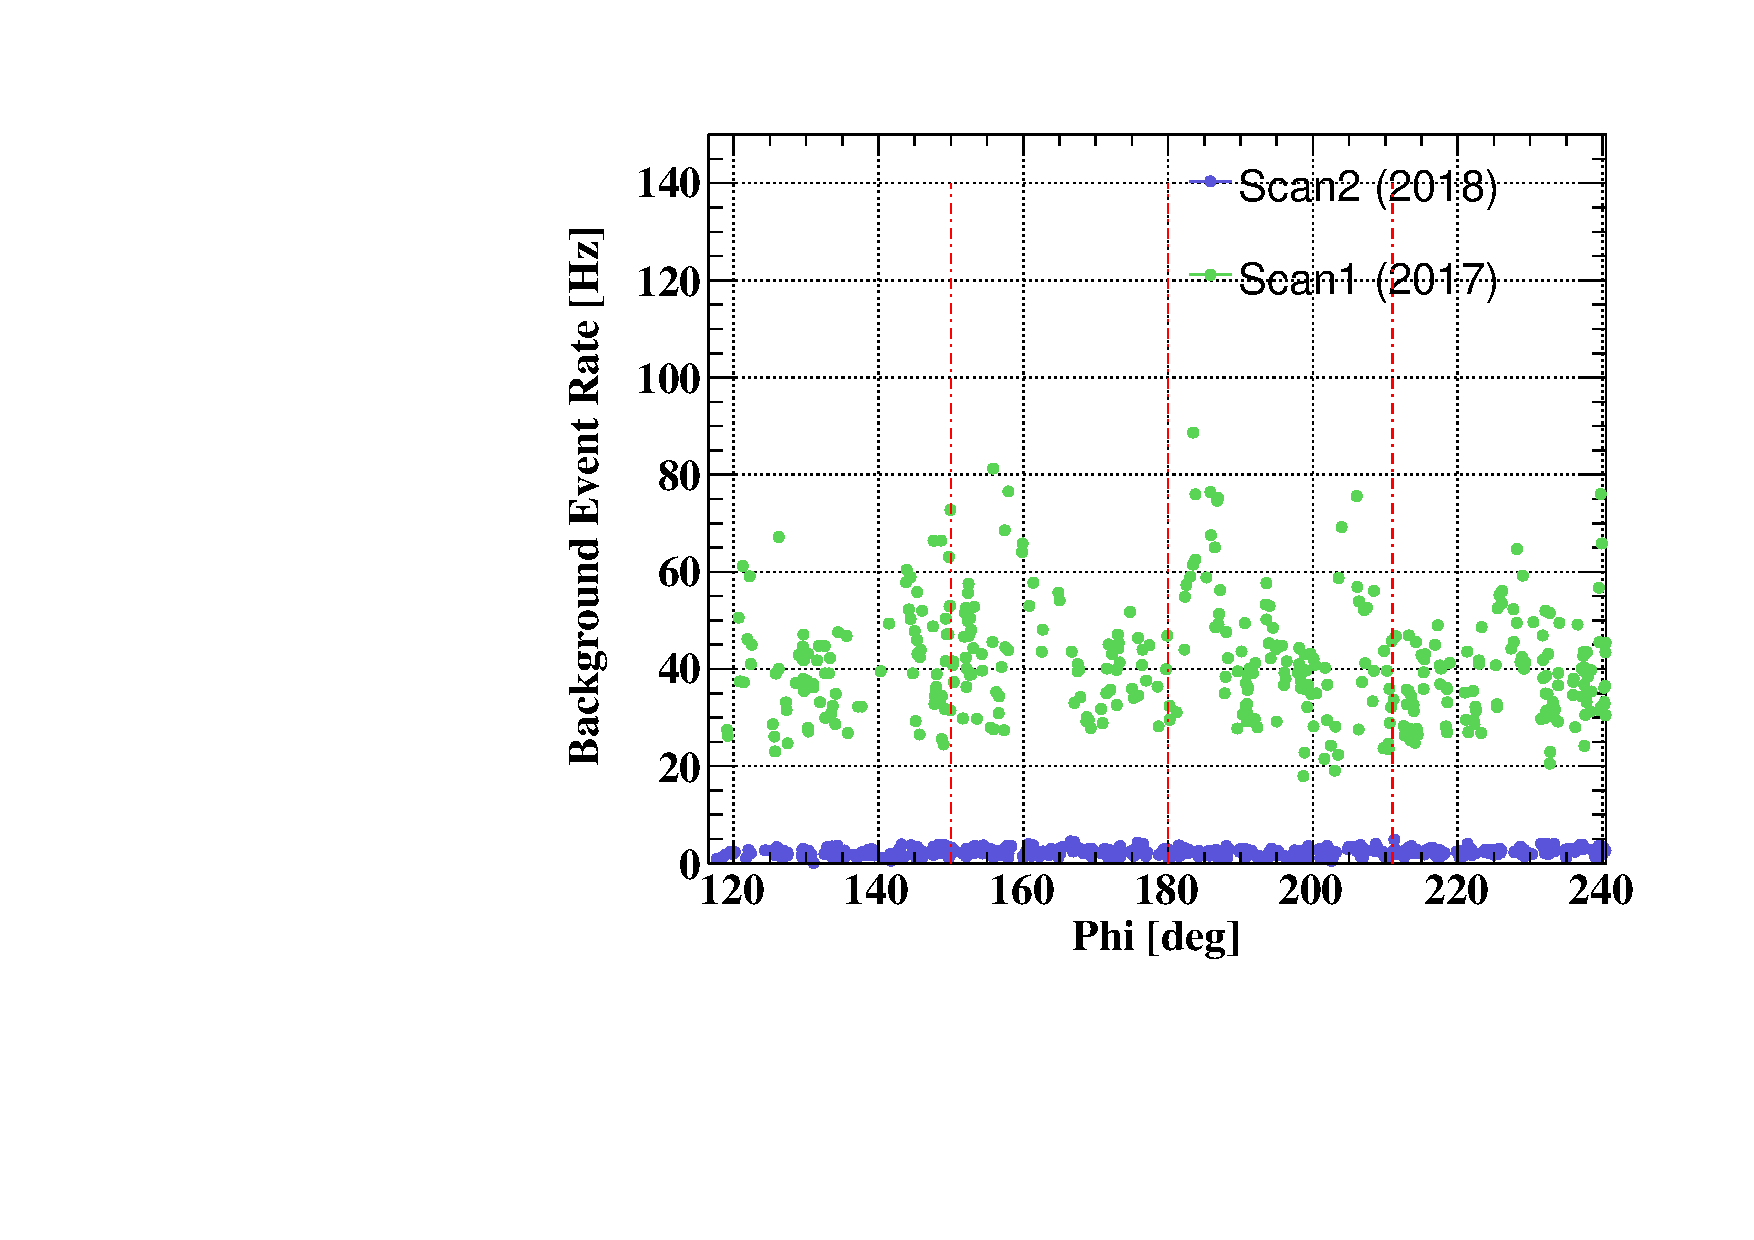
\includegraphics[width=4cm]{plots/2018/cBkgRate_1718} \\
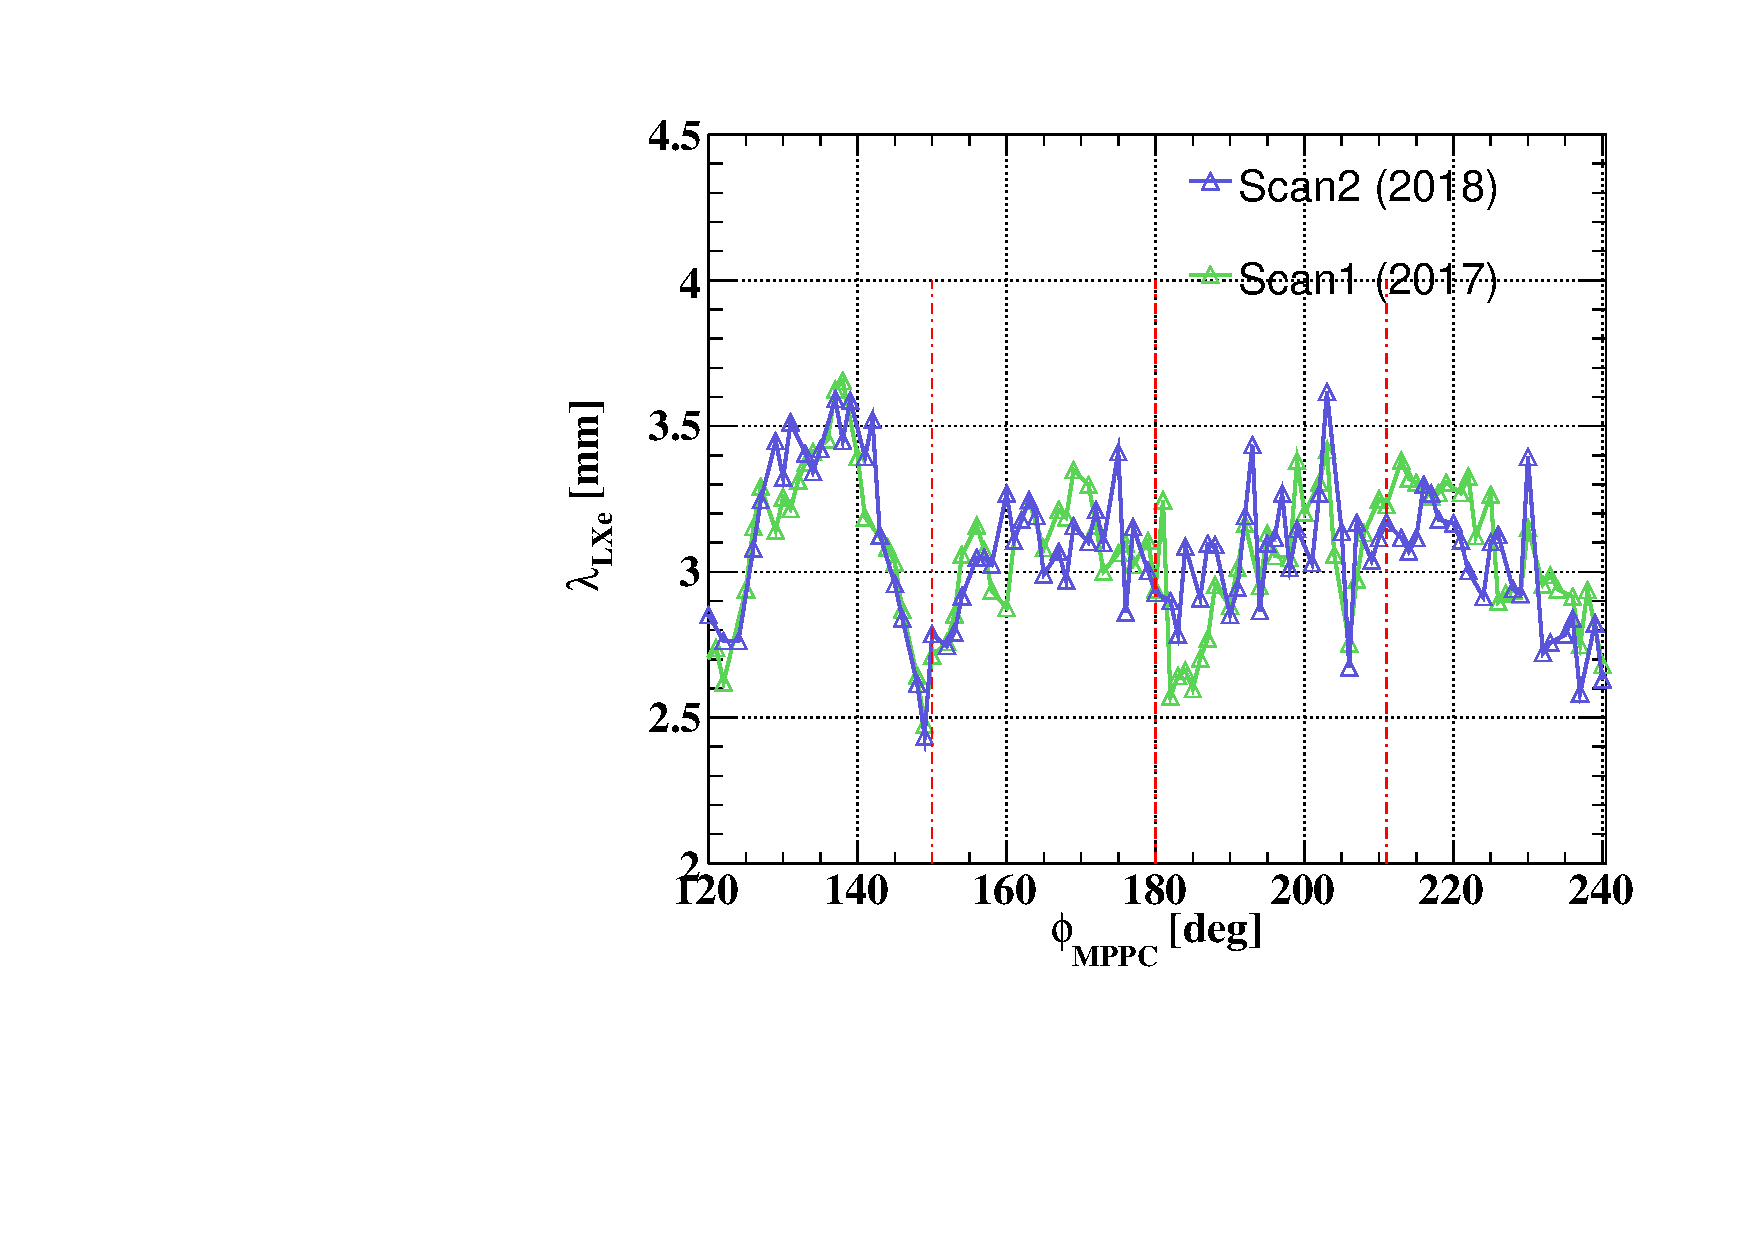
\includegraphics[width=4cm]{plots/2018/AbsorptionLength} 
\caption{Signal and background trigger rates observed in MPPC as a function of $\phi$.
Red dashed lines indicate the edges of the CFRP plate.}
\label{fig:ratesvszphi} \end{figure}


\subsection{Quantum Efficiency$\times$Gain}\label{sec:qegain}
\begin{comment}



\textbf{ADD REFERENCE TO SECTION3: MPPC STRUCTURE, CALORIMETER, 
SECTION6: INITIAL MPPC SCAN}\\
\end{comment}
In this section, we discuss our found charge gains between the individual MPPCs and between the four production batches in which we sourced the MPPCs.

Utilizing the collimated X-ray beam as a uniform light source, the mean charge
response is measured across the 12mm face of individual mppcs 
%, proportional to the gain and quantum efficiency, 
 The mean charge response
then serves as a measure of the relative gain$\times$QE between photodetectors
in the scanned region of the calorimeter. % It must be noted
%that the charge measurement contains smaller but inseparable
%contributions from after-pulse and cross-talk between neighboring
%photodetectors, which are independent from the photodetector gain.
Only relative measurements of gain are possible as the
absolute photon yield in the X-ray interaction relies on other factors
such as presence of impurities in the liquid Xenon which were not
precisely known. 

\begin{comment}
The photodetectors are developed according to the experimental
requirements with large photosensitive area 12 $\times$ 12 mm$^2$,
comprised of four  smaller pixels 6 $\times$ 6 mm$^2$ connected in
series.  The photodetectors are placed in a ceramic case (15 mm) and
mounted on a PCB strip, each containing 22 photodetectors.  Two
identically produced strips aligned along $\hat{z}$ direction, and
rotated by 180\degree with respect to each other to allow for
electronics readout at each end, make up a single row (fig 
\ref{fig:mppc}).
\end{comment}

%The mean charge  is calculated over the 12 mm region centered at the
%fitted photodetector location from previous analysis.  Due to long
To reduce the impact of high energy tails
in the charge distribution, the mean is measured using an iterative Gaussian fit; the
initial fit covers the entire range and then the fit range is restricted to the two sigma
region of the first fit.  Fig. \ref{fig:mppccharge} shows these mean charges vary overall between the
scanned photodetectors by 50\%, and correlate reliably with the
production batch of the photodetectors (fig \ref{fig:mppccharge}). 

\begin{figure}
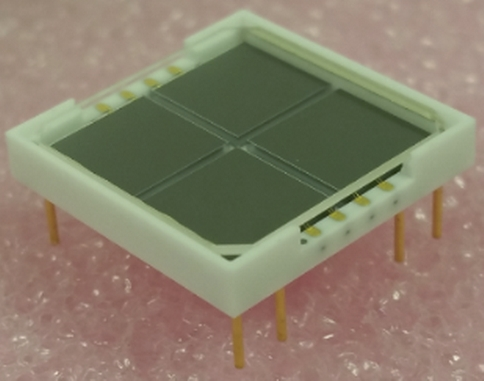
\includegraphics[width=3cm]{plots/single_mppc.jpg}
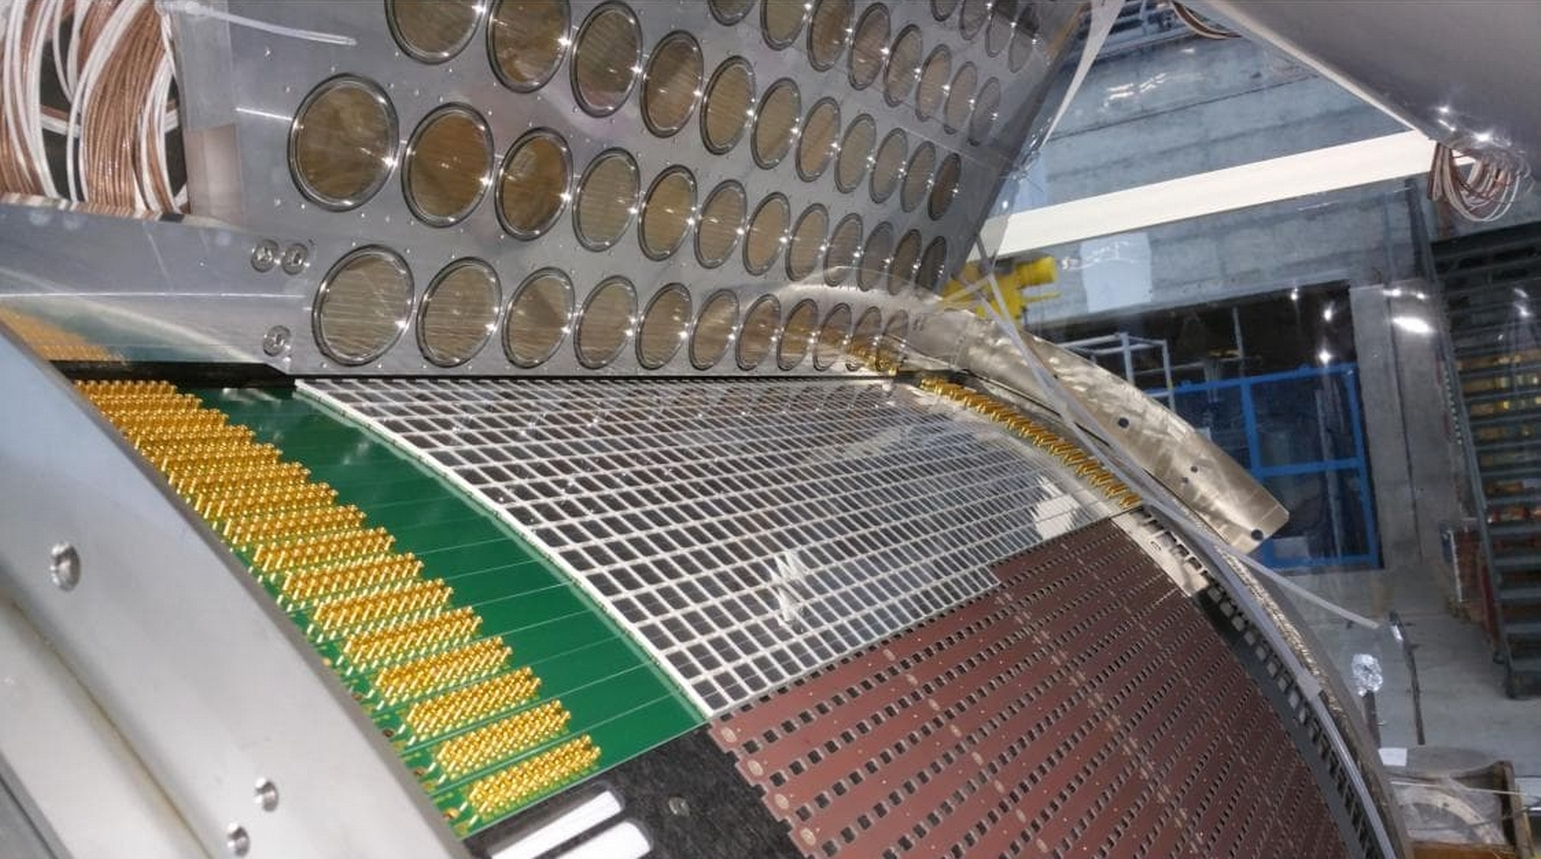
\includegraphics[width=5cm]{plots/CFRP_spacer_MPPC.jpg}
\caption{Single MPPC and installed MPPCs in the LXe calorimeter.}
\label{fig:mppc} 
\end{figure}

\begin{figure}
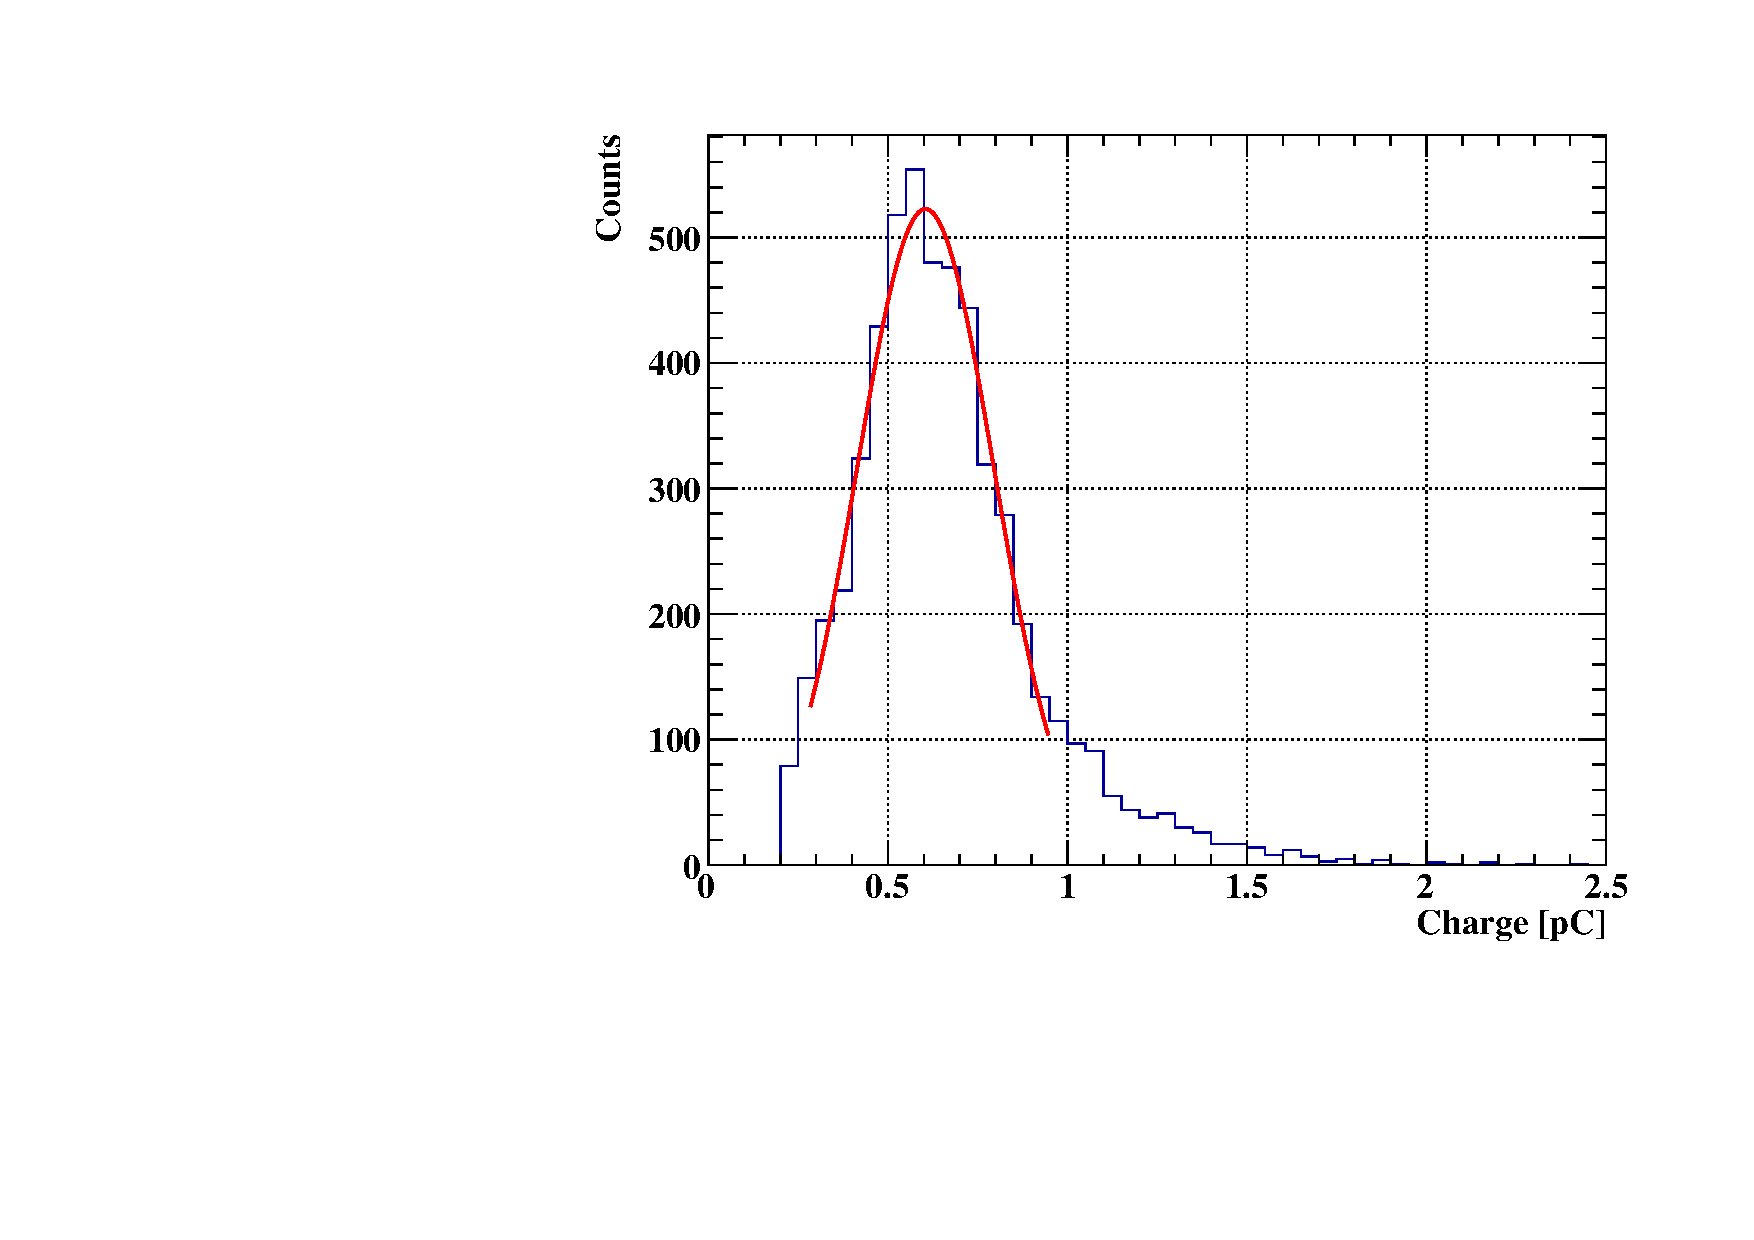
\includegraphics[width=4cm]{graphics/q64fit.pdf}
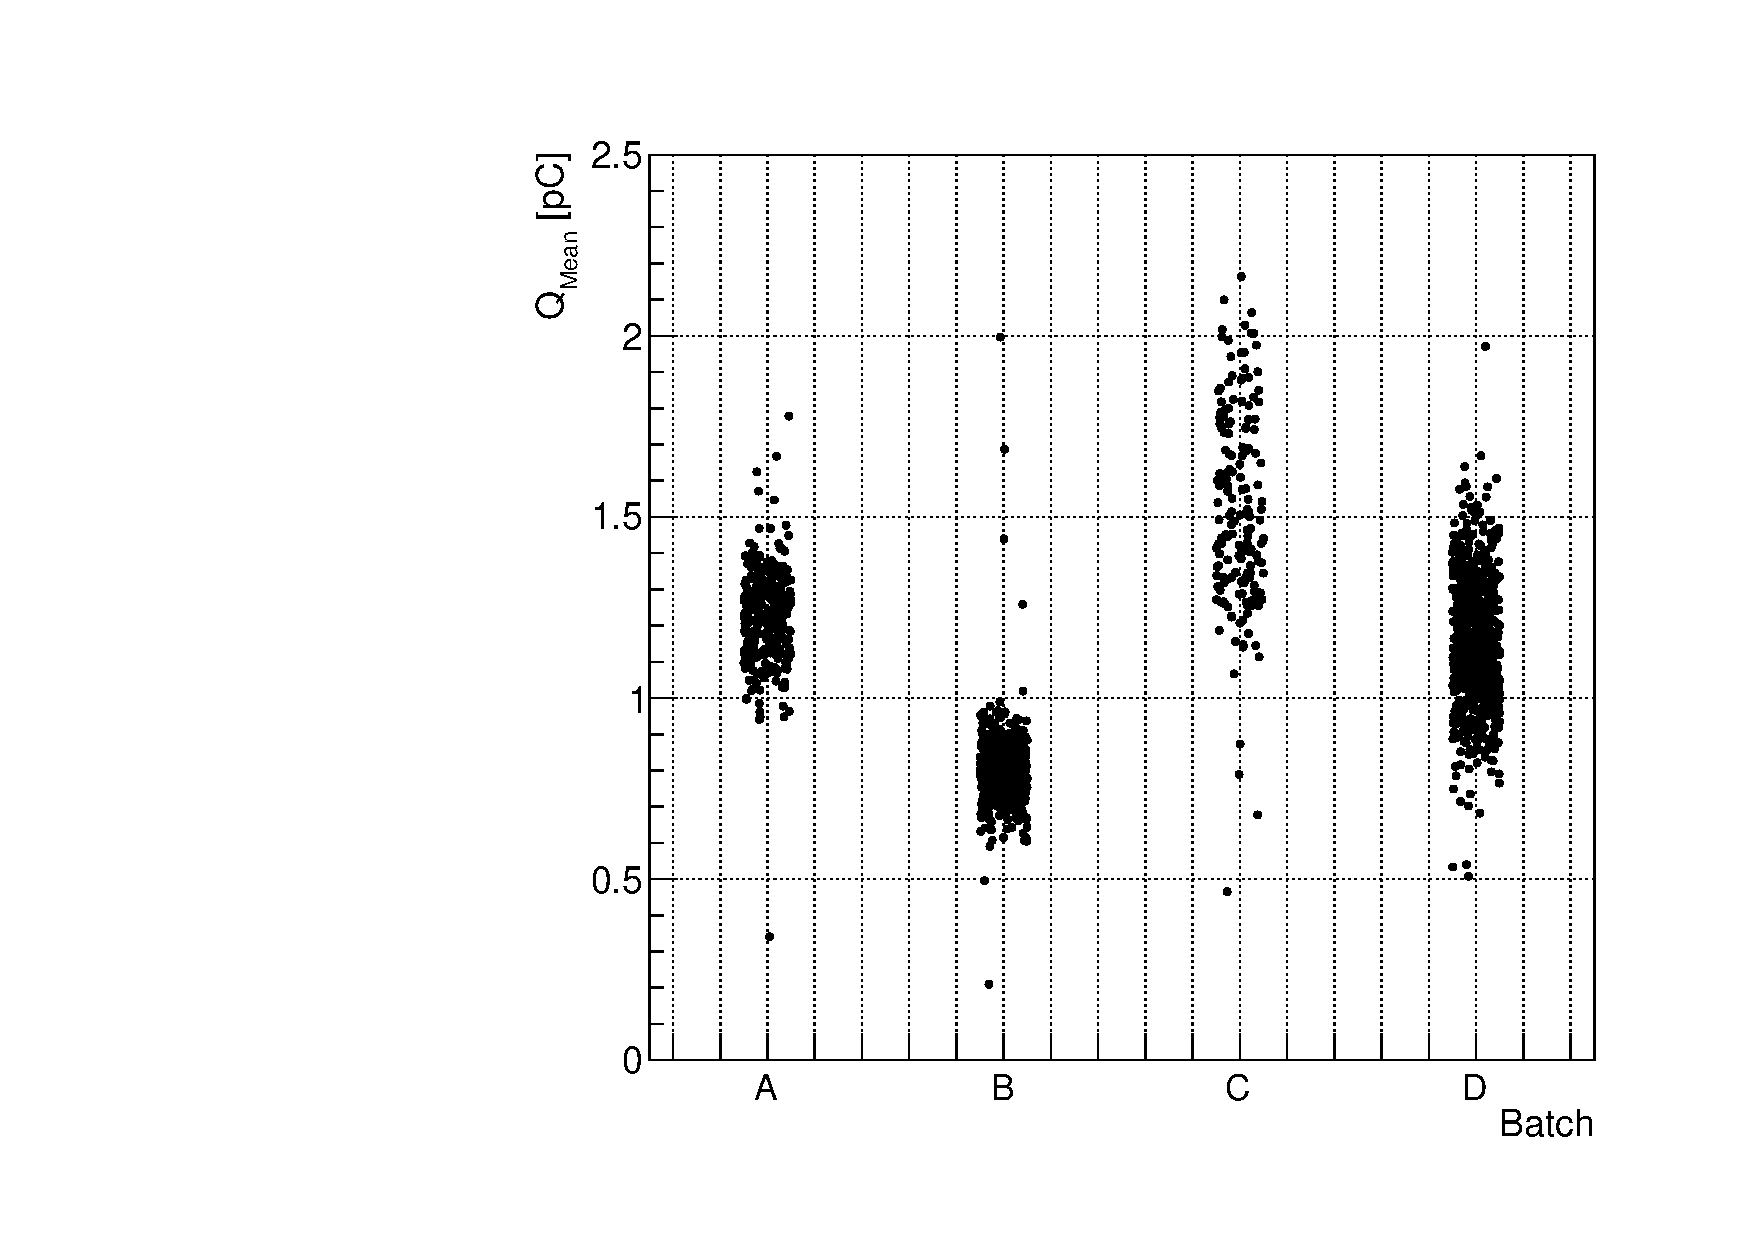
\includegraphics[width=4cm]{plots/2018/qmean_vs_batch.pdf}
\caption{Charge measured in a single MPPC with gaussian fit (left).
Mean charge measured measured in the batch (right). }
\label{fig:mppccharge} 
\end{figure}


\subsection{Sub-MPPC/Quadrant Gain}
Furthermore, we describe here variations in gain across the active area of individual photodetectors.

The fine scanning resolution (scanning step 1 mm in z and \phis, and
X-ray beam size  $\sim$ 1 mm), is used to determine variation in
charge response of the component pixels of the photodetector.  The
position dependent variation in mean charge seen in figure
\ref{fig:xrayevents} demonstrates the difference in the response of
half photodetector  (two of four pixels) illuminated at every
position.  A visible decrease at the center of the photodetector is
caused by the central gap between the two rows of pixels.  Mean charge
in each half of the photodetector is independently calculated about
the center position determined in the previous analysis.  We find that
the mean charge varies between the two halves seperated by their Z
coordinate by 10\% and equal in the two halves separated by \phis.  Due
to the relative rotation the PCB strips per row about the center, the
mean charge of each half of the photodetector is also swapped
accordingly (fig \ref{fig:pixelcharge}). 
This disparity in charge response
is found to be independent of the production batch of the 
photodetector, observed at consistent level across all
batch groups.

\begin{figure}
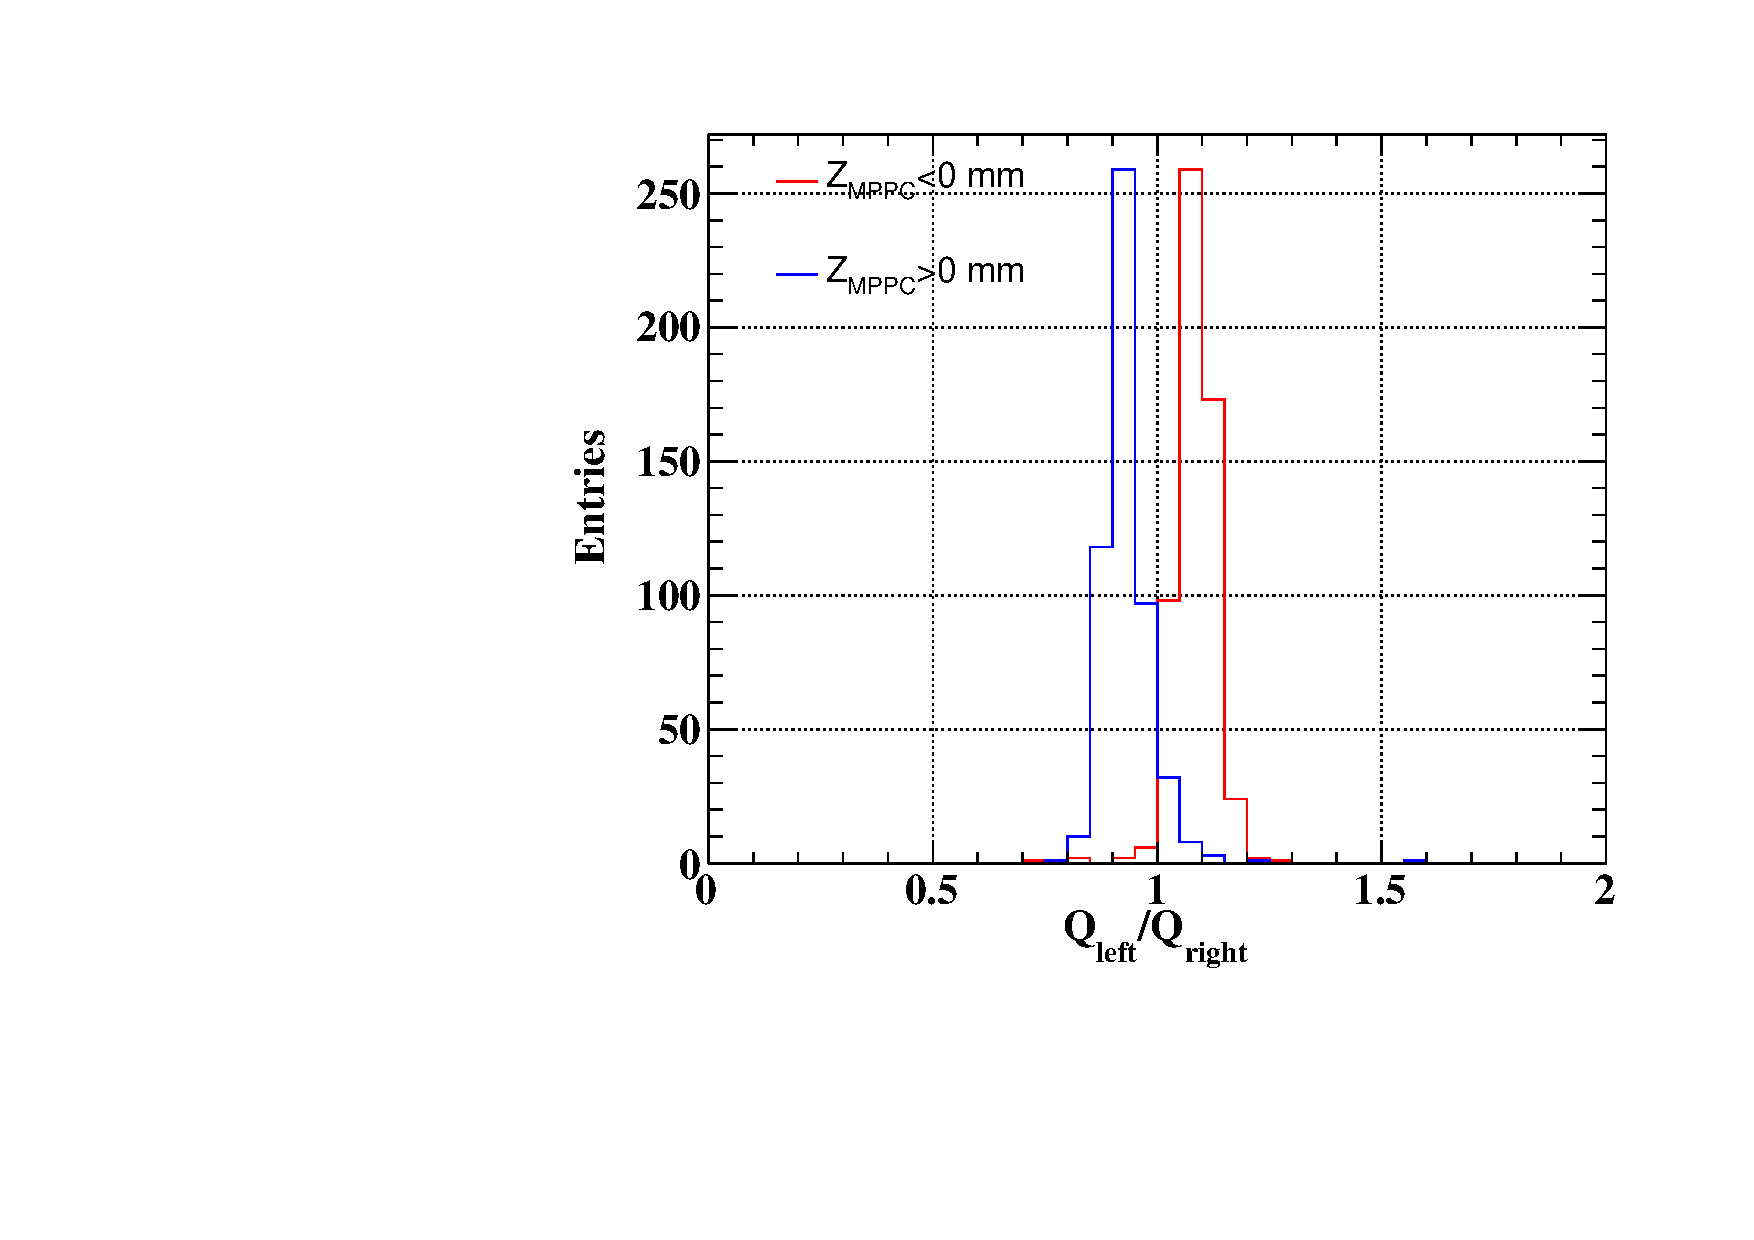
\includegraphics[width=4cm]{plots/2018/qratio_z_wf.pdf}
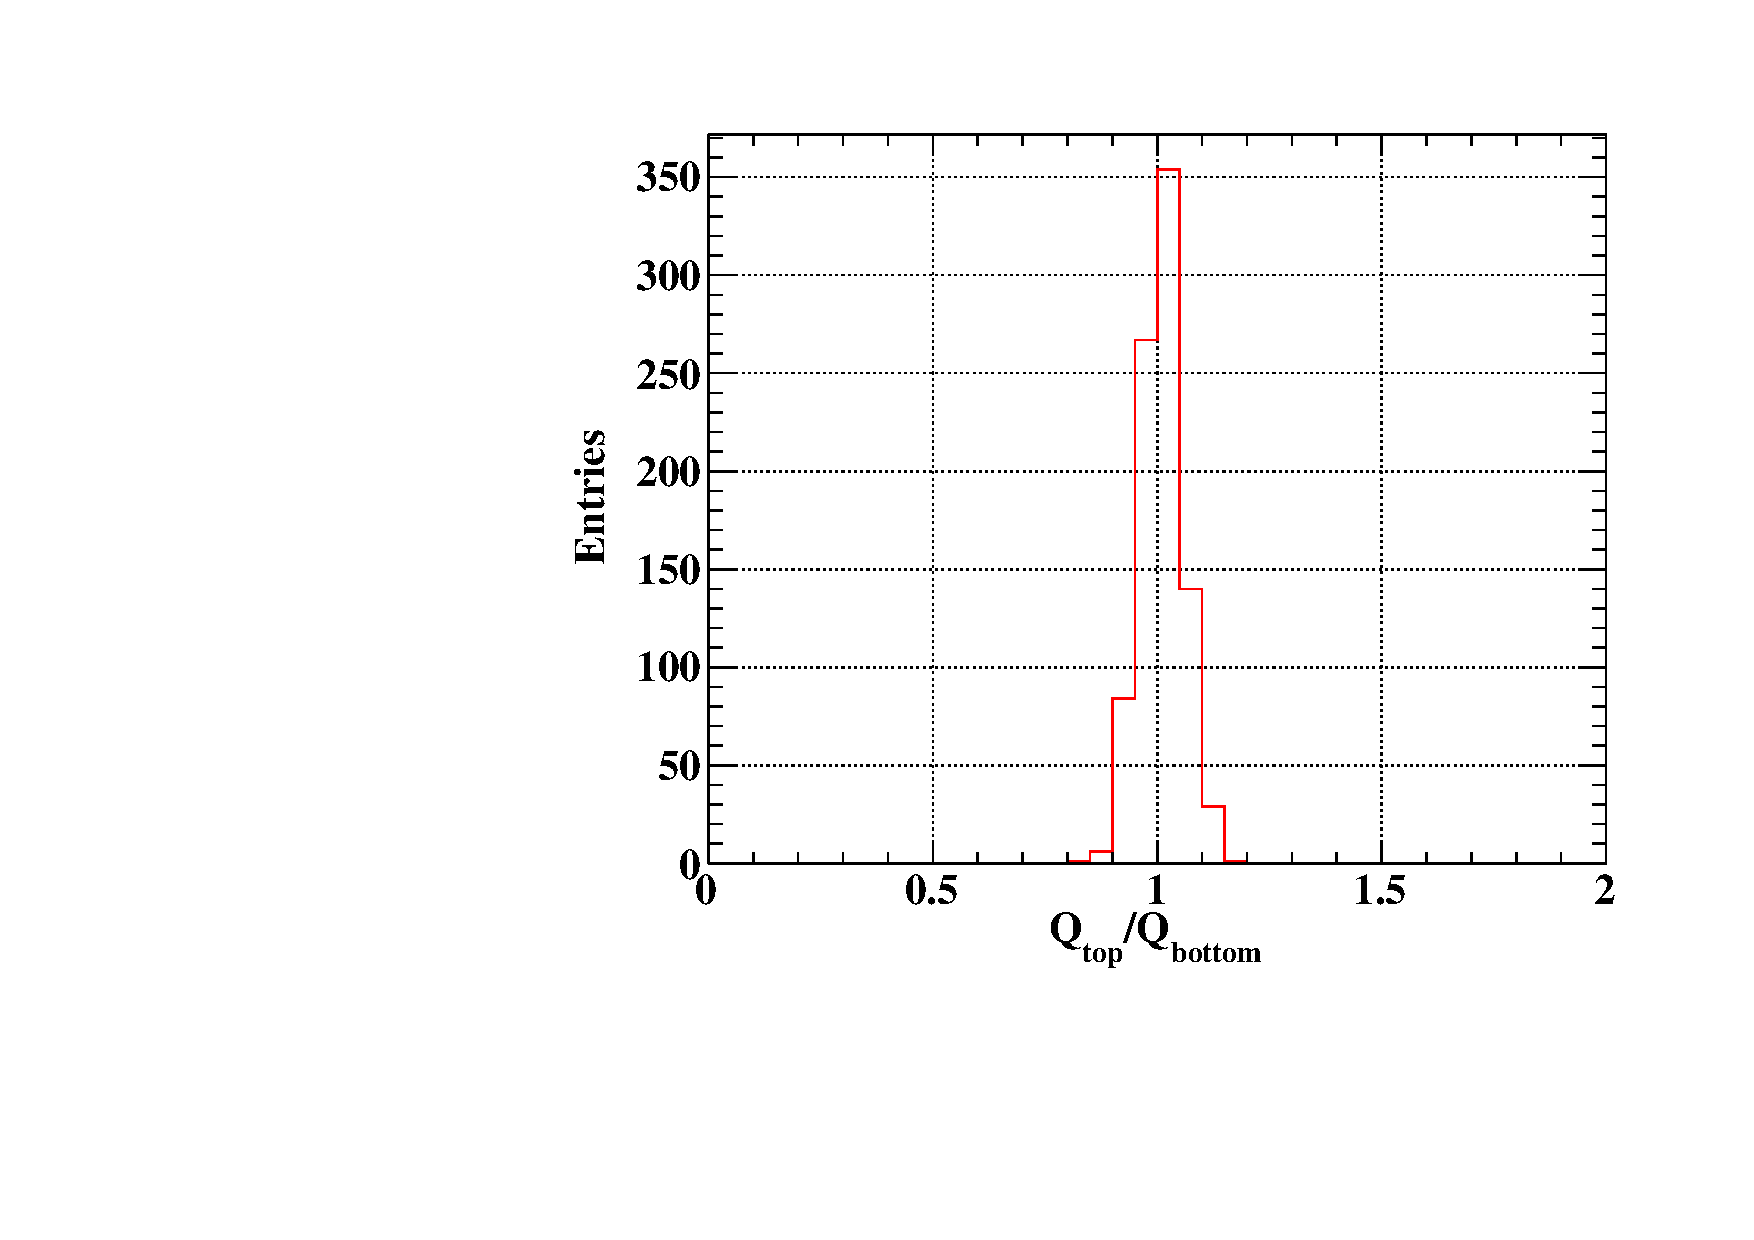
\includegraphics[width=4cm]{plots/2018/qratio_phi_wf.pdf}
\caption{Relative mean charge the two halves of the 
photodetectors in the scanning direction.}
\label{fig:pixelcharge} 
\end{figure}






\section{\label{conclusion}Conclusion}
A novel approach for position survey of photodetectors and its
application to the LXe calorimeter of the MEG experiment is described.
It is performed using a collimated and precisely controlled X-ray beam
to scan photodetectors in an optically opaque cryostat subject to
mechanical stress and motion.  The photodetectors in the central axial
region $|Z|<120$~mm on the entrace face of the calorimeter are scanned
with average precision of 0.17~mm (0.3~mm for the region $|Z|<150$~mm)
in the axial (Z) and azimuthal ($\phi$) coordinates, outperforming the
resolution goals of the upgraded experiment.  The position map
produced as a result shows systematic displacement and, installation
artifacts observed in the form of rotation and deformation of the CFRP
assembly boards, compared to the nominal grid pattern of the
photodetectors.  Photodetectors in the outer axial region
$|Z|>150$~mm, approximately 54\% of the total, were excluded due to
high X-ray absorption by the magnet.  The calculated absolute
positions serve as a critical input for photon reconstruction in
physics analysis.  This study presents a successful implementation of
the X-ray survey technique in the MEG experiment. It demonstrates a
model for performing systematic position survey of photodetectors in
other scenarios where optical survey methods are not viable or
applicable.


\bibliographystyle{unsrt}
\bibliography{main}

\appendix
\section{Selection}
\begin{table}[H]
    \centering
    \begin{enumerate}
    \item Integrated Charge $>$ 0.6 pC
    \item Sum Trigger Waveform Peaktime $\in$ (-0.7 $\mu s$,-0.5 $\mu s$)
    \item Average Charge In Background Channels $<$ 0.2 pC
    \end{enumerate}
    \caption{Integrated Charge Based Selection Criteria}
    \label{tab:my_label}
\end{table}

\begin{table}[H]
    \centering
    \begin{enumerate}
    \item Pulse Height $>$ 50 mV
    \item Sum Trigger Waveform Peaktime $\in$ (-0.7 $\mu s$,-0.5 $\mu s$)
    \item Average Charge In Background Channels $<$ 0.2 pC
    \end{enumerate}
    \caption{Pulse Amplitude Based Selection Criteria}
    \label{tab:my_label}
\end{table}
All charge values are gain corrected by direct measurement or by measured mean of production lot if direct measurement isn't possible.

\subsection{Integrated Charge vs. Pulse Amplitude}
Here we have compared the impact of placing a threshold on two alternate attributes of the individual MPPC signal waveforms -- maximum pulse height and integrated charge under the waveform pulse. We used a fit of the interpolated FARO grid for all 4092 MPPC positions (uncertainties on these positions are much less than required for our 1 mm bin size) in order to combine scan data from all Z-Scanned MPPCs. Shown in , we find that while there is the expected, high correlation between amplitude and charge, the width of this uncertainty is perhaps larger that was anticipated. Therefore, despite the values of our two cuts being roughly equivalent on average, the width of this distribution still allows for significant differences in event selection.

\begin{figure}
    \centering
    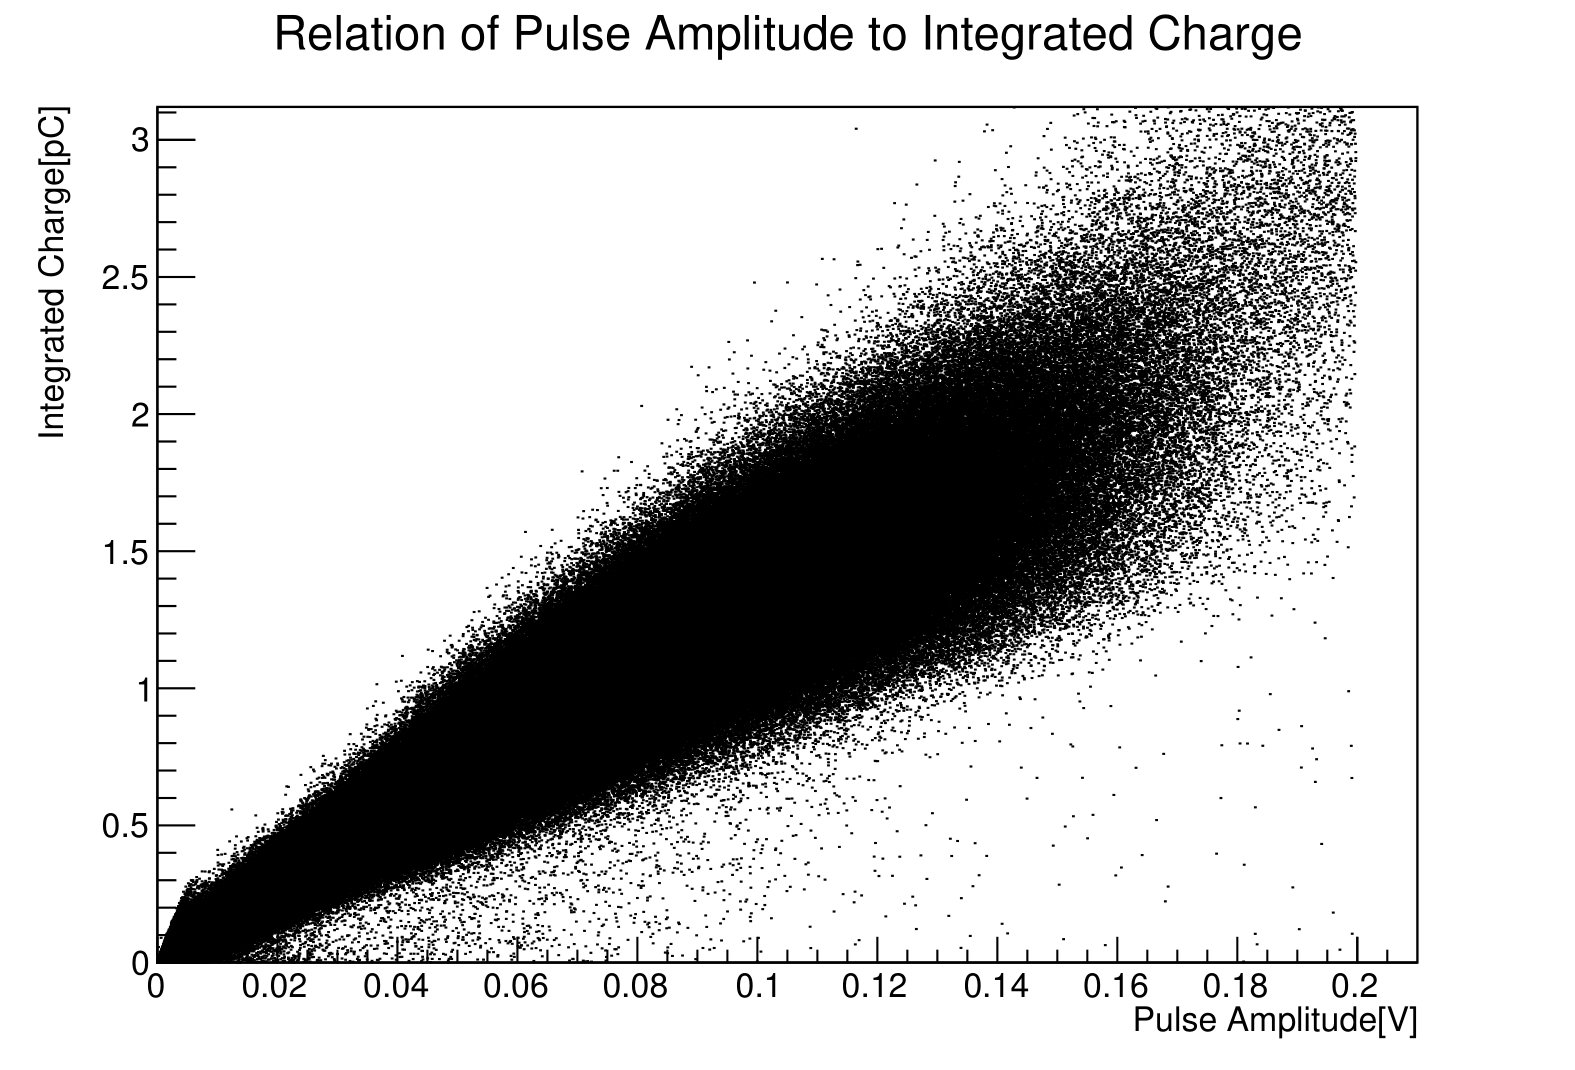
\includegraphics[width=5cm]{graphics/qvamp-1.png}
    \caption{Relationship of height to charge in a single event waveform}
    \label{fig:qvsamp}
\end{figure}

Particularly of note is that there are significant differences in this relation across the face of individual MPPCs.
Figure \ref{fig:heightvzplot} shows this via the net average mppc charge and height behaviour v. position across all scanned mppcs.
From a polynomial fit of both of these figures, we find, as agrees with prior findings, that the peaks of the charge measurements agree with our previous results of a 10\% drop in the downboard half. For height, the same effect still appears but to a much lesser extent.

\begin{figure}
\centering

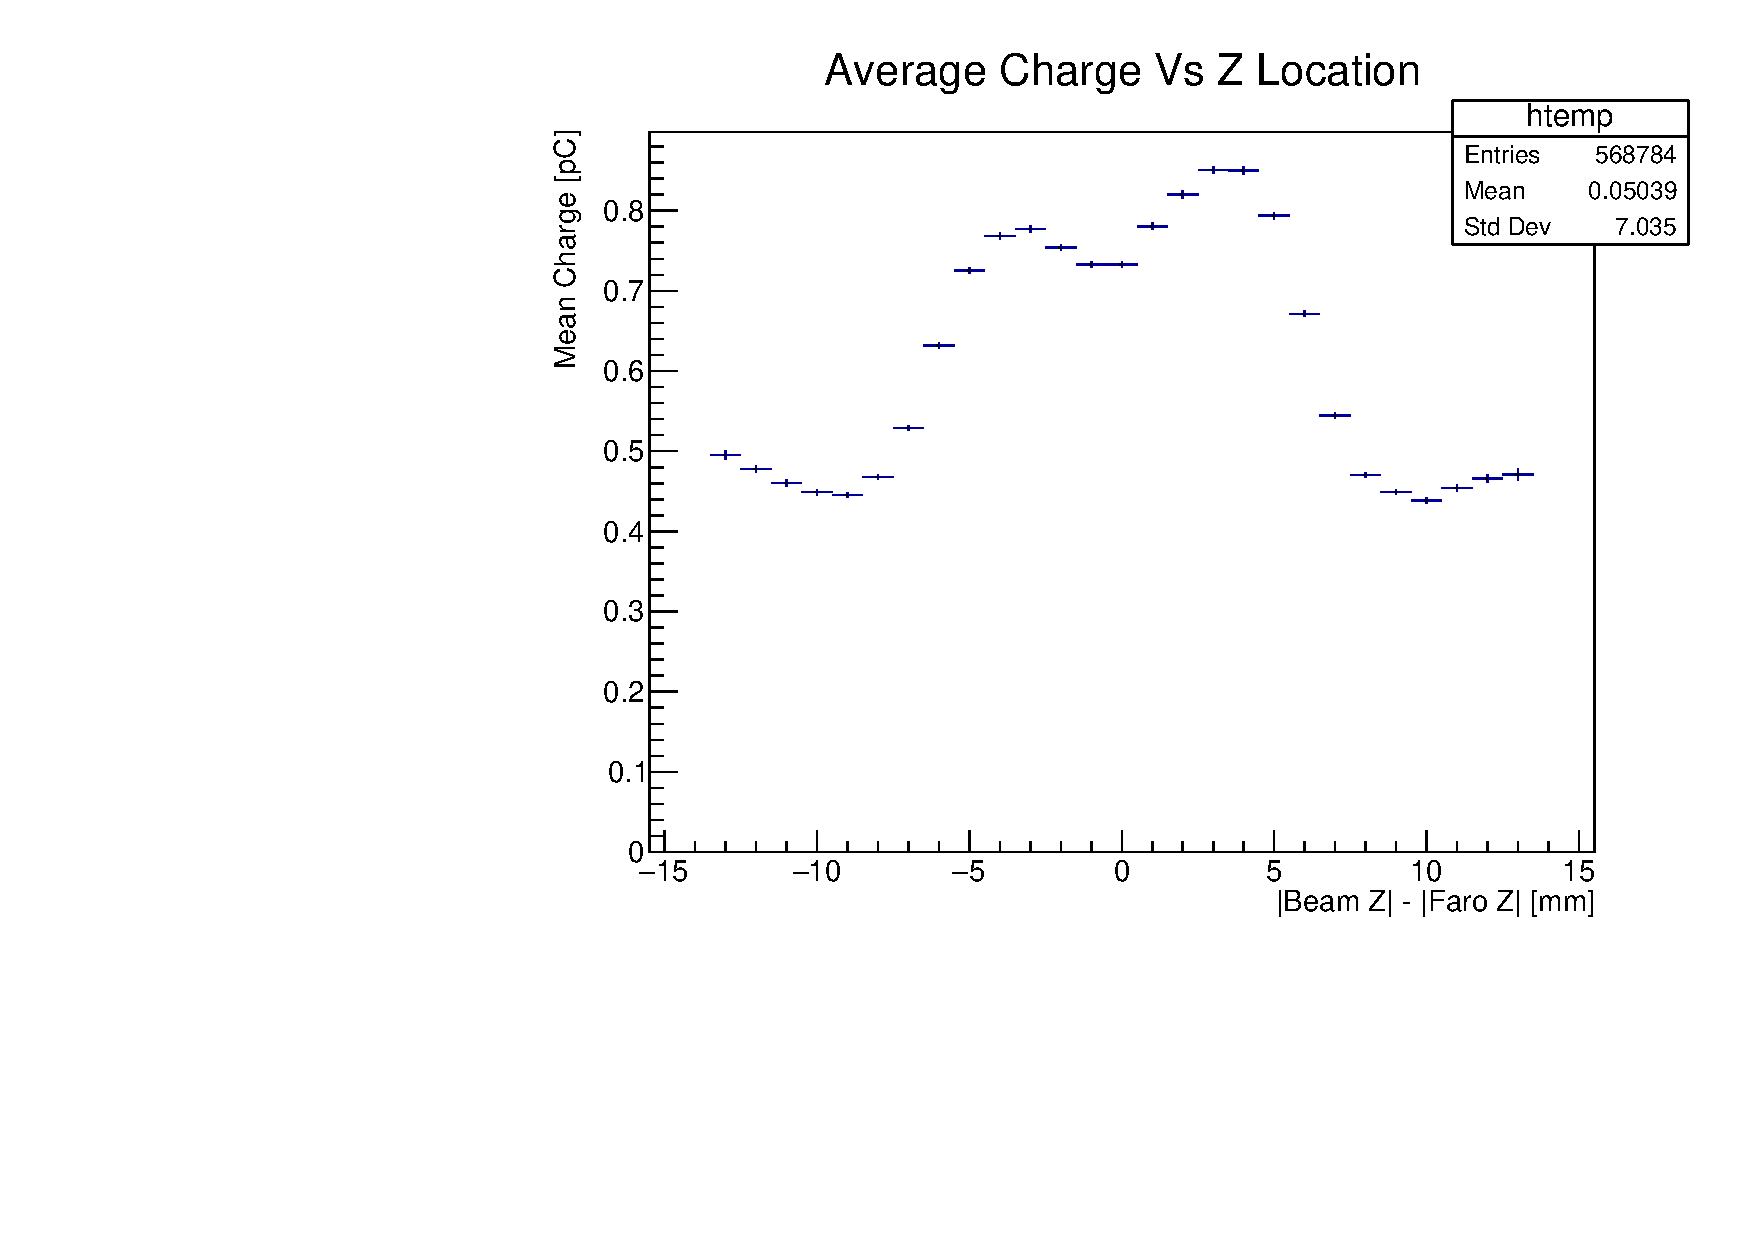
\includegraphics[width=4 cm]{graphics/chargevsz.pdf}
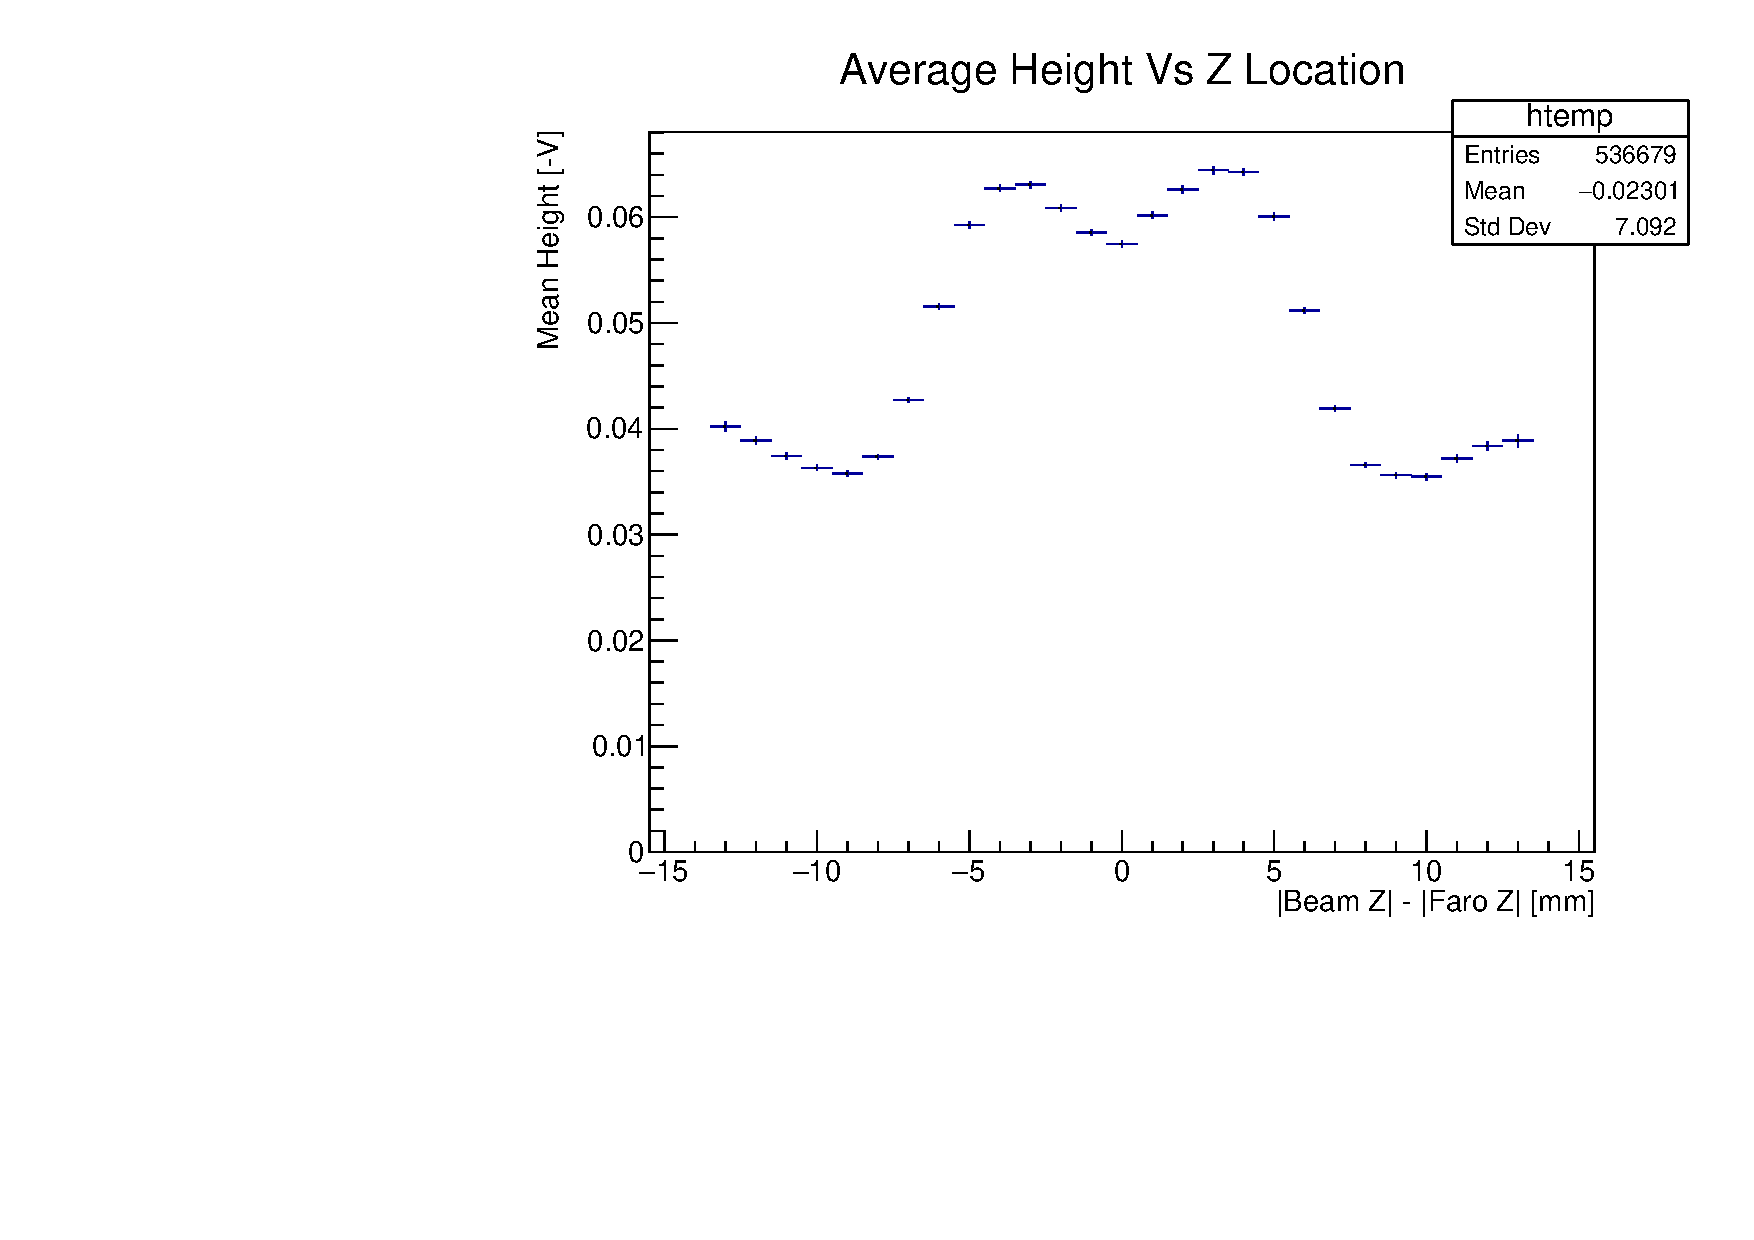
\includegraphics[width=4 cm]{graphics/heightvsz.pdf}
\caption{Average charge (left), height (right) in an event relative to measurement location on MPPC}
\label{fig:heightvzplot}
\end{figure}

\begin{figure}
\centering
    
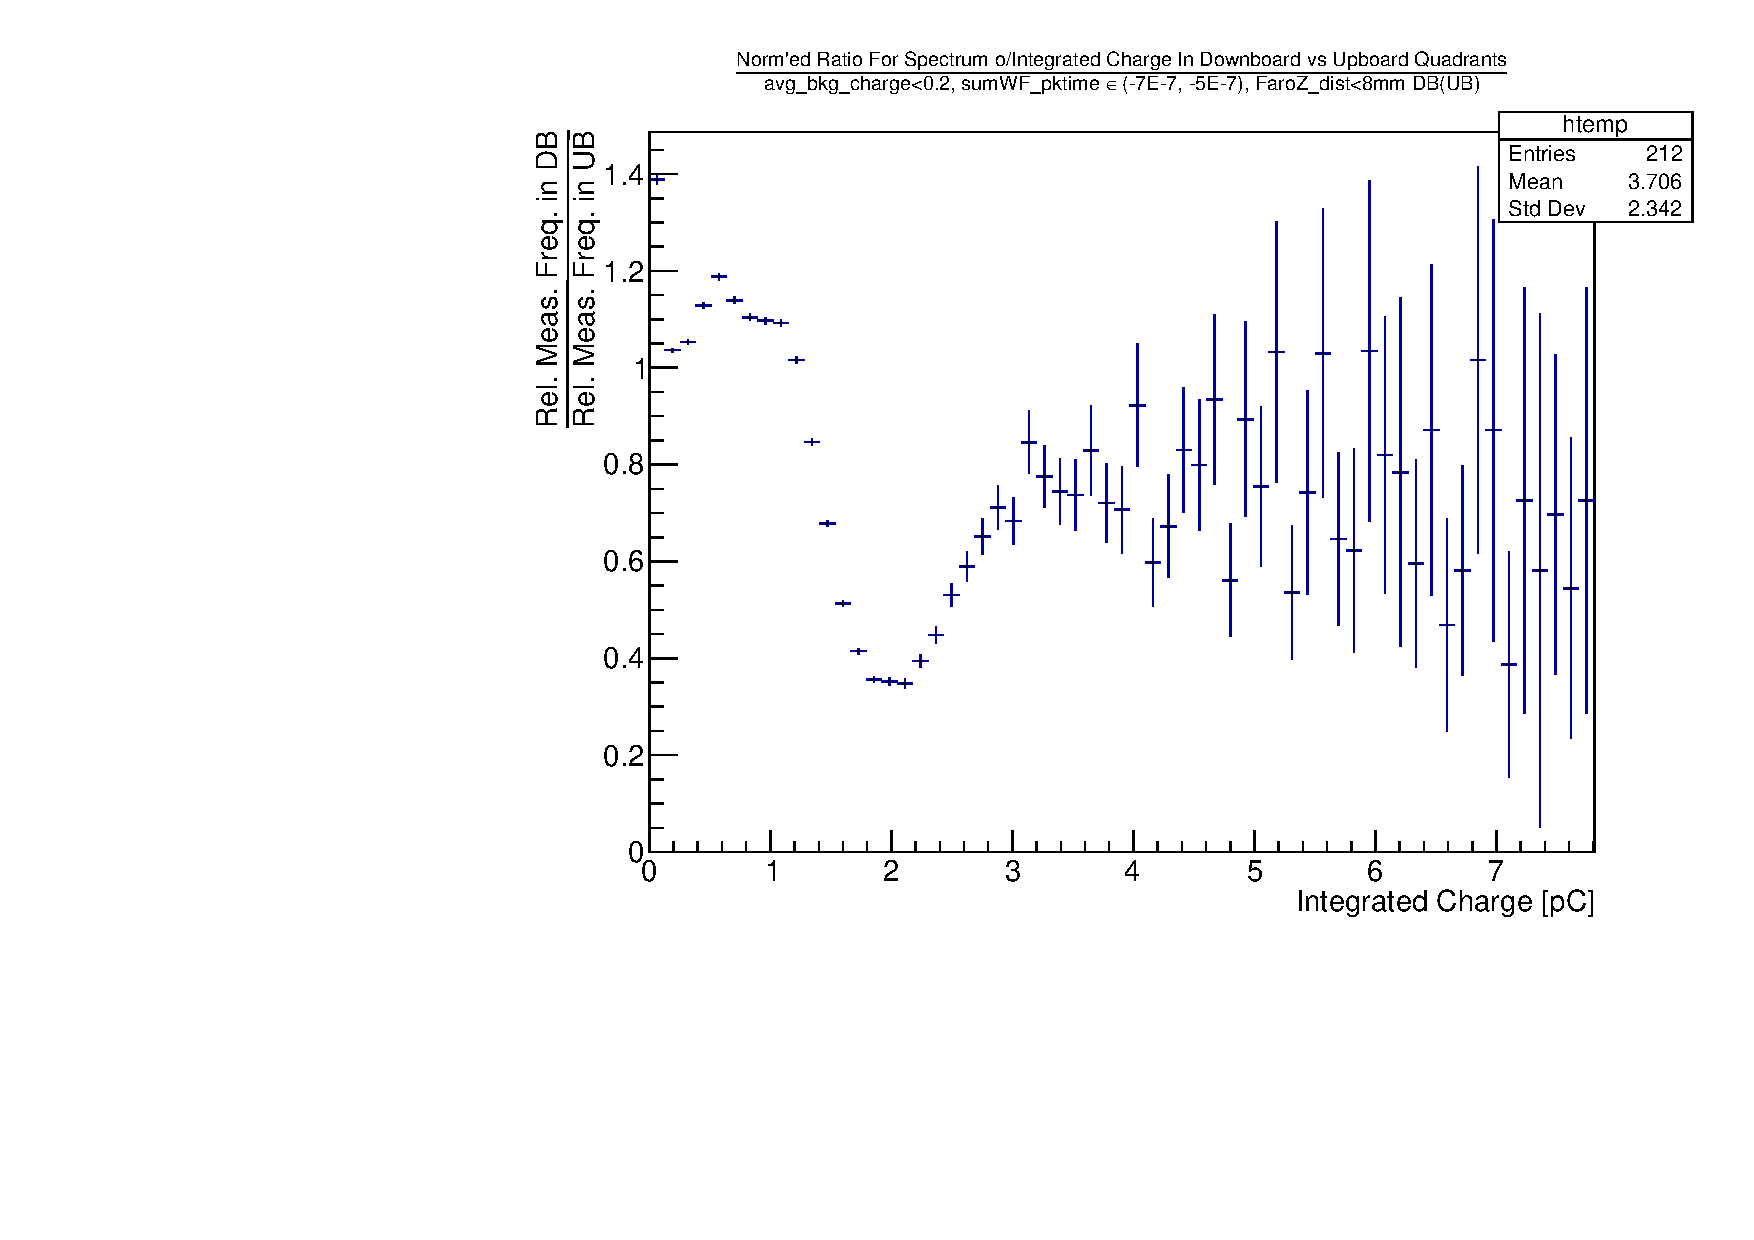
\includegraphics[width=4 cm]{graphics/chargeratiospectrum_DBtoUB.pdf}
\includegraphics[width=4 cm]{graphics/heightratiospectrum_DBtoUB.pdf}
\caption{Ratio of normalized charge (left), height (right) distributions in each MPPC half}
\label{fig:heightspectrumplot}
\end{figure}

\begin{table}[H]
    \centering
    \begin{tabular}{c||c|c|c}
         & DB Peak & UB Peak & Ratio \\
         \hline
        Charge & 0.777548 pC & 0.860434 pC & 0.903669 \\
        Height & 63.336 mV & 65.0873 mV & 0.973094
    \end{tabular}
    \caption{Amplitude of Height and Charge Distributions For MPPC Halves }
    \label{tab:qandhhalves}
\end{table}




Additionally, we are interested in the relative response between the two MPPC halves across the range of charge and height measurements.
Figure \ref{fig:heightspectrumplot} is especially interesting because these plots allow us to determine the differential nature in which the two sides will be effected by any alterations to the chosen threshold value. In the region of our selection criteria, the charge threshold will reject a higher number of events on the side closer to Z=0, whereas a selection on height effect both sides of the mppc equally. Moreover, this shift is in fact confirmed when we analyze the found mppc positions from both cuts, where a clear shift outwards from zero is present in the charge based cuts (Fig. \ref{fig:seldzvz}).
\begin{figure}
    \centering
    \includegraphics[width=5cm]{graphics/selectionshiftoverz.pdf}
    \caption{Difference in found positions under change from charge to amplitude selection}
    \label{fig:seldzvz}
\end{figure}








\section{Alternate Fit Function}
The set of well fit MPPCs were selected using the following critia,
\begin{enumerate}
    \item Uncertainty In Fit Mean $<$ 0.5 mm
    \item Uncertainty In Fit Sigma $<$ 0.5 mm
    \item Fit Width $\in$ (5.5mm,8.5mm)
    \item Reduced $\chi ^{2} \; <$ 4
\end{enumerate}

Comparing this set to the found positions from the piecewise fit function, we find the distribution contains very small offsets

\begin{figure}[h]
    \centering
    \includegraphics[width=.7\linewidth]{graphics/terdzhc.pdf}
    \includegraphics[width=.7\linewidth]{graphics/terdphc.pdf}
    \caption{Agreement In Found Z (top) and $\phi$ (bottom) Locations Between Fits}
    \label{fig:fitcompare}
\end{figure}


\appendix

\section{Fit Values and Errors}
Fitted parameter values and parameter errors for the primary fit 
function. 

\begin{enumerate}
    \item Z Position Fit Error $<$ 0.3 mm
    \item $\phi$ Position Fit Error $<$ 0.03 deg
    \item Reduced $\chi ^{2} \; <$ 100
\end{enumerate}


\begin{figure}[h]
    \centering
    \includegraphics[width=.4\linewidth]{plots/2018/ZMeanVal.pdf}
    \includegraphics[width=.4\linewidth]{plots/2018/ZMeanErr.pdf}\\
    \includegraphics[width=.4\linewidth]{plots/2018/ZSigmaVal.pdf}
    \includegraphics[width=.4\linewidth]{plots/2018/ZSigmaErr.pdf}\\
    \includegraphics[width=.4\linewidth]{plots/2018/ZWidthVal.pdf}
    \includegraphics[width=.4\linewidth]{plots/2018/ZWidthErr.pdf}\\
    \includegraphics[width=.4\linewidth]{plots/2018/ZSignalVal.pdf}
    \includegraphics[width=.4\linewidth]{plots/2018/ZSignalErr.pdf}\\
    \includegraphics[width=.4\linewidth]{plots/2018/ZNoiseVal.pdf}
    \includegraphics[width=.4\linewidth]{plots/2018/ZNoiseErr.pdf}
    \caption{Fitted parameter values (left) and errors (right) for Z position fits.}
    \label{fig:zfitpars}
\end{figure}

\begin{figure}[h]
    \centering
    \includegraphics[width=.4\linewidth]{plots/2018/PhiMeanVal.pdf}
    \includegraphics[width=.4\linewidth]{plots/2018/PhiMeanErr.pdf}\\
    \includegraphics[width=.4\linewidth]{plots/2018/PhiSigmaVal.pdf}
    \includegraphics[width=.4\linewidth]{plots/2018/PhiSigmaErr.pdf}\\
    \includegraphics[width=.4\linewidth]{plots/2018/PhiWidthVal.pdf}
    \includegraphics[width=.4\linewidth]{plots/2018/PhiWidthErr.pdf}\\
    \includegraphics[width=.4\linewidth]{plots/2018/PhiSignalVal.pdf}
    \includegraphics[width=.4\linewidth]{plots/2018/PhiSignalErr.pdf}\\
    \includegraphics[width=.4\linewidth]{plots/2018/PhiNoiseVal.pdf}
    \includegraphics[width=.4\linewidth]{plots/2018/PhiNoiseErr.pdf}
    \caption{Fitted parameter values (left) and errors (right) for $\phi$ position fits.}
    \label{fig:zfitpars}
\end{figure}


%\newpage
 


\section{Asymmetry Result Plots \bf [TEMPORARY]}

\subsection{Z Scans}

\begin{figure}[H]
\centering
\includegraphics[width=4cm]{asymmetryplots/azxwid2.pdf}
\includegraphics[width=4cm]{asymmetryplots/azxwid3.pdf}
\caption{Asymmetry width of two mppcs central in 4 wide trigger}
\label{fig:asymzwids} 
\end{figure}
\begin{figure}[H]
\centering
\includegraphics[width=4cm]{asymmetryplots/az-sgz2.pdf}
\includegraphics[width=4cm]{asymmetryplots/az-sgz3.pdf}
\caption{Asymmetry centers relative to supergaussian center fits}
\label{fig:asymzcentdiff} 
\end{figure}

\subsection{$\phi$ Scans}

\begin{figure}[H]
\centering
\includegraphics[width=4cm]{asymmetryplots/apxwid2.pdf}
\includegraphics[width=4cm]{asymmetryplots/apxwid3.pdf}
\caption{Asymmetry width of two mppcs central in 4 wide trigger}
\label{fig:asympwids} 
\end{figure}
\begin{figure}[H]
\centering
\includegraphics[width=4cm]{asymmetryplots/ap-sgp2.pdf}
\includegraphics[width=4cm]{asymmetryplots/ap-sgp3.pdf}
\caption{Asymmetry centers relative to supergaussian center fits}
\label{fig:asympcentdiff} 
\end{figure}

\end{document}
